\documentclass{article}
\usepackage{enumitem} 
\usepackage[T2A]{fontenc}
\usepackage[utf8]{inputenc}
\usepackage[ukrainian]{babel}
\usepackage[letterpaper,top=2cm,bottom=2cm,left=3cm,right=3cm,marginparwidth=1.75cm]{geometry}
\usepackage{amsmath}
\usepackage{graphicx}
\usepackage[colorlinks=true, allcolors=blue]{hyperref}
\usepackage{pgfgantt}
\usepackage{float}
\usepackage{hyperref}
\usepackage{listings}
\usepackage{xcolor}
\usepackage{booktabs}
\usepackage{makecell}
\usepackage{textcomp}

\lstset{
  language=Python,
  basicstyle=\ttfamily\small,
  keywordstyle=\color{blue},
  stringstyle=\color{red},
  commentstyle=\color{gray},
  showstringspaces=false,
  breaklines=true,
  frame=single
}


\title{Теоретичний матеріал для підготовки операторів засобів РЕБ та РЕР }
\author{\href{https://www.linkedin.com/in/eugene-usenko/}{Усенко Є.В.}, \href{https://www.linkedin.com/in/volodymyr-usenko-8409736b/}{Усенко В.В.}}

\begin{document}
\maketitle
\begin{abstract}
В процесі підготовки людей на операторів РЕБ та РЕР виявилося, що на поточний момент у слухачів курсу іноді не вистачає теоретичної бази. Цей короткий збірник призначений вирішити цю проблему і одночасно служити \textit{шпаргалкою} для тих, хто хоче оновити свої знання. Для зауважень та пропозицій можна використовувати систему зворотного зв'язку через створення \href{https://github.com/usnbros/sdr-dsp-book}{тікету на сторінці проєкту}.
\end{abstract}

\newpage
\tableofcontents

\newpage
\part{Теорія}
\section{Одиниці виміру}

Основні одиниці виміру, з якими нам доведеться стикатися в рамках цього курсу:

\begin{itemize}[noitemsep, topsep=8pt]
\item \textbf{Герци} — одиниця вимірювання частоти.
\item \textbf{Децибели} — одиниця виміру, яка показує відносну величину.
\item \textbf{Вати} — одиниця вимірювання потужності.
\end{itemize}

\subsection{Приставки Сі}
Оперуючи фізичними величинами, досить часто можна зустріти приставки: \textit{мілі-}, \textit{кіло-}, \textit{мега-}, \textit{гіга}-. Наприклад, \texttt{1мВт} (один міліват), \texttt{1МГц} (один мегагерц). У цьому блоці ми розглянемо приставки Сі, які будемо найбільше використовувати в подальшому навчальному матеріалі\footnote{Треба розуміти, що приставки Сі — це універсальний механізм, який працює для всіх фізичних величин, а не лише для тих, що перелічені в наступних секціях}.

Розглянемо приставки кратних одиниць, що перевищують основну фізичну величину на порядок, кратний 10. Тобто більше в 10, 100, 1000, тощо.

\begin{table}[ht]
\centering
\begin{tabular}{|l|l|l|}
\hline
\textbf{Множник} & \textbf{Приставка}  & \textbf{Приклад} \\
\hline
1000           & Кіло   & 1кГц дорівнює 1000Гц \\
1000 000       & Мега   & 1MГц дорівнює 1000кГц або 1000 000Гц \\
1000 000 000   & Гіга   & 1ГГц дорівнює 1000МГц \\
\hline
\end{tabular}
\caption{Приставки для множників частоти}
\end{table}

Найбільш розповсюджені випадки, з якими доведеться зіткнутися --- це перерахування частоти з МГц в ГГц і навпаки. Треба розуміти, що порядок між цими двома приставками кратний \texttt{1000}. \textbf{Щоб перевести МГц у ГГц, треба розділити значення частоти в МГц на 1000}. Наприклад, 850 МГц дорівнює 0.85 ГГц. \textbf{Щоб перевести ГГц у МГц, треба помножити значення частоти в ГГц на 1000}. Наприклад, 5.8 ГГц дорівнює 5800 МГц.

Для фізичних величин менше одиниці також є приставки.

\begin{table}[ht]
\centering
\begin{tabular}{|l|l|l|}
\hline
\textbf{Множник} & \textbf{Приставка}  & \textbf{Приклад} \\
\hline
0.001           & Мілі   & 1мВт дорівнює 0.0001Вт \\
0.000001        & Мікро  & 1мкВт дорівнює 0.000001Вт \\
\hline
\end{tabular}
\caption{Приставки для множників частоти}
\end{table}

\textbf{Щоб перевести мВт у Вт, треба поділити значення потужності в мВт на 1000}. Наприклад, 100 мВт дорівнює 0.1 Вт. \textbf{Щоб перевести Вт у мВт, треба навпаки помножити значення потужності у Вт на 1000}. Наприклад, 1.5 Вт дорівнює 1500 мВт.

\subsection{Частота}
Частота --- фізична величина, що дорівнює кількості однакових подій за одиницю часу. Вона є характеристикою будь-яких процесів, які регулярно повторюються (кількість подій за одиницю часу). Вимірюється в Герцах (Гц). Якщо сигнал виконує одне повне коливання (повний цикл) за секунду, то така частота дорівнює одному Герцу, якщо тисяча коливань за секунду --- 1 кіло Герц (кГц), якщо мільйон коливань --- 1 МГц, тощо.


\begin{figure}[h!]
\centering
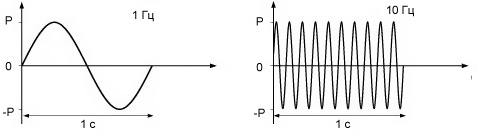
\includegraphics[width=0.7\linewidth]{images/frequency.png}
\caption{\label{fig:frequency}Гармонічний сигнал з частотою 1Гц(зліва) і 10Гц(справа).}
\end{figure}

\subsection{Потужність}
Визначення потужності як фізичної величини звучить наступним чином --- це робота, виконана за одиницю часу, або енергія, передана за одиницю часу. Вимірюється у Ватах (Вт). Також, коли ми будемо оперувати відносними величинами потужності, то часто зустрічатимемо потужність, позначену у dBm (децибел-міліват, див. наступну секцію \ref{sec:db}).


\subsection{Відносні величини}
\label{sec:db}
Коли потрібно порівнювати які-небудь величини, це можна зробити по-різному. Наприклад, можна розділити одне значення на інше і отримати порядок, який вказує, у скільки разів відрізняються значення. А якщо ми оперуємо абсолютними величинами, наприклад, \texttt{0.0000000001 - 100000000}, то відношення між двома такими величинами буде ще більшим, ніж фактичні значення.

Основна причина, чому використовуються децибели, полягає в тому, що фізична величина може змінюватися в дуже широкому діапазоні. Наприклад, співвідношення сигнал/шум (т.з. signal noise ratio або скорочено SNR) може бути настільки великим у абсолютному вираженні, що нам довелося б оперувати числами з багатьма нулями, що дуже незручно. Тому для таких величин і випадків використовують логарифмічну шкалу -- децибели. Важливо пам'ятати:
\begin{itemize}[noitemsep, topsep=8pt]
\item Децибели --- це відносне значення, яке показує порядок підсилення або затухання.
\item Шкала в децибелах нелінійна, тобто \texttt{10Дб} і \texttt{100Дб} фактична величина буде відрізнятися не в \texttt{10} разів, а в \texttt{1000 000 000}.
\item Негативне значення в \texttt{Дб} означає, що фактична величина не негативна, а лише менша за одиницю.
\end{itemize}


\subsection{dBm}
Також потрібно розуміти, що коли ми говоримо про децибели, то зазвичай це робимо у прив'язці до якоїсь фізичної величини. Наприклад, рівень потужності в децибелах відносно \texttt{1мВт} називається \textbf{dBm} (децибел-міліват).


\begin{table}[h!]
\centering
\begin{tabular}{|c|l||c|l|}
\hline
\textbf{dBm}  & \textbf{мВт} & \textbf{dBm} & \textbf{мВт} \\
\hline
100  & 10000000000  &  -1  & 0.794 \\
90   & 1000000000   &  -3  & 0.501  \\
80   & 100000000    &  -6  & 0.251  \\
70   & 10000000     & -10  & 0.1 \\
60   & 1000000      & -20  & 0.01 \\
50   & 100000       & -30  & 0.001 \\
40   & 10000        & -40  & 0.0001 \\
30   & 1000         & -50  & 0.00001 \\
20   & 100          & -60  & 0.000001 \\
10   & 10           & -70  & 0.0000001 \\
 6   & 3.981        & -80  & 0.00000001 \\
 3   & 1.995.       & -90  & 0.000000001 \\
 1   & 1.259        & -100 & 0.0000000001 \\
\hline
\end{tabular}
\caption{\label{table:dbm2mwatts}Співвідношення dBm до мВт}
\end{table}

Декілька прикладів:
\begin{itemize}[noitemsep, topsep=8pt]
\item Потужність WiFi роутера в середньому складає \texttt{17dBm} (приблизно \texttt{0.05Вт}).
\item Потужність мобільного телефона приблизно складає \texttt{33dBm} (приблизно \texttt{2Вт}).
\item Потужність антидронової рушниці складає \texttt{40dBm} (дорівнює \texttt{10Вт}).
\end{itemize}

На практиці співвідношення значень \texttt{dBm до мВт} зазвичай мало хто знає або пам'ятає на пам'ять --- це нормально. Для конвертації можна використовувати наведену Табл. \ref{table:dbm2mwatts} або онлайн калькулятори: \href{https://www.everythingrf.com/rf-calculators/dbm-to-watts}{dBm в Вт} та \href{https://www.everythingrf.com/rf-calculators/watt-to-dbm}{Вт в dBm}.
\subsection{dBi}


\textbf{dBi} (decibels isotropic) --- це одиниця вимірювання підсилення антен відносно \textit{еталонної} антени. За таку еталонну антена прийнято т.зв. ізотропний випромінювач — ідеальна антена, діаграма спрямованості якої є сферою, коефіцієнт підсилення дорівнює одиниці, а ККД — 100\%. Випромінювання сигналу такою антеною відбувається з рівномірною інтенсивністю в усі сторони. Такої антени в природі не існує, це віртуальний об'єкт, однак дуже зручний як еталон для вимірювання параметрів реальних антен.

Існує ще одна одиниця: dBd -- тут за еталон прийнято напівхвильовий диполь. Проте використання dBi є більш зручним, оскільки в цьому випадку легше проводити розрахунок енергетичного балансу. dBi -- це відносна одиниця, яка по суті нічим не відрізняється від звичайного децибела, за винятком визначення еталону, відносно якого ведеться відлік.

Принципової різниці між dBi і dBd немає -- підсилення в dBi = підсиленню в dBd + 2,15 dB. У старих радіоаматорських книжках і журналах підсилення антен вимірюють просто в децибелах. У такому випадку, найчастіше мається на увазі підсилення відносно напівхвильового вібратора, тобто воно еквівалентне dBd. Вимірювання відносно ізотропного випромінювача спочатку використовувалося тільки в США, але останнім часом поширилося по всьому світу, тому для уникнення плутанини зараз, якщо йдеться про підсилення антени, правилом гарного тону вважається використання децибела з суфіксом -- dBi або dBd.


\begin{itemize}[noitemsep, topsep=8pt]
\item \textbf{Ізотропний випромінювач} -- це ідеальна модель антени, яка випромінює однаково у всіх напрямках. Хоча такі антени не існують на практиці, їх використовують як базу для порівняння.
\item \textbf{Коефіцієнт підсилення} в dBi показує, наскільки антена спрямована. Наприклад, якщо антена має підсилення 6 dBi, це означає, що в певному напрямку вона випромінює в 4 рази більше енергії $(10^{\frac{6}{10}} \approx 4)$, ніж ізотропний випромінювач.
\item \textbf{Чим вищий показник} dBi, тим більш спрямованою є антена, що означає, що вона концентрує більше енергії в одному напрямку, але менше випромінює в інші.
\end{itemize}

\textbf{Приклад.} Антена з підсиленням 3 dBi випромінює приблизно вдвічі більше енергії в певному напрямку порівняно з ізотропним випромінювачем. Якщо підсилення антени становить 9 dBi, це означає, що антена має значно кращу спрямованість і концентрує енергію ще вужче в одному напрямку.

\section{Радіохвилі}

\textbf{Радіохвилі} -- це тип електромагнітного випромінювання з довжиною хвиль понад 1 мм (частотою нижче 300 ГГц). Неформально визначення радіохвиль можна пояснити як електромагнітну енергію у просторі. Це є основою для розуміння певних явищ радіохвиль, звісно, як аналогія.

\begin{figure}[h!]
\centering
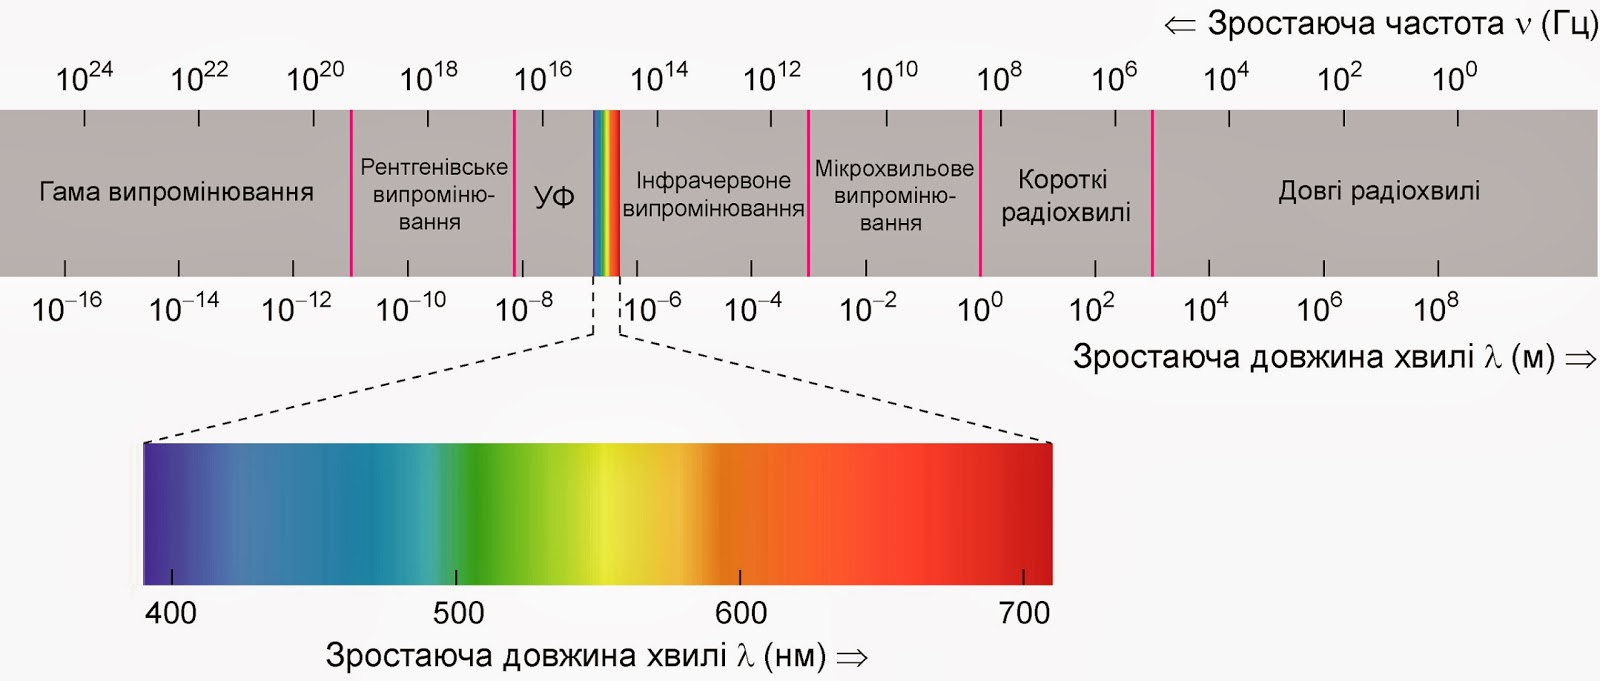
\includegraphics[width=0.9\linewidth]{images/electromagnetic-range.jpg}
\caption{\label{fig:electromagnetic}Діапазон радіохвиль на загальному спектрі електромагнітних хвиль.}
\end{figure}

Довжина хвилі може бути обчислена за адаптованою формулою:

\[
\lambda = \frac{300}{f}
\]

\begin{itemize}[noitemsep, topsep=8pt]
\item $\lambda$ -- довжина хвилі в метрах
\item ${f}$ -- частота хвилі в \texttt{МГц}
\end{itemize}

Коли ми говоримо про радіохвилі, то зазвичай оперуємо частотою в Гц з різними приставками (МГц, ГГц, тощо) -- але інколи можемо зустріти розмірність в метрах, міліметрах та сантиметрах. Якщо знаємо довжину хвилі і треба порахувати частоту, то виконуємо наступну послідовність -- переводимо довжину хвилі у метри, \texttt{300} ділимо на це значення (отримаємо частоту в МГц).

Розуміння довжини хвилі потрібно в контексті розміру антен. На практиці зустрічаються антени, розміри яких дорівнюють \texttt{$\lambda$/2} або \texttt{$\lambda$/4}.

\textbf{Приклад 1}. Для спектроаналізатора типу TinySA доволі часто використовується направлена логоперіодична антена на діапазон частот \texttt{600МГц - 6ГГц}. В цьому типі антен ширина кожного вібратора дорівнює \texttt{$\lambda$/2}. За формулою найширша частина антени буде \texttt{300/600МГц}, що дорівнює \texttt{0.5м} і відповідає повній довжині хвилі, а половина цього значення (\texttt{$\lambda$/2}) -- це \texttt{25см}.

\textbf{Приклад 2}. Ми знайшли ворожий дрон з антеною горизонтальної поляризації \href{https://modelistam.com.ua/images/dl-ant-rx60.jpg}{типу діполь}. Довжина антени складає \texttt{17.6см}. Питання: на яку частоту нам потрібен РЕБ? Спочатку переведемо сантиметри в метри, що дорівнює \texttt{0.176м}. Далі, знаючи, що для цього типу антен довжина складає половину довжини хвилі, то відповідна повна довжина буде \texttt{2*0.176 = 0.352м}. Щоб отримати робочу частоту керування дрона, застосовуємо формулу \texttt{300/0.352 = 852МГц}. Тобто, нам потрібен РЕБ на діапазон \texttt{800 - 900МГц}.

\subsection{Радіочастотні діапазони}

\textbf{Радіочастотні діапазони} - це певні інтервали радіочастот, які використовуються для різних видів радіозв'язку та передачі даних. Кожен діапазон має свої унікальні характеристики, такі як дальність поширення, здатність проникати крізь перешкоди та пропускна здатність, що визначає їх застосування.

\begin{table}[ht]
	\centering
	\begin{tabular}{|l|l|l|}
		\hline 
		\textbf{Найменування}  & \textbf{Повна назва} & \textbf{Діапазони} \\
		\hline
		VLF      	& Very low frequencies		& 3 - 30 kHz   		\\
		LF    		& Low frequencies    		& 30 - 300 kHz 		\\
		MF			& Medium frequencies		& 300 - 3000 kHz	\\
		HF    		& High frequencies			& 3 - 30 MHz 		\\
		VHF     	& Very high frequencies 	& 30 - 300 MHz  	\\
		UHF			& Ultra high frequencies	& 300 - 3000 MHz	\\
		SHF			& Super high frequencies	& 3000 - 30000 MHz 	\\
		\hline
	\end{tabular}
	\caption{\label{table:radiowaves_types} Таблиця класифікації радіохвилі по діапазонам}
\end{table}

Із цієї номенклатури класифікацій нас більше усього цікавлять хвилі в діапазонах VHF, UHF та частково SHF до 6-8 GHz.


\subsection{Розповсюдження радіохвиль}

\textbf{Розповсюдження радіохвиль} — це процес, під час якого радіохвилі передаються від передавача до приймача через різні середовища: повітря, вода, іонізовані шари атмосфери тощо. Природа розповсюдження радіохвиль має певні особливості, що напряму залежать від фізичних властивостей самої хвилі, частоти та її довжини. Фізичні властивості хвилі визначають їх межі та області застосування.

\begin{figure}[h!]
	\centering
	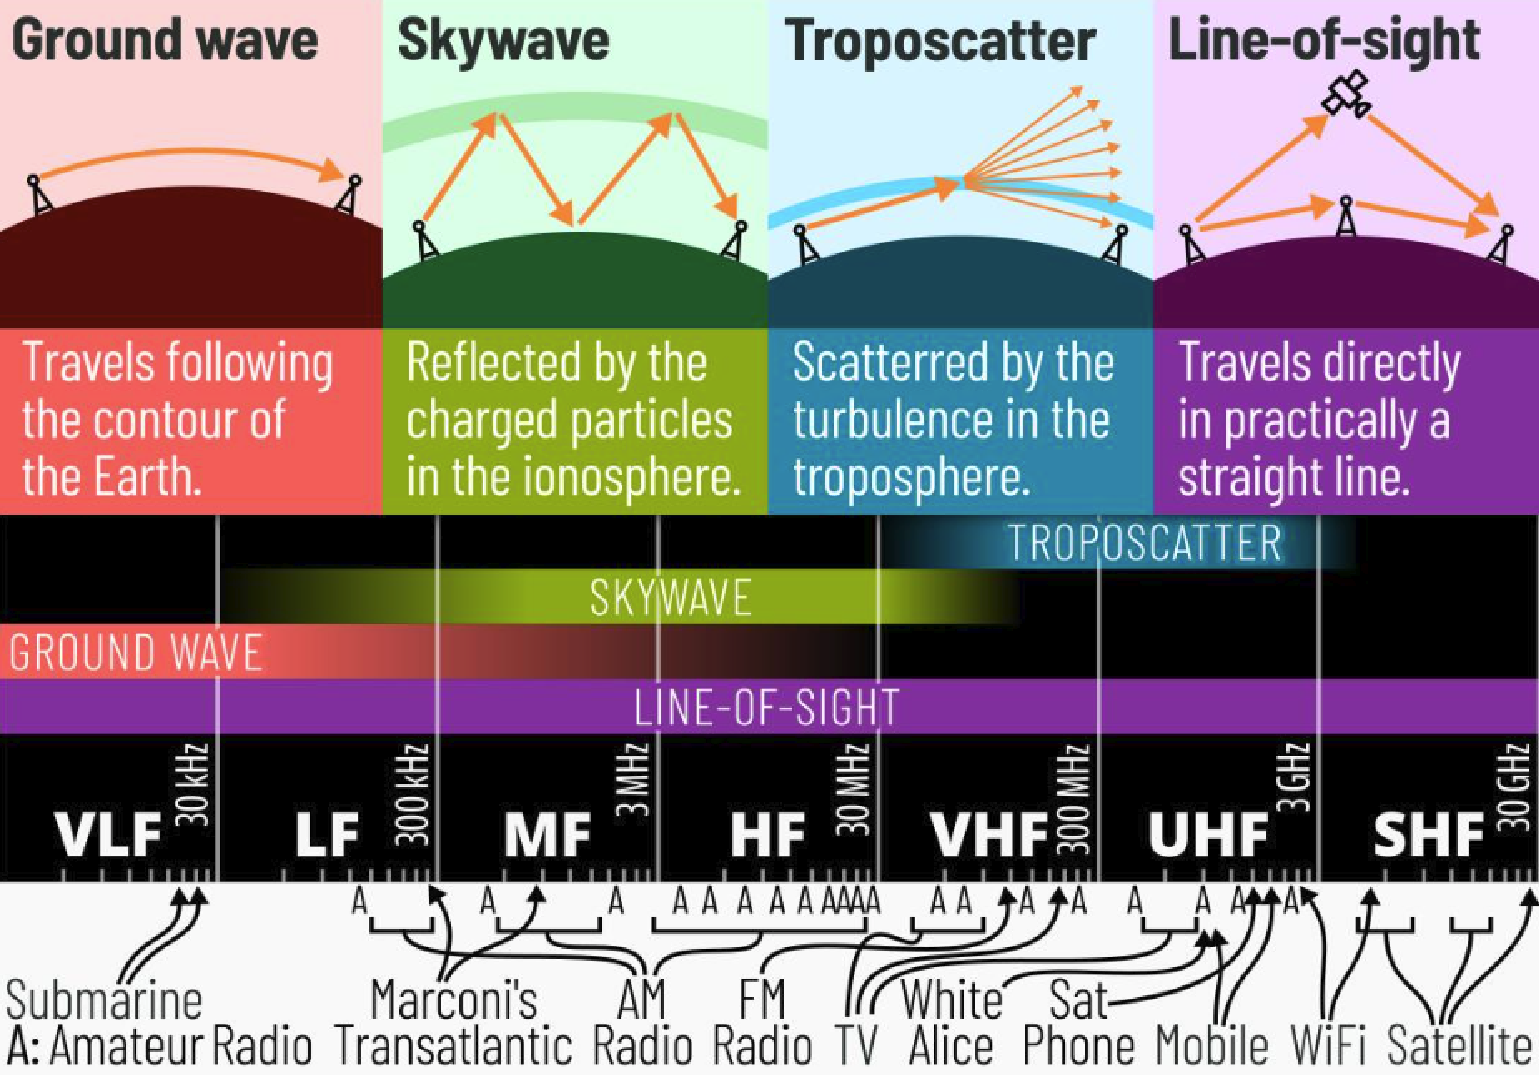
\includegraphics[width=0.8\linewidth]{images/radio-propagation.png}
	\caption{\label{fig:radio-propagation} Розповсюдження радіохвиль}
\end{figure}


\begin{itemize}[noitemsep, topsep=8pt]
	\item VLF - дуже стійка наземна хвиля, проходить крізь воду.  Застосовується серед військових для підводного зв'язку. Майже не відбивається і не затухає на великих відстанях.
	\item LF - розповсюдження наземне, особливо ефективне над морем.
	Використовуються в навігація (LORAN), маяках та морському зв'язку. 
	\item MF - розповсюдження вдень відбувається зазвичай наземне, вночі за рахунок відбуття від іоносфери. Середня дальність застосування, має помітне затухання вдень. AM-радіо, морська/авіаційна навігація (NDB), надводний зв'язок.
	\item HF - розповсюдження за рахунок відбиття від іоносфери, використовується для дальнього радіозв’язку серед військових, а також в авіації.
	\item VHF - розповсюдження відбувається за рахунок прямої видимості або за рахунок заломлення у тропосфері. Застосовуються зазвичай у FM-радіо, телебаченні, 
	наземних та портативних радіостанціях (раціях) або для керування дронами. 
	\item UHF - розповсюдження виключано за рахунок прямої видимості, легко поглинається матеріалами (стінами, лісом і т.д.). Мають особливість зумовлену малим радіусом дії без ретрансляції, але зручно для використання в міських умовах.
	\item SHF - розповсюдження виключно в межах прямої видимості, велика чутливість до зовнішнього середовища, а саме температури, тиску, вологості повітря і т.д. Має дуже слабке проникнення, вимагає застосування спрямованих антен.
\end{itemize}

Як ми вже зрозуміли, що природа поширення радіохвиль для різних частот буде різна, але для всих цих діапазонів працює одне основне правило, що їх поєднує, а саме те, що незалежно від діапазону передача інформація може відбуватись в зоні прямої видимості. Тому ми наближаємось до поняття радіогоризонту.   

\textbf{Радіогоризонт} -- це максимальна відстань від антени до точки на земній поверхні, де радіохвилі ще можуть бути прийняті при прямій видимості. Іншими словами, це межа, за яку радіосигнал перестає поширюватися по прямій лінії через кривизну Землі. Радіогоризонт збільшується з висотою антени або розташування її на максимальній висоті. Чим вище антена, тим далі поширюється сигнал.

\begin{figure}[h!]
\centering
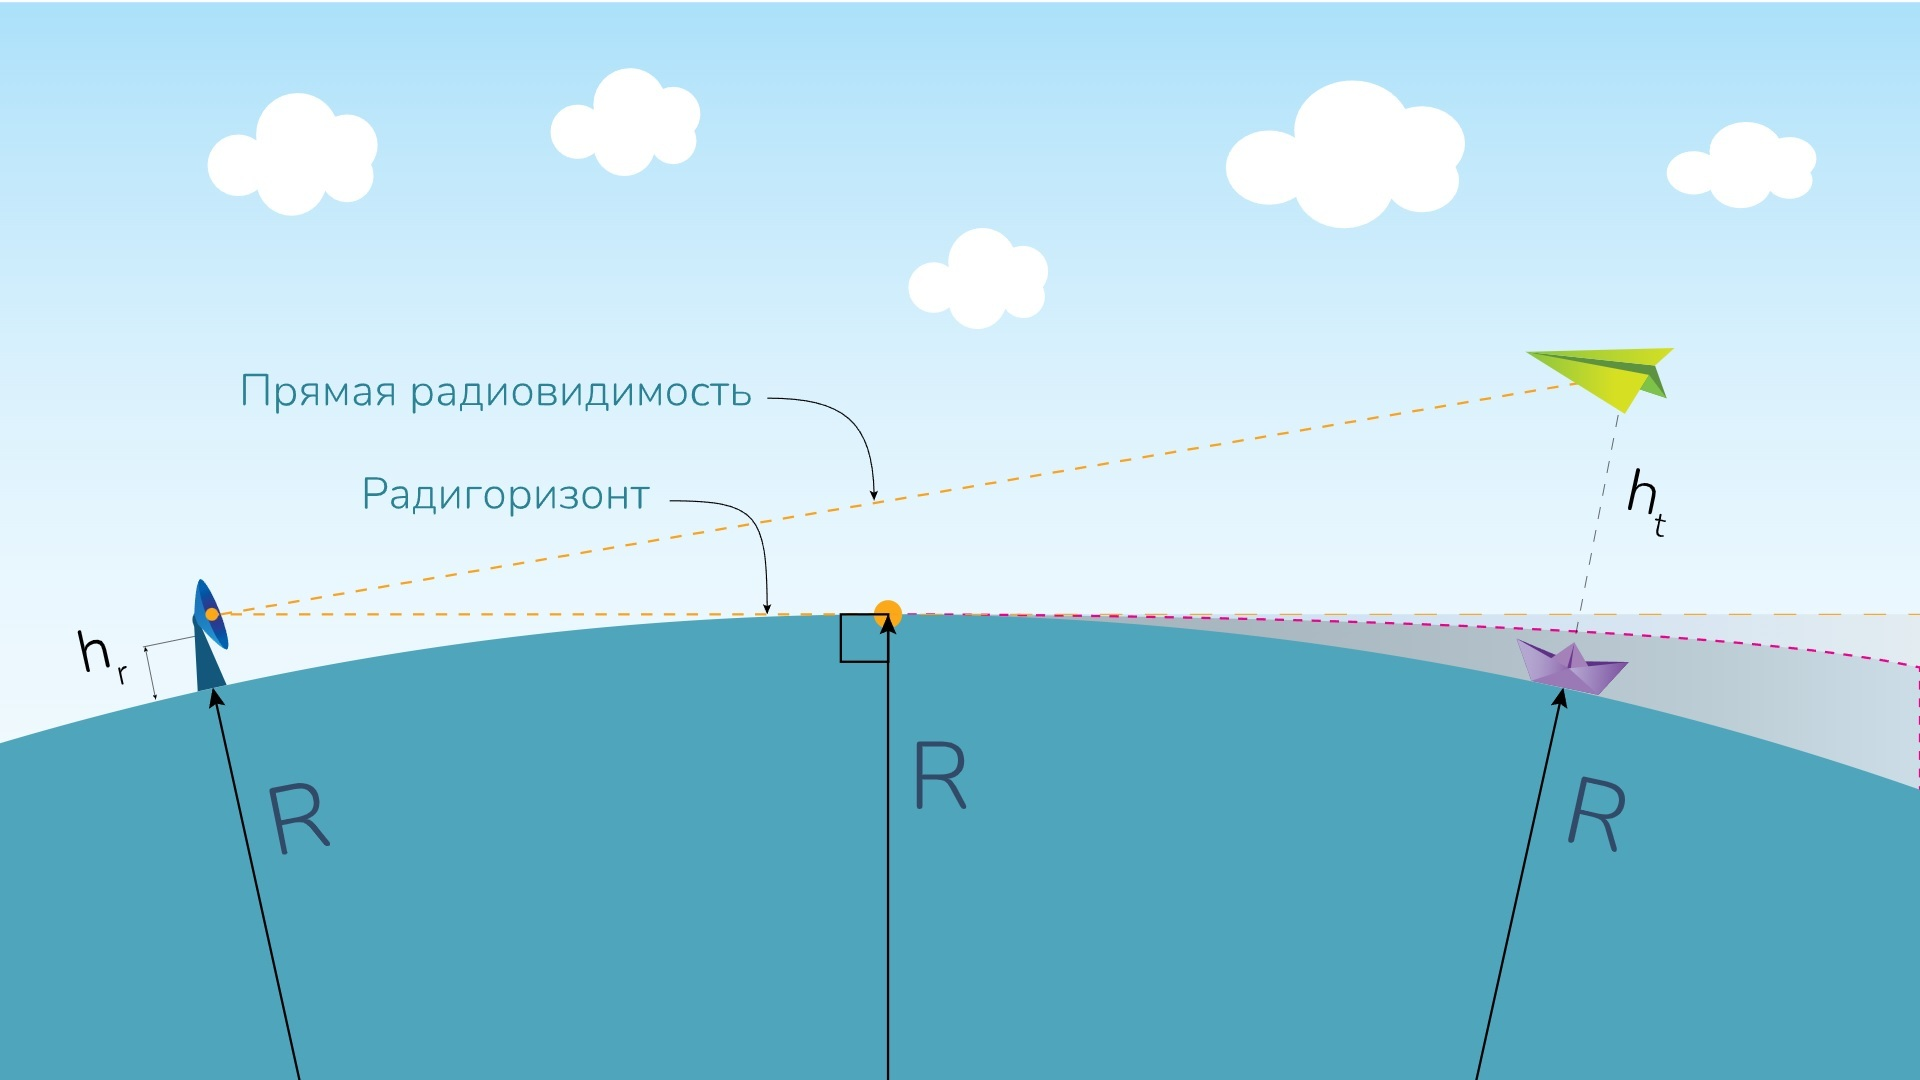
\includegraphics[width=0.6\linewidth]{images/radio-horizon.jpeg}
\caption{\label{fig:radio-horizon}Радіогоризонт}
\end{figure}

\subsection{Рефлексія радіохвиль}

\textbf{Рефлексія радіохвиль} --- це відбиття радіохвиль від перешкод, яке призводить до зміни напрямку розповсюдження радіохвилі. В залежності від задачі це може мати, як і позитивні, так і негативні наслідки. В контексті виявлення джерел радіовипромінювання пеленгаційними системами, це ускладнює процес визначення оригінального напрямку джерела раідовипромінювача, осболиво, якщо вібиття відбувається хаотично в різні напрямки, що приводить до ситуації, коли одне і те самє радіоджерело надходить з різних напрямків. Такє відбиття називається дифузним, але відбиття також може бути і дзеркальним. 

\begin{figure}[h!]
	\centering
	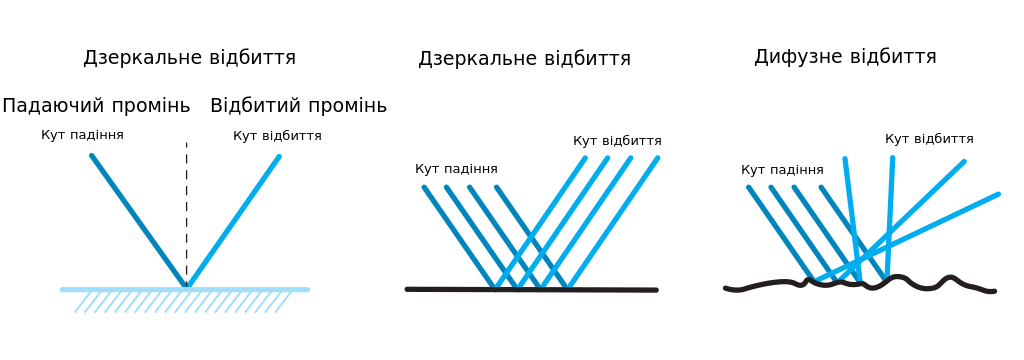
\includegraphics[width=0.8\linewidth]{images/reflection.png}
	\caption{\label{fig:reflection}Рефлексія радіохвиль}
\end{figure}

Дзеркальне відбиття має доволі просту природу і визначається тим, що кут падіння проміню буде відповідати куту його відиття, тобто кути будуть дзеркально-симетричними. Наприклад, якщо ви працюєте за пеленгатором і знаєте, що джерело радіовипромінювання знаходиться за певним напрямком, але пеленгаційна система визначає його, як протилежний у 180 градусів від очікуваного, то ви точно зіткнулись із перевідбиттям. Радіохвилі можуть відбиватися від різних поверхонь, таких як земля, будівлі, металеві предмети, водойоми та предмети, що утримують в собі вологу.

\newpage
\subsection{Рефракція радіохвиль}

\textbf{Рефракція радіохвиль} --- це зміна траєкторії радіохвилі під впливом середовища. Температура, тиск і вологість впливають на швидкість поширення радіохвиль у просторі, як результат на зміну напрямку для VHF та UHF діапазонів. Швидкість поширення хвиль в різних середовищах різна, як б це дивно не звучало, довжина хвилі в цьому випадку теж міняється, але тут варто зазначити, що це ніяким чином не впливає на її частоту.  

\begin{figure}[h!]
	\centering
	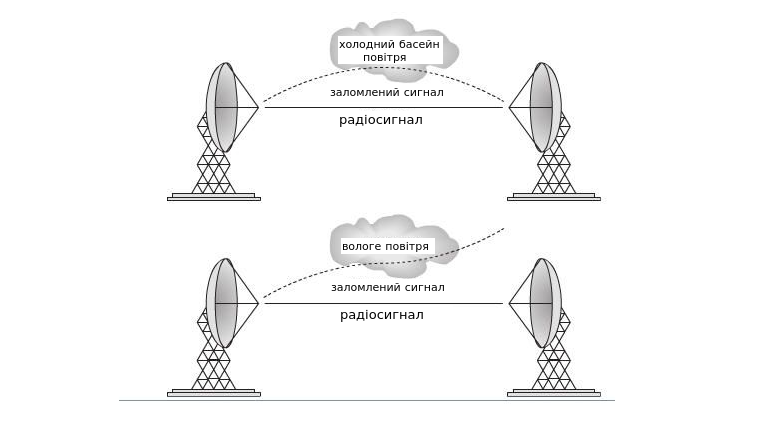
\includegraphics[width=0.8\linewidth]{images/refraction.png}
	\caption{\label{fig:refraction}Рефракція радіохвиль}
\end{figure}


Завдяки такій фізичній властивості, ми можемо відправляти інформацію на дуже далекі відстані за раідогоризонт, оминати перешкоди за рахунок заломлення радіохвиль від іоносфери для HF діапазону.

\begin{figure}[h!]
	\centering
	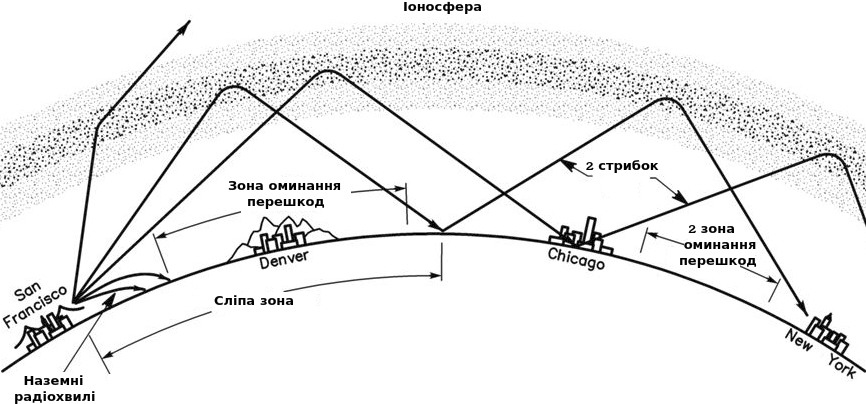
\includegraphics[width=0.8\linewidth]{images/refraction2.png}
	\caption{\label{fig:refraction2}Рефракція в іоносфері}
\end{figure}



\subsection{Дифракція радіохвиль}

\textbf{Дифракція радіохвиль} --- це здатність радіохвиль оминати перешкоди на своєму шляху, що дозволяє досягати сліпих зон, але при цьому істотно втрачати потужність. Тут варто зазначити, що дифракці має пряму залежність від довжини хвилі, чим більше довжина хвилі і меньше частота, тим краще вона долає перешкоди, тобто хвилі в діапазонах HF, VHF краще огинають перешкоди ніж в діапазонах UHF. Сам ефект, зазвичай, може проявлятись в момент при зіткненні хвилі об края перешкод або при проходженні хвилі через щілини. Радіохвилі також здатні буквально огинати перешкоди на своєму шляху, але за умови, якщо перешкода є меньшою за довжину хвилі.

\begin{figure}[h!]
	\centering
	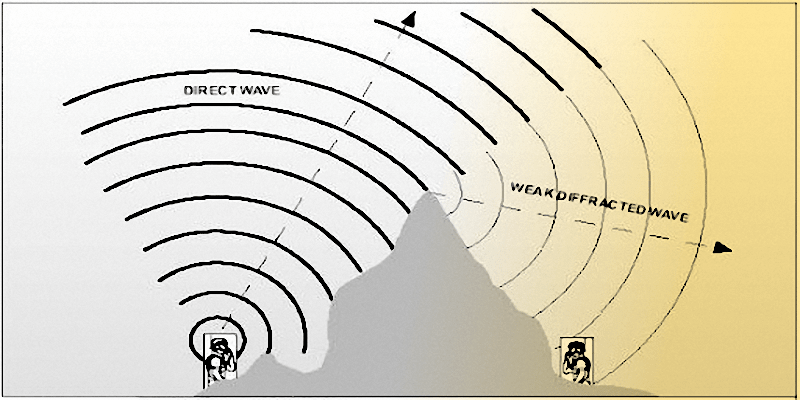
\includegraphics[width=0.8\linewidth]{images/diffraction.png}
	\caption{\label{fig:diffraction}Дифракція та перешкоди}
\end{figure}

Окрім позитивних ефектів, він також має і негативний для пеленгаційних систем, бо є хибним азимутом джерела випромінювання. Огинаючи перешкоди радіохвиля міняє свій істиний азумут і як у випадку з рефракцією та рефлексією створює хибний кут джерела випромінювання. 
\begin{figure}[h!]
	\centering
	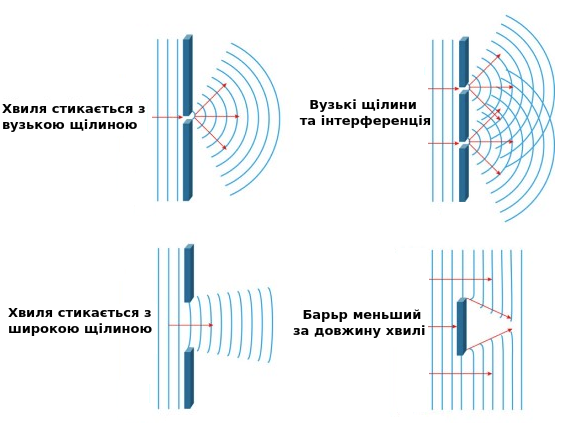
\includegraphics[width=0.6\linewidth]{images/diffraction_all.png}
	\caption{\label{fig:diffraction_all} Дифракція радіохвиль}
\end{figure}

\subsection{Інтерференція радіохвиль}

\textbf{Інтерференція радіохвиль} --- це явище, яке взаємно збільшується або зменшується в результаті підсумовування амплітуд хвиль, що поширюються в просторі. Результат інтерференції залежить від різниці фаз: в одному випадку амплітуда збільшується (співпадіння по фазі, мал. \ref{fig:interferense} зліва), а в іншому зменшується (хвилі в протифазі, мал. \ref{fig:interferense} справа).

\begin{figure}[h!]
\centering
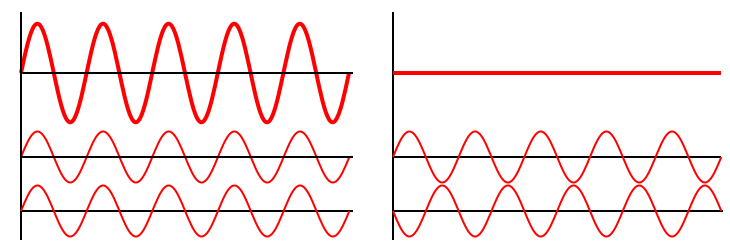
\includegraphics[width=0.7\linewidth]{images/interferense.png}
\caption{\label{fig:interferense}Інтерференція радіохвиль}
\end{figure}

Наприклад, в контексті РЕБ-у,якщо антени модуля РЕБ будуть близько розташовані і які будуть працювати на одному або суміжних діапазоні, можуть значно зменшувати ефективність подавлення через вплив одна на одну, коли радіохвилі випромінюються у протифазі. Як наочний приклад такої взаємодії хвиль можна спостерігати у природі, наприклад, на поверхні води, коли хвилі від різних джерел впливають одна на одну (мал. \ref{fig:two-emmitions}).

\begin{figure}[h!]
\centering
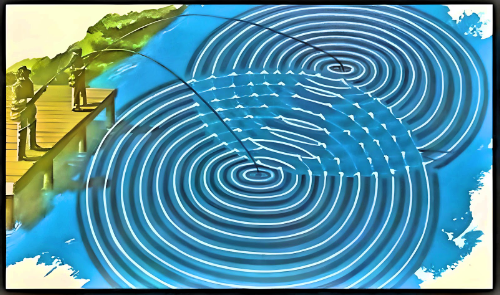
\includegraphics[width=0.6\linewidth]{images/two-emmitions.png}
\caption{\label{fig:two-emmitions}Взаємний вплив різних джерел хвиль.}
\end{figure}

\subsection{Федінг радіохвиль}

\textbf{Федінг радіохвиль} --- це саме звичайне затухання радіохвиль у просторі. Затухання радіохвиль залежить від частоти. Чим вища частота, тим сильніше затухання, але залежність не є лінійною і залежить від багатьох факторів. Із самого елементарного можуть впливати погода та атмосферний тиск. Але тут ми поговоримо про більш складний комплексний процес, що має більш сумарний ефект усих явищ, які ми розглядали перед цим. Справа у тому, що сигнал надходить до приймача кількома шляхами, а саме із-за перевідбитів, дифракцій та розсіювань ці шляхи мають різну довжину, тому сигнали надходять в різних фазах. Коли ці сигнали попадають у фазу, то сигнал посилюється. Коли вони деструктивно інтерферують, тобто попадають у протифазу, вони компенсують один одного, спричиняючи згасання, що і є федінгом в т.ч.

\textbf{Приклад}: Уявіть, що ви йдете містом зі своїм телефоном. Ви знаходитесь у місці, де на ваш телефон потрапляє як прямий, так і відбитий сигнал. Коли ви рухаєтесь на кілька сантиметрів, сигнали можуть переходити від конструктивних до деструктивних перешкод і приходити у протифазі на ваш телефон. Рівень сигналу, що відображається на вашому телефоні, коливається — це і той самий федінг. Тут ми підходимо до поняття інтерференції радіохвиль.

\subsection{Зона Френеля}

\textbf{Зона Френеля} --- це еліптична область, що оточує лінію прямої видимості, яка з'єднує дві точки бездротової мережі. Між цими двома точками електромагнітна хвиля набуває форми еліпсоїда, він формується навколо лінії видимості (Line-of-Sight). Для гарної якості сигналу різні перешкоди місцевості (елементи рельєфу, будівлі, дерева) не повинні перетинати не тільки лінію прямої видимості, а і зону Френеля.  Максимальний радіус еліпсоїда у центральній частині, залежить від двох параметрів - частоти та відстані. Знаючи частоту та відстань між точками, можна розрахувати максимальний радіус зони Френеля у центральній точці між двома антенами.

\begin{figure}[h!]
	\centering
	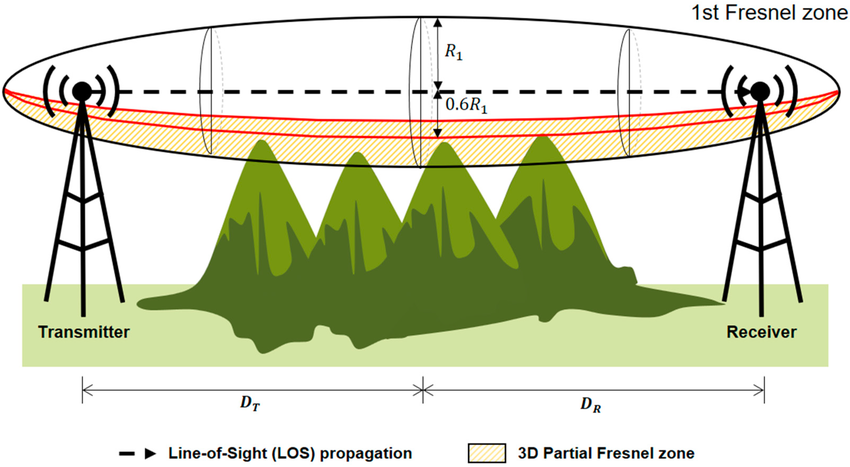
\includegraphics[width=0.9\linewidth]{images/fresnel-zone.png}
	\caption{\label{fig:fresnel-zone} Зона Френеля.}
\end{figure}

Зону Френеля потрібно знати і вміти розраховувати, бо це дає розуміння, як будувати зв'язок за рахунок WIFI мостів, або інших меш мереж, комунікацій між наземною станцію та БПЛА, а також для ефективного застосування РЕБ-у. Для себе можно визначаити оптимальне правило, що 60 відсотків першої зони Френеля повинно бути вільним від перешкод, якщо ми хочемо мати більш-менш стабільну передачу інформації. Розрахувати зону Френеля в метрах можно за наступною формулою:


\[
R_1 = 17.32 \cdot \sqrt{\frac{d_t \cdot d_r}{f \cdot (d_t + d_r)}}
\]

\begin{itemize}[noitemsep, topsep=8pt]
	\item $R1$ -- перша зона Френеля
	\item $dt,dr$ -- відстані до точки центру зони від передавача та приймача (у \texttt{км})
	\item ${f}$ -- частота в \texttt{GHz}
\end{itemize}

\textbf{Приклад}: Відстань між точками складає 1 км, частота - 2.4 GHz і робимо наступні розрахунки за формулою.

\[
R_1 = 17.32 \cdot \sqrt{\frac{0.5 \cdot 0.5}{2.4 \cdot (0.5 + 0.5)}}=17.32 \cdot \sqrt {\frac{0.25}{2.4}}=5.59 м
\]

Відстань між двома антенами складає 1 км, відповідно відстань до центру буде складати по 0.5 км. Застосувавши формулу, ми визначили радіус першої зони Френеля і він складає 5.59 метри. Попередньо було зазначено, що мінімальна необхідна зона без перешкод має складати мінімум 60 відсотків від першої зони, при якій буде присутня передача інформації. Відповідно, мінімальний радіус без перешкод в центральній частині від зони прямої видимості має складати 3.35 метри.


\section{Модуляція}
\label{sec:modulation}

\textbf{Модуляція} --- це процес зміни одного або кількох параметрів високочастотного сигналу (який називається носієм) під впливом іншого сигналу, що несе інформацію (наприклад, керування дроном або відеосигнал). Модуляція використовується для передачі інформації на великі відстані через різні канали зв'язку. У контексті нашої теми, коли ми говоримо про модуляцію, то маємо на увазі радіохвилі, але важливо зауважити, що це загальне поняття і модуляція може здійснюватися на інших фізичних принципах, наприклад, за допомогою світла в оптичному кабелі. Радіохвиля володіє трьома головними характеристиками, якими її можно описати, а саме амплітудою, фазою та частотою і за рахунок зміни цих характеристик по окремості, або навіть в комбінації між собою, за певними алгоритмами дозволяє нам передавати інформацію. Торкаючись теми модуляції, ми повинні розуміти, що існує і зворотній процес, який називається демодуляцією. 

\begin{figure}[h!]
	\centering
	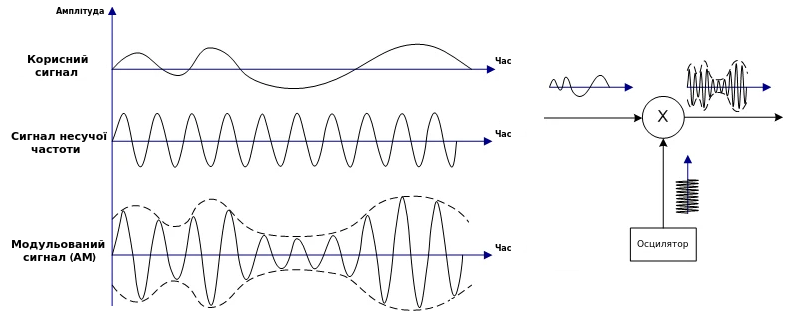
\includegraphics[width=0.9\linewidth]{images/modulation_signal.png}
	\caption{\label{fig:modulation_signal} Модуляція сигналу}
\end{figure}

\textbf{Демодуляція} --- це процес вилучення оригінального інформаційного корисного сигналу з модульованої несучої хвилі. Демодуляція є основною функцією всіх радіоприймачів, телевізорів та комунікаційних приймачів. 
Вцілому модуляція ділиться на два типи: аналогова та цифрова і тут варто пояснити принципову різницю між ними.

В рамках цього блоку ми розглянемо лише базові типи аналоговихта цифривоих модуляцій \footnote{Детальніше питання базових типів модуляцій розкрито у відео, яке можна \href{https://www.youtube.com/watch?v=gfz1FbIOMbs}{переглянути за посиланням}.}. Більш складні типи модуляції --- це по суті комбінація базових типів, розуміючи їх, відносно легко розібратися з іншими.


\subsection{Аналогова модуляція}
\textbf{Аналогова модуляція} --- це процес передачі аналогового низькочастотного базового сигналу через високочастотний несучий аналоговий сигнал. В аналоговій модуляції, як несучий, так і інформаційний, він же корисний сигнал, є аналоговими хвилями. Передача інформації в аналоговій модуляції виконується за рахунок зміни характеристики одного із параметрів, а саме амплітуди, фази або частоти, але також існують і комбінації зі змін цих характеристик.

\subsubsection{Амплітудна модуляція}
\textbf{Амплітудна модуляція} (АМ) --- це метод модуляції, що використовується для передачі інформації шляхом зміни амплітуди сигналу-носія відповідно до миттєвого значення сигналу повідомлення (мал. \ref{fig:am}).

\begin{figure}[h!]
\centering
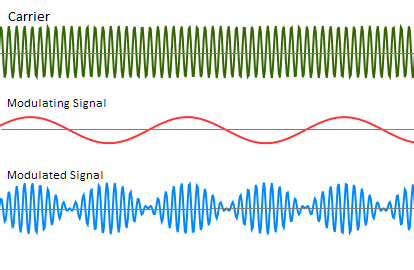
\includegraphics[width=0.6\linewidth]{images/am.png}
\caption{\label{fig:am}Амплітудна модуляція.}
\end{figure}

\begin{itemize}[noitemsep, topsep=8pt]
\item \textbf{Сигнал-носій}: Це високочастотний сигнал постійної амплітуди, частота якого не змінюється під час передачі інформації. Позначений зеленим.
\item \textbf{Модулюючий сигнал}: Це інформаційний сигнал, який несе корисну інформацію (наприклад, керування дроном). Він має відносно низьку частоту порівняно з сигналом-носієм. Позначений червоним.
\item \textbf{Процес модуляції}: Амплітуда сигналу-носія змінюється залежно від амплітуди модулюючого сигналу. Чим вища амплітуда модулюючого сигналу, тим більше змінюється амплітуда носія.
\end{itemize}

\newpage
\subsubsection{Частотна модуляція}

\textbf{Частотна модуляція} (FM) --- це метод модуляції, при якому частота сигналу-носія змінюється відповідно до амплітуди модулюючого сигналу (інформаційного сигналу). Іншими словами, в процесі частотної модуляції амплітуда сигналу-носія залишається незмінною, а частота коливається залежно від миттєвого значення інформаційного сигналу (мал. \ref{fig:fm}).

\begin{figure}[h!]
\centering
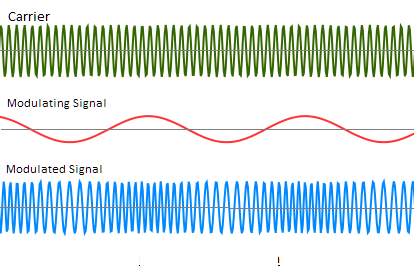
\includegraphics[width=0.6\linewidth]{images/fm.png}
\caption{\label{fig:fm}Частотна модуляція.}
\end{figure}

\begin{itemize}[noitemsep, topsep=8pt]
\item \textbf{Сигнал-носій}: Це високочастотний сигнал, частота якого змінюється в процесі модуляції, але амплітуда залишається постійною. Позн. зеленим.
\item \textbf{Модулюючий сигнал}: Це сигнал, який несе інформацію (наприклад, аудіо). Його амплітуда визначає, на скільки зміниться частота сигналу-носія. Позн. червоним.
\item \textbf{Процес модуляції}: Частота сигналу-носія збільшується, коли амплітуда модулюючого сигналу зростає, і зменшується, коли амплітуда падає. Це відхилення частоти називається \textit{девіацією частоти}.
\end{itemize}

\subsubsection{Фазова модуляція}

\textbf{Фазова модуляція} (PM) --- це метод модуляції, при якому фаза сигналу-носія змінюється відповідно до амплітуди модулюючого сигналу (інформаційного сигналу). На відміну від амплітудної або частотної модуляції, в фазовій модуляції основним параметром, що змінюється, є фаза сигналу(мал. \ref{fig:pm}).

\begin{figure}[h!]
\centering
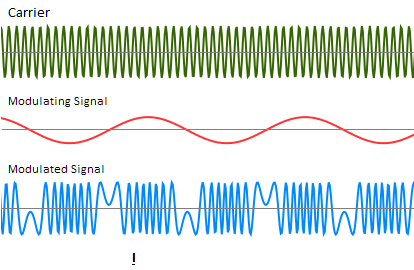
\includegraphics[width=0.6\linewidth]{images/pm.png}
\caption{\label{fig:pm}Фазова модуляція.}
\end{figure}

\begin{itemize}[noitemsep, topsep=8pt]
\item \textbf{Сигнал-носій}: Це високочастотний сигнал, фаза якого змінюється в процесі модуляції, тоді як частота і амплітуда залишаються постійними. Позначений зеленим.
\item \textbf{Модулюючий сигнал}: Це інформаційний сигнал, амплітуда якого визначає, наскільки змінюється фаза сигналу-носія. Позначений червоним.
\item \textbf{Процес модуляції}: Коли амплітуда модулюючого сигналу змінюється, фаза сигналу-носія також змінюється пропорційно до цієї амплітуди. Зміна фази може бути прямою або від'ємною залежно від того, як змінюється модулюючий сигнал.
\end{itemize}

\newpage
\subsection{Цифрова модуляція}
\textbf{Цифрова модуляція} --- це процес передачі цифрового низькочастотного базового сигналу через високочастотний несучий аналоговий сигнал. Цифрова модуляція дещо схожа на аналогову модуляцію, за винятком того, що сигнал базової смуги має дискретний рівень амплітуди. Для двійкового сигналу він має лише два рівні: високий тобто логічна 1, або низький - логічний 0. Відповідно для цифрового сигналу ми робимо трансформацію корисної інформації в двійкові значення 1 та 0 і потім вже робимо модулювання цифрового сигналу на несучий аналоговий сигнал. Тут також варто пояснити, що є модуляція і маніпуляція. Фактично, обидва терміни стосуються одного й того ж процесу, але з деякими відмінностями. Концепція модуляції використовується для аналогових сигналів, а маніпуляції – для дискретних сигналів.

\subsubsection{Амплітудна маніпуляція}
\textbf{Амплітудна маніпуляція}(ASK) --- це техніка, за якої амплітуда несучої хвилі змінюється відповідно до переданих цифрових даних. Частота та фаза залишаються постійними, змінюється лише амплітуда. 

\begin{figure}[h!]
	\centering
	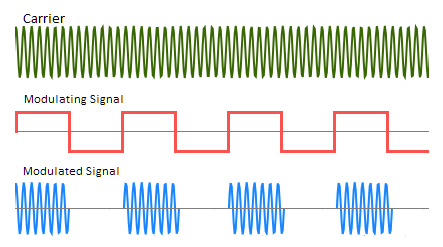
\includegraphics[width=0.6\linewidth]{images/ask.png}
	\caption{\label{fig:ask}Амплітунда маніпуляція.}
\end{figure}


\subsubsection{Частотна маніпуляція}
\textbf{Частотна маніпуляція}(FSK) --- це метод цифрової модуляції, при якому частота несучого сигналу змінюється відповідно до переданих бітів. Амплітуда і фаза залишаються сталими. Це більш надійний метод у шумових середовищах порівняно з амплітудною маніпуляцією.

\begin{figure}[h!]
	\centering
	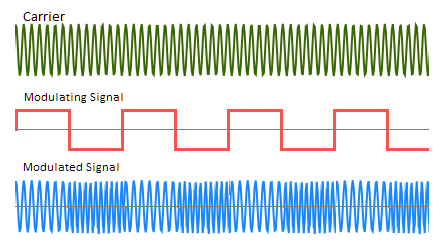
\includegraphics[width=0.6\linewidth]{images/fsk.png}
	\caption{\label{fig:fsk}Частотна маніпуляція.}
\end{figure}

\subsubsection{Фазова маніпуляція}
\textbf{Фазова маніпуляція}(PSK) --- це метод цифрової модуляції, при якому фаза несучого сигналу змінюється залежно від переданих бітів. Амплітуда та частота при цьому залишаються сталими. Цей тип маніпуляції потребує точної синхронізації фаз між передавачем та приймачем, але він є і більш ефективний з точки зору пропускної здатності, ніж ASK або FSK.

\begin{figure}[h!]
	\centering
	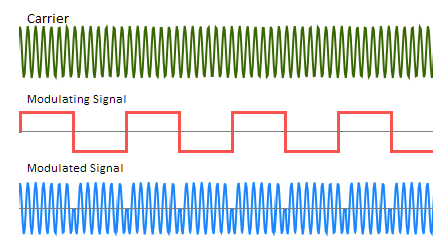
\includegraphics[width=0.6\linewidth]{images/psk.png}
	\caption{\label{fig:psk}Фазова маніпуляція.}
\end{figure}

Три основні методи цифрової модуляції: ASK, FSK та PSK можуть бути використані для передачі одного біта даних (0 або 1) за одиницю часу передачі. Цей метод називається двійковою маніпуляцією зі зсувом (B-ASK, B-FSK або B-PSK). Але оскільки несуча частота є обмеженим ресурсом, метод модуляції кількох бітів в одному часовому інтервалі часто є більш вигідним. У цьому методі кілька бітів даних групуються разом і кодуються в символи. Кожен символ призначається певному рівню модуляції. Ми називаємо ці схеми багаторівневою модуляцією. Якщо згрупувати біти по два, то кожен символ містить по 2 біти. Якщо до символу вдається маніпуляція, результуюча швидкість передачі даних подвоюється, і тоді ми маємо чотири різні символи: 00, 01, 10 та 11 (наприклад 4-PSK або 4-ASK). Якщо згрупувати бітовий потік по чотири, то ми маємо 16 різних символів: 0000, 0001, 0010… до 1111 (наприклад 16-QAM). Все це визначає швидкість передачі даних, яку також називають бітовою швидкістю (бітів за секунду або біт/с). Ми можемо спробувати ще більше збільшити бітову швидкість, але чим складніші символи, тим важче їх розрізняти на стороні приймача.

\begin{figure}[h!]
	\centering
	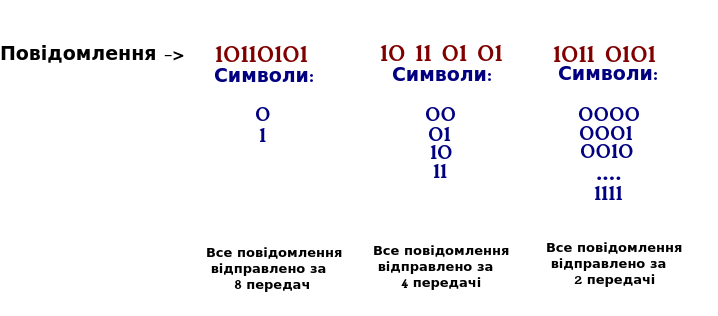
\includegraphics[width=0.8\linewidth]{images/transmittion_speed.png}
	\caption{\label{fig:transmittion_speed} Передача даних в залежності від бітрейту.}
\end{figure}

\begin{figure}[h!]
	\centering
	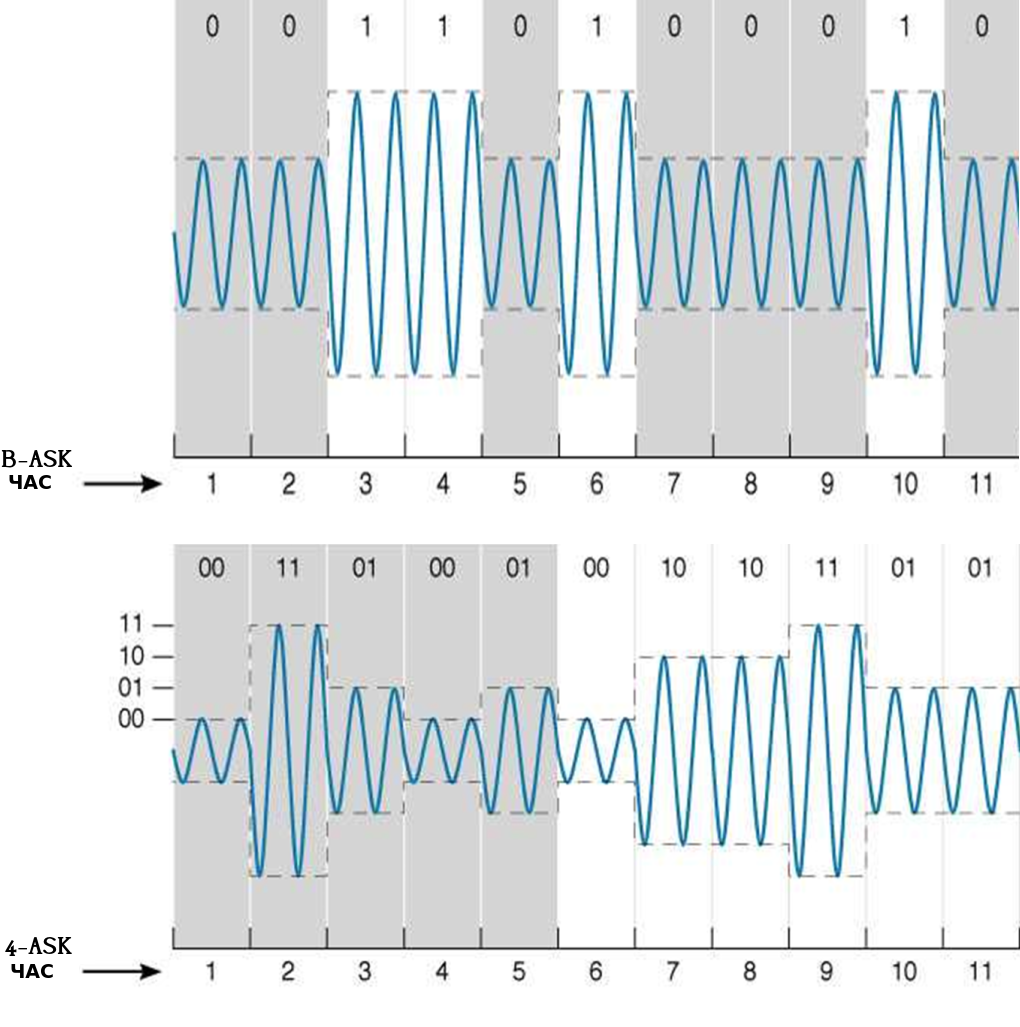
\includegraphics[width=0.7\linewidth]{images/comparison-bask-vs-4ask.png}
	\caption{\label{fig:comparison-bask-vs-4ask} Порівняння передачі данних для B-ASK та 4-ASK.}
\end{figure}


\newpage
\subsubsection{Квадратнурна амплітудна маніпуляція}
\textbf{Квадратнурна амплітудна маніпуляція}(QAM) --- це метод маніпуляції, який поєднує дві несучі хвилі, кожна з різною амплітудою та фазою, але з однією частотою для ефективної передачі даних. Визначення QAM полягає в кодуванні цифрових даних в аналогові сигнали, що дозволяє ефективно передавати інформацію по каналах зв'язку. Цей метод модуляції, який одночасно змінює амплітуду двох несучих хвиль, що знаходяться протифазі на 90 градусів. Таке поєднання амплітудної та фазової модуляції робить QAM особливо потужною, оскільки вона може представляти кілька бітів інформації на символ, збільшуючи пропускну здатність даних. Цей тип модулії також відносно необмежений по бітрейту, тому інсуюють різні різновиди QAM, наприклад: QAM-4 (2 біта), QAM-8(3 біта), QAM-16(4 біта), QAM-64 (6 бітів) і т.д.

\begin{figure}[h!]
	\centering
	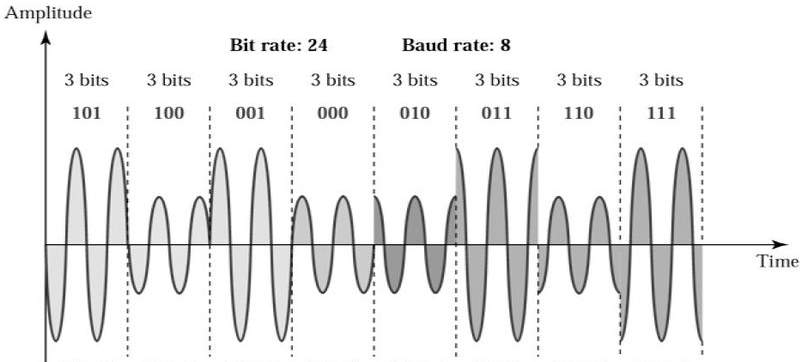
\includegraphics[width=0.7\linewidth]{images/qam.png}
	\caption{\label{fig:qam} QAM-8 модуляція.}
\end{figure}

\newpage
\subsection{Ортогональне частотне мультиплексування}
\textbf{Ортогональне частотне мультиплексування} (OFDM): OFDM – це метод цифрової модуляції, який розділяє доступну смугу частот на кілька ортогональних піднесучих, кожна з яких модульована з низькою швидкістю передачі даних, що дозволяє ефективно передавати сигнали з високою швидкістю передачі даних у багатопроменевому середовищі.
Ортогональні сигнали – це сигнали, перпендикулярні один до одного. Основною властивістю ортогональних сигналів є те, що вони не перешкоджають один одному. Для роботи OFDM потрібна дуже точна синхронізація між вузлами, що здійснюють зв'язок. Якщо в підпотоках виникає відхилення частоти, вони більше не будуть ортогональними, через що виникатимуть інтерференції між сигналами. Це можно уявити собі як паралельну передачу багатьох низькошвидкісних сигналів на різних частотах — разом вони утворюють високошвидкісний канал передачі даних.

\begin{figure}[h!]
	\centering
	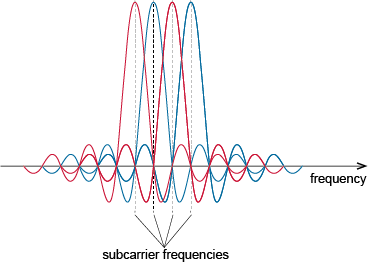
\includegraphics[width=0.7\linewidth]{images/ofdm.png}
	\caption{\label{fig:ofdm}  Приклад OFDM.}
\end{figure}


\subsection{ППРЧ}

\textbf{ППРЧ} (Перестроювання по частоті із псевдовипадковою перебудовою частоти) -- це метод радіозв'язку, при якому частота передавача змінюється за певним законом, зазвичай у псевдовипадковій послідовності. Така техніка використовується для підвищення стійкості зв'язку до перешкод, запобігання перехопленню, а також для кращого використання спектра.

Основна ідея ППРЧ полягає в тому, що передавач і приймач узгоджено \textit{перестрибують} між частотами в заздалегідь визначеному порядку. Якщо сторонній слухач не знає цієї послідовності, він не зможе прийняти корисний сигнал.

\begin{figure}[H]
\centering
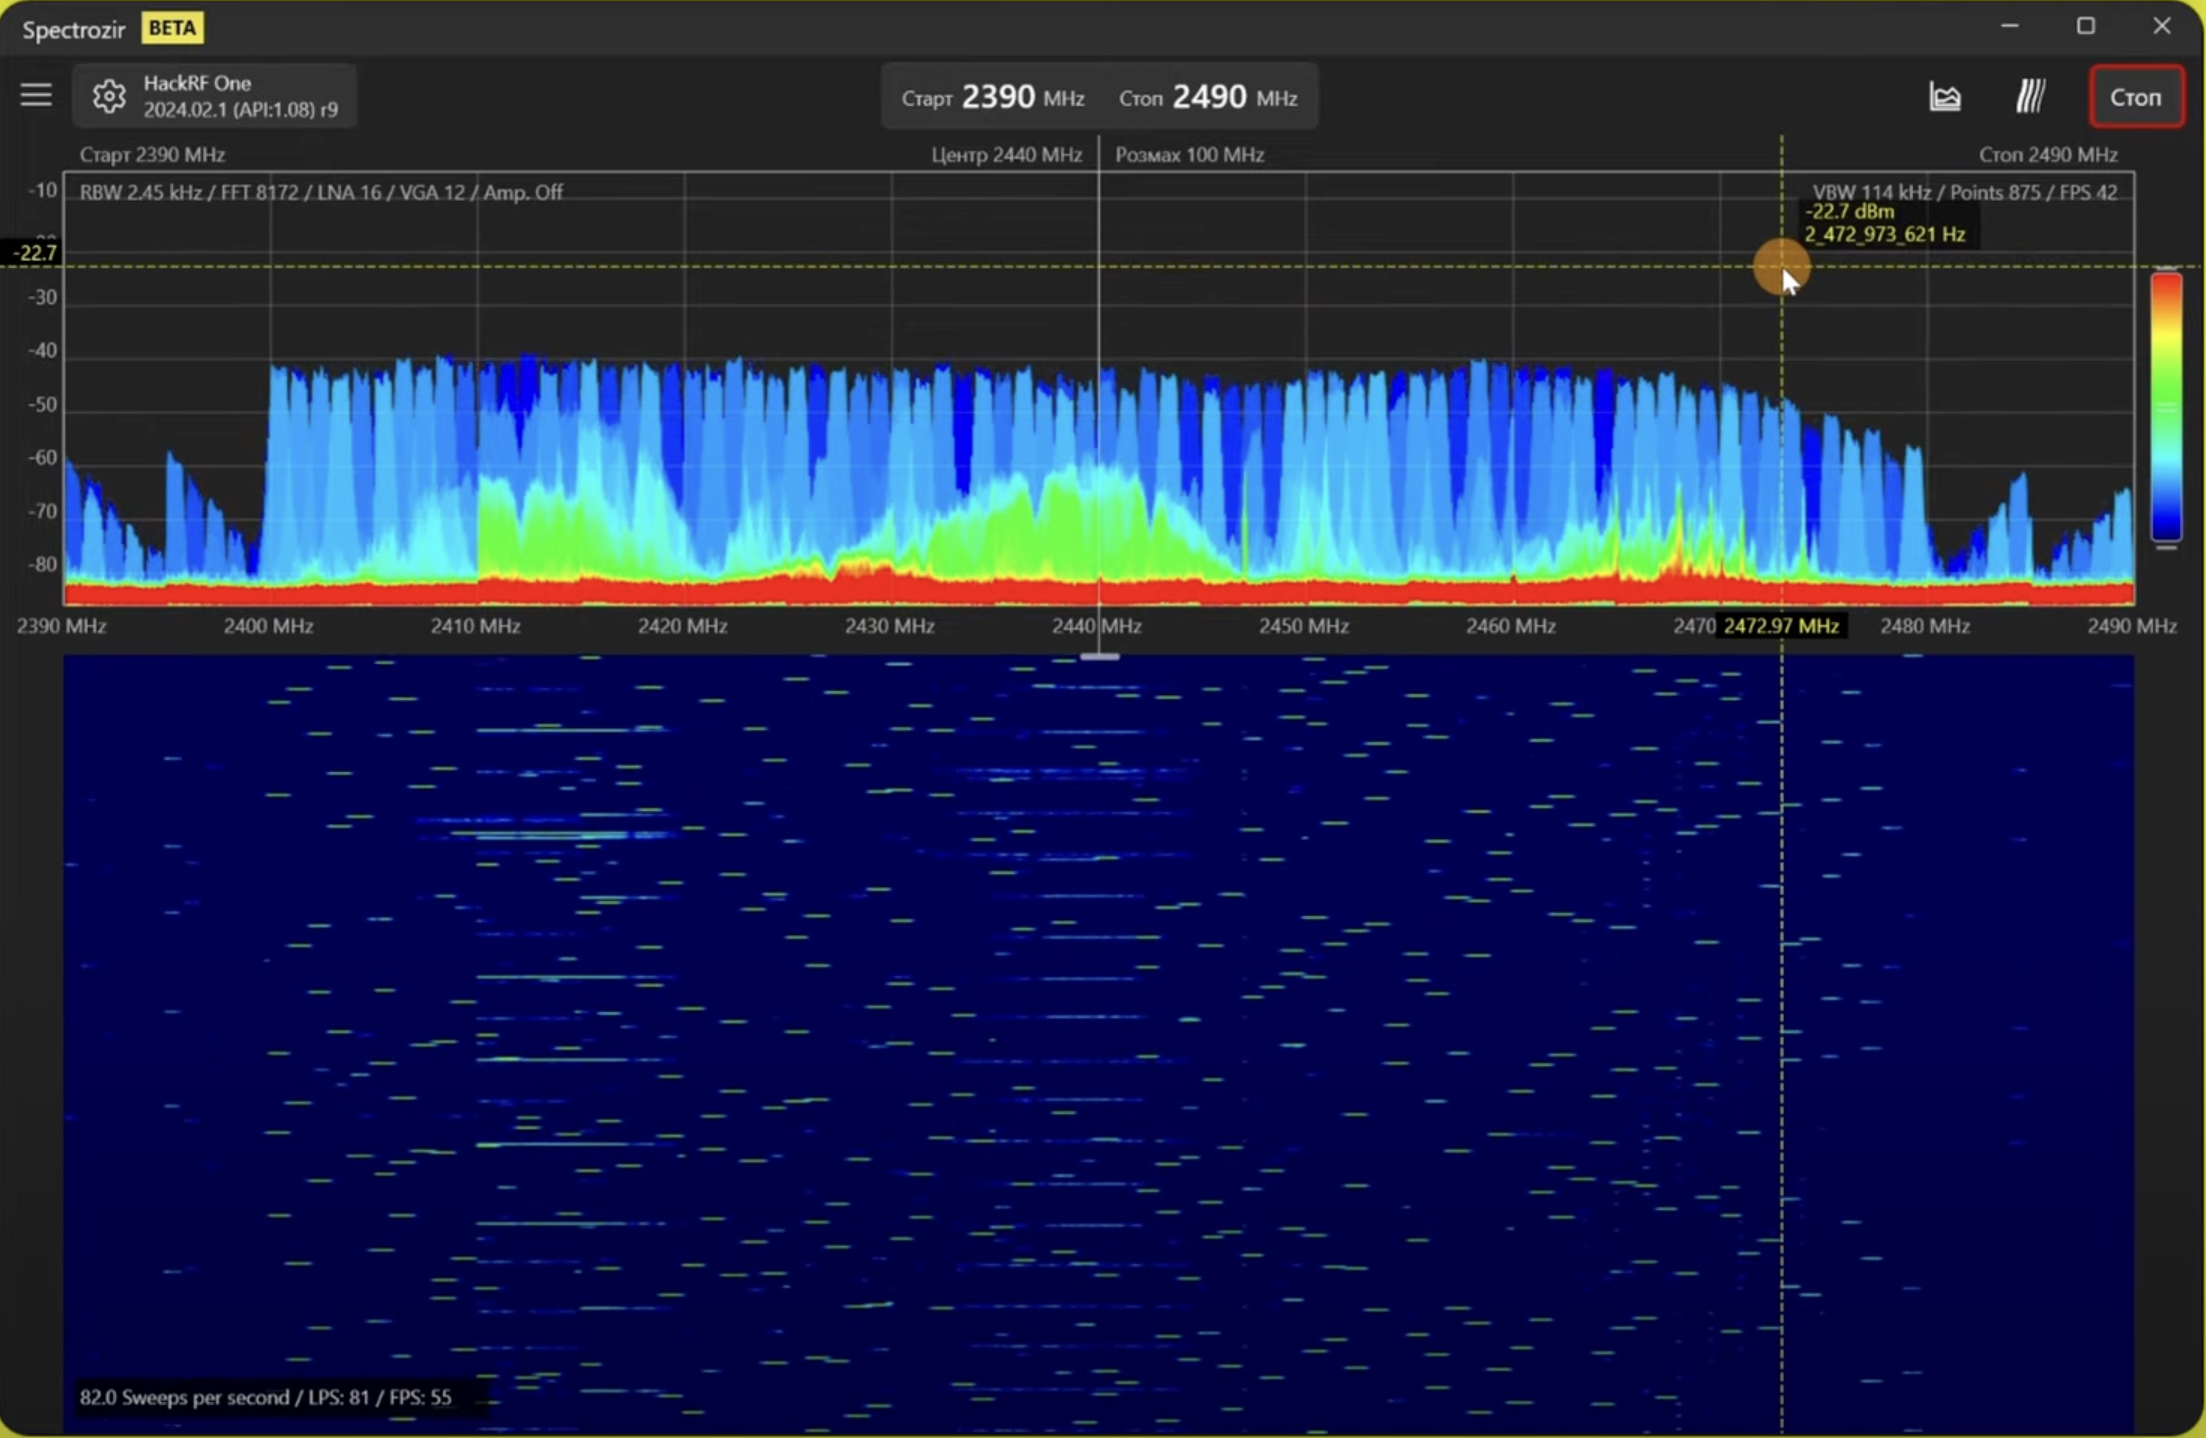
\includegraphics[width=0.7\linewidth]{images/freq-hope.png}
\caption{\label{fig:hf}ППРЧ радіо сигналу протоколу ELRS на частоті 2.4ГГц.}
\end{figure}

Технологія ППРЧ знайшла широке застосування у протоколах керування дронами (сигнал йде від пульта до БПЛА) через властивості такого методу передачі:
\begin{itemize}[noitemsep, topsep=8pt]
\item \textbf{Стійкість до перешкод}: Сигнал на кожній окремій частоті передається протягом короткого періоду часу, що робить його важче заглушити.
\item \textbf{Ефективність спектра}: Покращує ефективність використання радіочастотного спектра, оскільки сигнал розподіляється по різних частотах.
\end{itemize}

Якщо дуже спрощено, то сигнали керування від пульта (фактичні дії оператора) перетворюються на окремі пакети, які передаються по радіоканалах на певній смузі у псевдовипадковому режимі. Для того щоб подавити такий сигнал, потрібно створювати заваду не на окремих каналах передачі, а по всій смузі частот. Більше детально, як виглядає ППРЧ, можна \href{https://www.youtube.com/watch?v=REyNJcrZHII}{подивитись у відео за посиланням}.

\subsection{LORA}
\textbf{LORA} --- це технологія, яка була розроблена для застосувань з великим радіусом дії та низьким енергоспоживанням і знайшла своє застосування в цивільному житті для IOT, але вона себе також знайшла і у віськововій галузі. Серед військових LORA використовує в протоколах TBS та ELRS для коммунікації між пультом та FPV дроном. Тут варто зазначити, що LORA в цьому випадку це саме фізичний рівень та метод за яким відбувається модуляція. Метод модуляції LORA побудований на базі чірпу (CSS -  Chirp Spread Spectrum), стійкий до перешкод та багатопроменевих згасань. Chirp Spread Spectrum розшифровується як «стиснутий високоінтенсивний радарний імпульс» і представляє собою спеціалізований тип модуляції FSK. Це сигнал, частота якого з часом або збільшується (Up Chirp), або зменшується(Down Chirp). LoRa має 6 (SP - speading factors) коефіцієнтів розширення (SF7 - SF12) та три різні пропускні смуги (125 кГц, 250 кГц та 500 кГц). Торкаючись теми спред фактору(SF) ми повинні розуміти, що кожен наступний SF зазвичай буде вдвічі більше по часу за попердній, окрім SF7, тому що він є першим в цьому ланцюжку. Тобто, SF8 займає вдвічі більше часу, ніж SF7, а SF9 займає вдвічі більше часу, ніж SF8 і т.д. Символи LoRa модулюються по висхідному частотному сигналу смуги  і використовуються різні ортогональні коефіцієнти розширення залежно від вимог до швидкості передачі даних та умов каналу. Вищий коефіцієнт розширення (SF) - більший час передачі даних, нижчий коефіцієнт розширення - вища швидкість передачі даних.

\begin{figure}[h!]
	\centering
	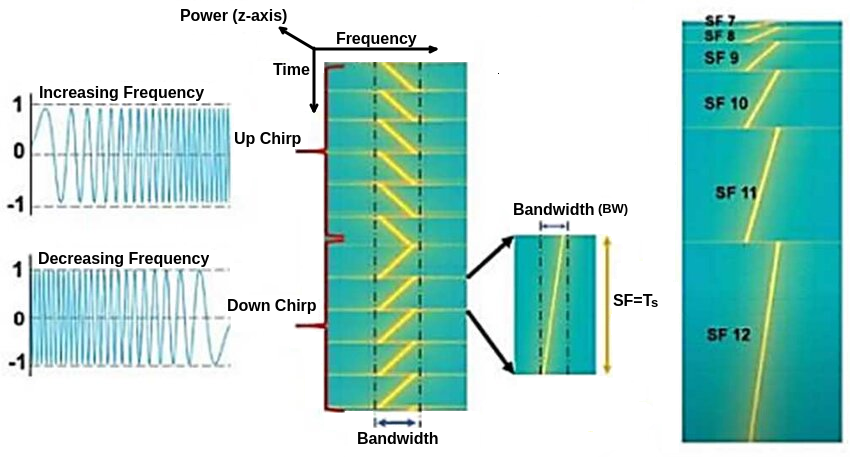
\includegraphics[width=0.9\linewidth]{images/lora_chirp_main.png}
	\caption{\label{fig:lora_chirp_main} Загальний огляд пакету LORA}
\end{figure}

Співвідношення швидкості передачі символів (Ts) в секунду визначається за формулою:

\[
T_s = \frac{\mathrm{BW}}{2^{\mathrm{SF}}}
\]

\begin{itemize}[noitemsep, topsep=8pt]
	\item ${BW}$ -- ширина пакету в Hz
	\item ${SF}$ -- коефіцієнт розширення  
	\item ${Ts}$ -- тривалість символа в секундах
\end{itemize}
Звідси можно визначити формулу розрахунку спредінг фактору (SF):

\[
{2^{\mathrm{SF}}} = {\mathrm{BW}}*{\mathrm{T_s}}
\]

Структура пакету LORA включає в себе преамбулу, яка зазвичай складає 8 символів, але може бути і іншою, бо є можливість їх міняти, 2-2.5 символів синхронізації (в протилежному напрямку), які використовуються для синхронізації часу і відповідно решти пакету - корисної інформації, тобто модульованих символів.

\begin{figure}[h!]
	\centering
	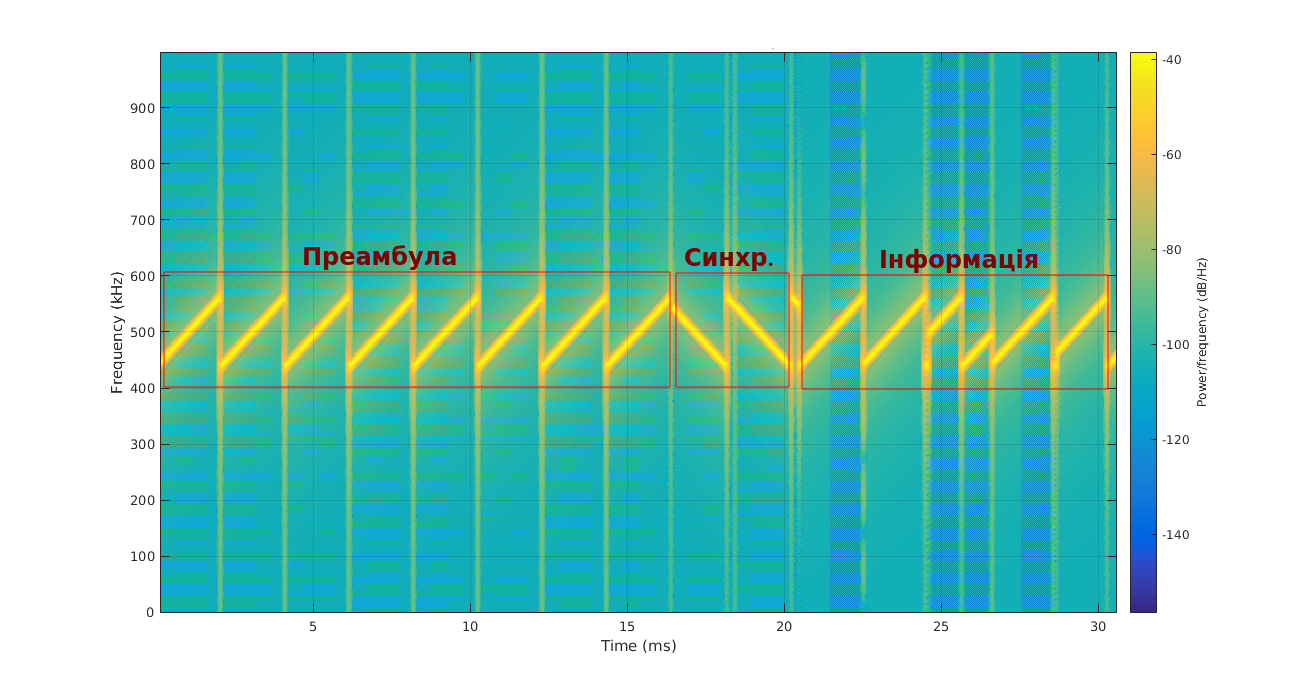
\includegraphics[width=0.8\linewidth]{images/lora_preambul.png}
	\caption{\label{fig:lora_preambul} Структура пакету LORA}
\end{figure}


\newpage
\section{Спектральний аналіз}

Щоб зрозуміти, що таке спектральний аналіз, нагадаю про важливі властивості хвиль --- ми можемо взяти декілька сигналів (позначені синім) і просумувати їх в один фінальний сигнал (позначений червоним), тим самим отримавши комплексний сигнал. Таким чином працює модуляція (див. секцію \ref{sec:modulation}).

\begin{figure}[h!]
\centering
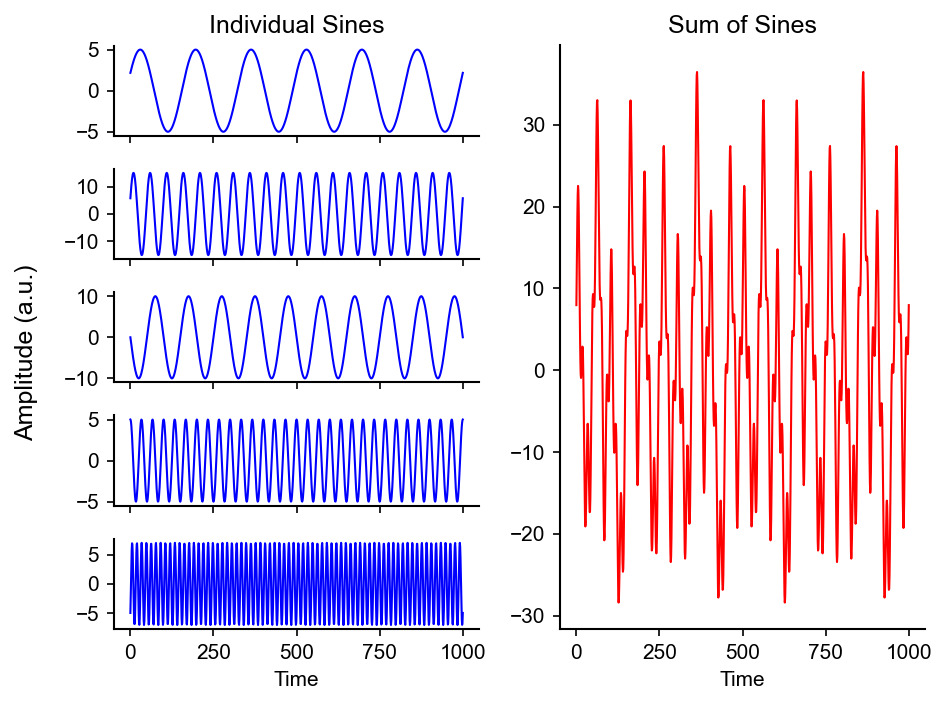
\includegraphics[width=0.6\linewidth]{images/signals-sum.png}
\caption{\label{fig:signals-sum}Процес формування \textit{складного} сигналу шляхом складання декількох окремих сигналів.}
\end{figure}

Цю процедуру можна зробити і в зворотньому напрямку --- отримавши сигнал із радіоефіру, застосовуючи певні алгоритми\footnote{Для розкладання сигналу на складові виконується обробка сигналу під назвою \textit{швидке перетворення Фур'є} (FFT)}, розкласти його на складові. Кожна складова — це синусоїдальний сигнал зі своєю частотою. Таким чином ми можемо відобразити складові на окремому графіку, тим самим відобразивши сигнал у \textbf{частотній області} (або ще можна зустріти термін \textbf{частотний домен}\footnote{Тема частотного домену і перетворення Фур'є дуже цікава, але обширна. Більш поглиблено про це можна почитати в \href{https://pysdr.org/ukraine/content-ukraine/frequency_domain.html}{інших джерелах}.}). На малюнку \ref{fig:freq-domain} частотна область зображена голубим кольором. Цей графік дає нам можливість зрозуміти, які складові присутні у сигналі на певному діапазоні частот.

\begin{figure}[h!]
\centering
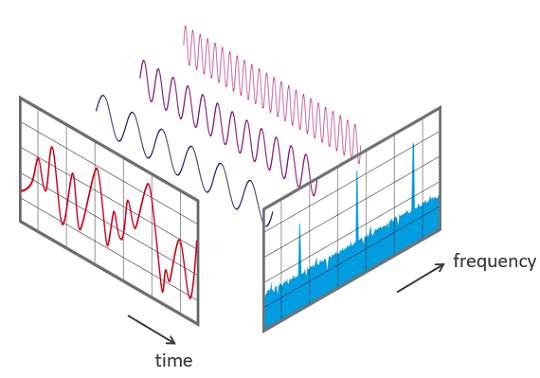
\includegraphics[width=0.7\linewidth]{images/freq-domain.png}
\caption{\label{fig:freq-domain}Розкладання сигналу на складові або перевід сигналу з часової у частотну область.}
\end{figure}

Відображення сигналу у частотній області відповідає певному проміжку часу. Наприклад, ми записуємо сигнал із радіоефіру тривалістю \texttt{0.1c} з діапазоном частот від \texttt{500MГц -- 1ГГц} і будуємо для нього відображення у частотній області. Якщо ми повторимо цю процедуру, скажімо, \texttt{100} разів, то отримаємо \texttt{100} графіків у частотній області, які відповідають одному й тому самому діапазону, але кожен окремо відображає свій проміжок часу. Тепер, якщо ми їх складемо, то отримаємо картину того, як сигнал (а саме його складові) змінювався у часі. Це те, що ми бачимо на екрані спектроаналізатора.

\begin{figure}[h!]
\centering
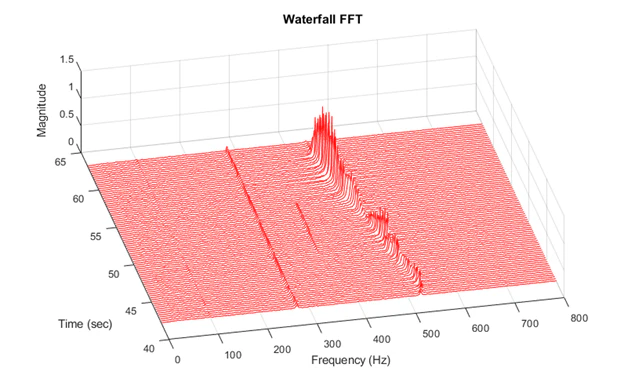
\includegraphics[width=0.75\linewidth]{images/fft-stack.png}
\caption{\label{fig:fft-stack}FFT перетворення складені у стек.}
\end{figure}

Опціонально, можна накласти \textit{тепловий градієнт} на графік, підсвічуючи гарячим області з більшою амплітудою сигналу\footnote{Майже кожен тип модуляції має свій характерний малюнок на водоспаді. Знаючи їх, можна впізнавати сигнали від БПЛА, перевіряти засоби РЕБ (чи працюють вони на заявлених діапазонах і яка щільність завади). Пристрої, за допомогою яких це можна зробити, називаються \textbf{спектроаналізаторами}.}.

\begin{figure}[H]
    \centering
       \begin{minipage}{0.35\textwidth}
        \centering
        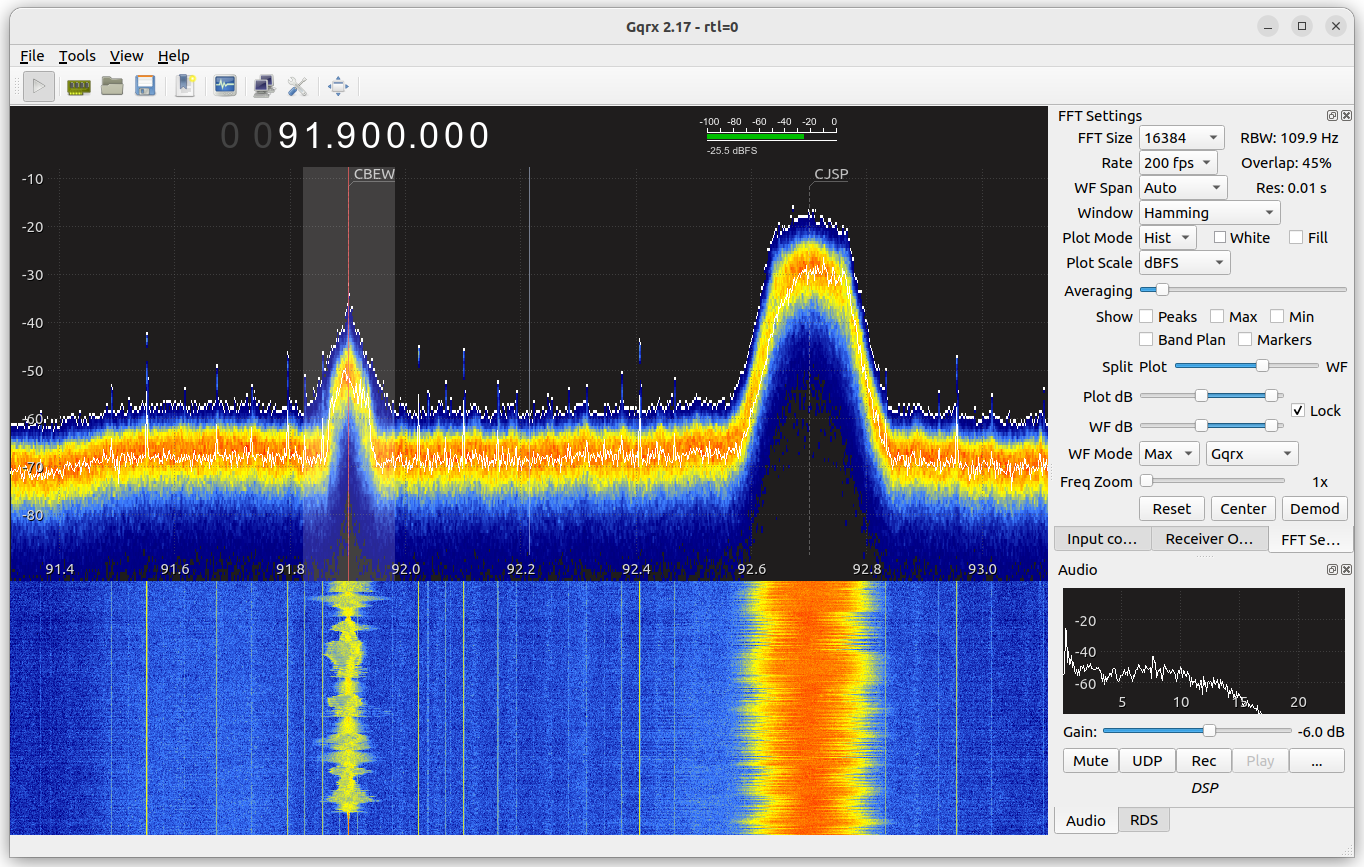
\includegraphics[width=\textwidth]{images/gqrx.png}
    \end{minipage}
    \begin{minipage}{0.55\textwidth}
        \centering
        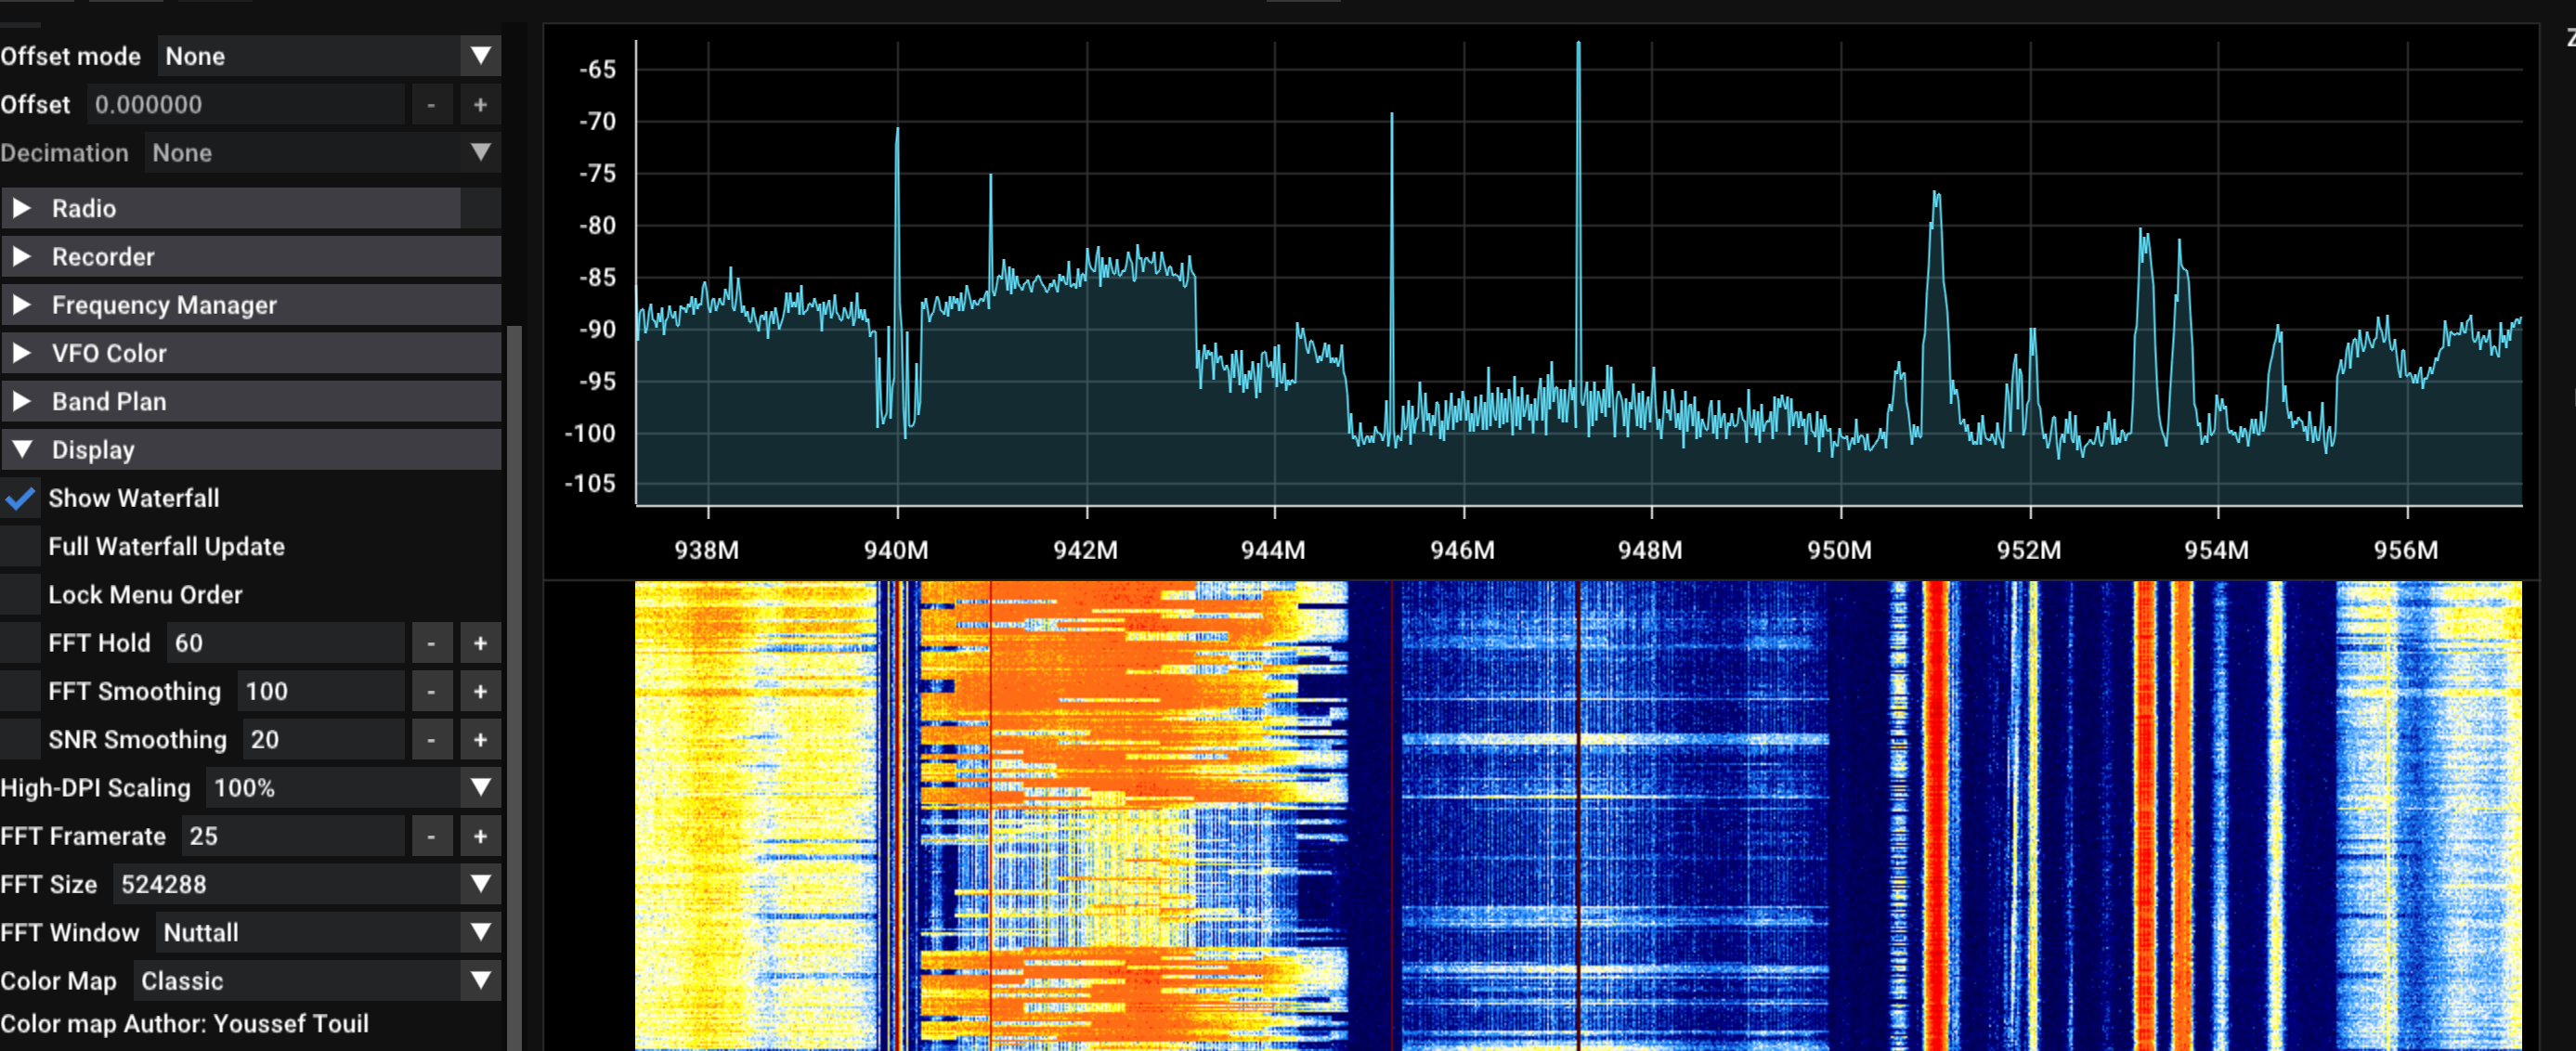
\includegraphics[width=\textwidth]{images/sdrpp.png}
    \end{minipage}
    \caption{Вікно програми GQRX(зліва) і SDR++(справа).}
\end{figure}

\subsection{Обладнання}

Спектроаналізатор --- це тип пристроїв, які мають дуже широку номенклатуру. Вони розрізняються за багатьма параметрами (портативність, частота семплювання, миттєва смуга, розрядність АЦП, тощо), які впливають на вартість приладу. Ціна може починатись від 100\$ і сягати декількох тисяч доларів. В залежності від задачі і бюджету можна підібрати спектроаналізатор під свої потреби.

\begin{figure}[H]
\centering
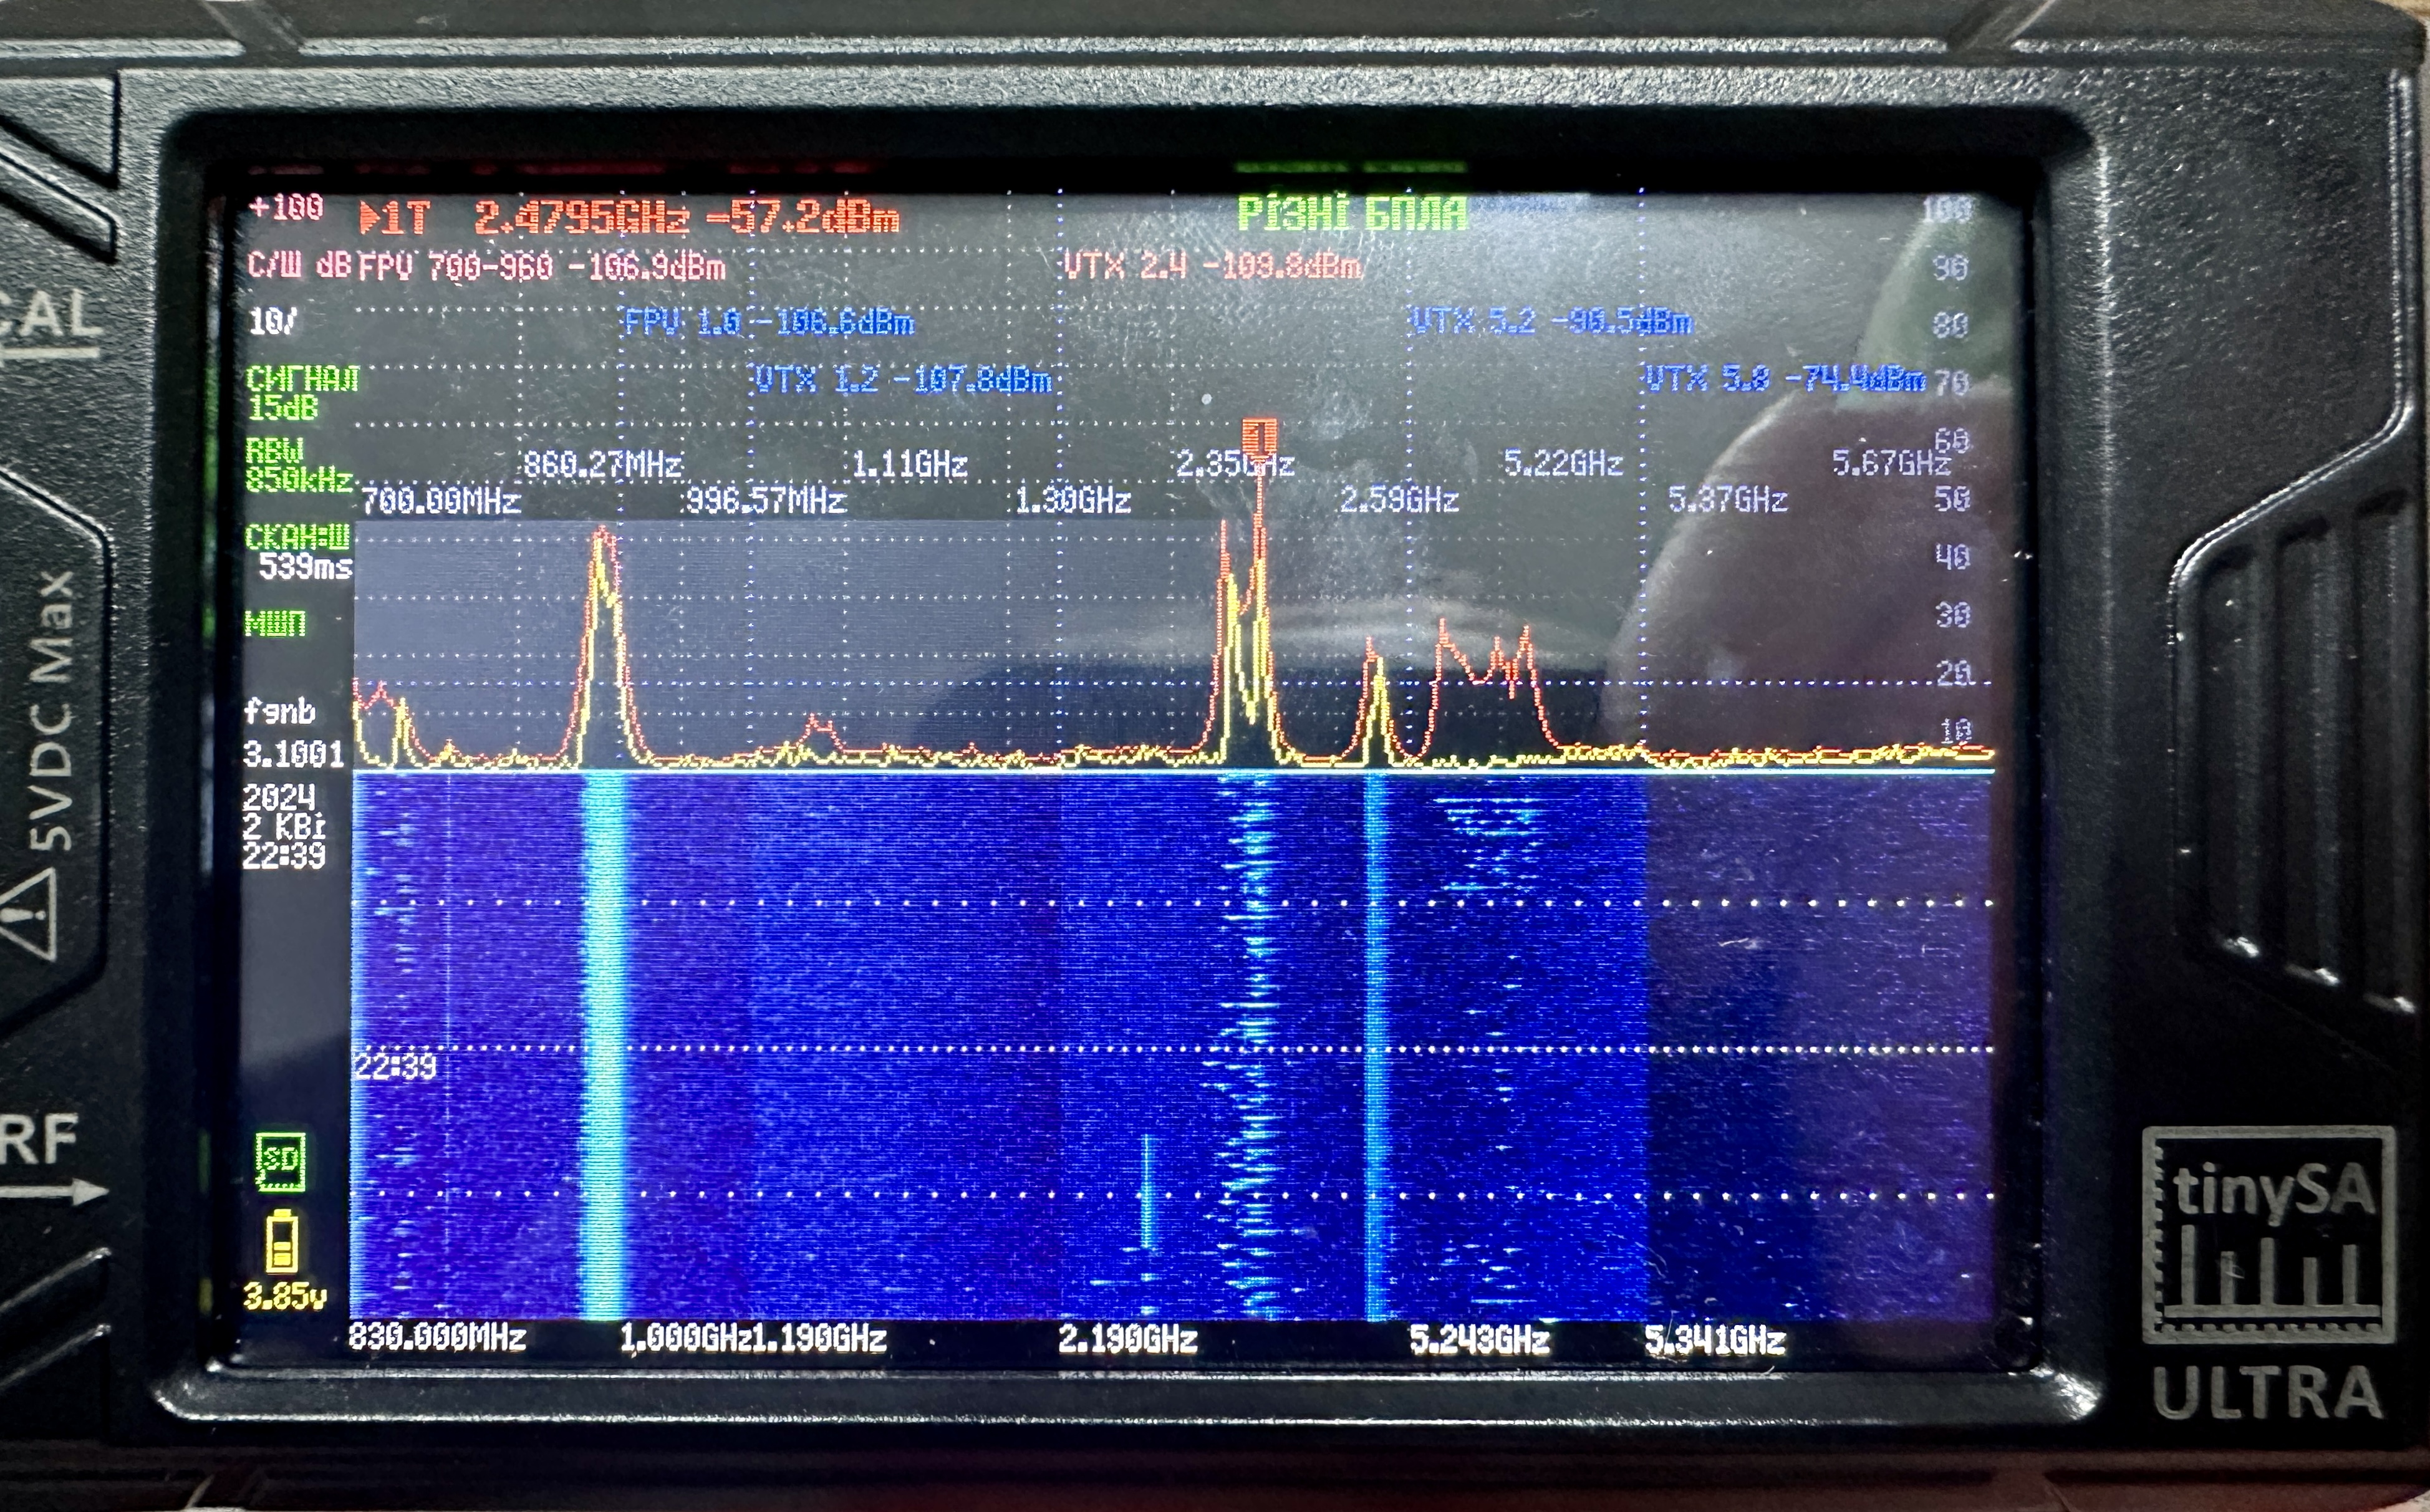
\includegraphics[width=0.7\linewidth]{images/tinysa.jpg}
\caption{\label{fig:tinysa}Портативний спектроаналізатор TinySA Ultra з прошивкою ЗСУ.}
\end{figure}

\textbf{TinySA Ultra} -- портативний спектроаналізатор, який дозволяє робити огляд смуги частот до 6ГГц. Є базові версії і збірки на базі цього пристрою (надрукований корпус на 3D принтері з направленою антеною). Засіб дозволяє:

\begin{itemize}[noitemsep, topsep=8pt]
\item Визначати напрямок сигналу (за допомогою направленої антени), наприклад, відео з FPV дрона.
\item Перевіряти роботу РЕБ шляхом оцінки завади, яка відображається на екрані пристрою.
\item Робити оцінку радіоефіру для розрахунків БпАК (дивитись, які частоти зайняті, щоб уникати перешкод).
\end{itemize}


\textbf{HackRF One} --- це інший клас пристрою початкового рівня, т.н. SDR-приймач. Робочий діапазон також складає до 6ГГц. За допомогою цього засобу можна вирішувати більш складні задачі аналізу, організовувати пост спостереження, записувати т.н. IQ-семпли (дані радіоефіру) для подальшої обробки. Важливо зауважити, що це не пристрій сам в собі, а те, що підключається до робочої станції і потребує додаткового програмного забезпечення\footnote{Перевагою HackRF One є те, що існує багато програмного забезпечення, яке підтримує роботу з цим пристроєм, найбільш відомі: \href{https://airspy.com/download/}{SDR\#}, \href{https://www.sdrpp.org/}{SDR++}, \href{https://www.gqrx.dk/}{GQRX}, \href{https://spectrozir.com/}{Spectorzir}}.

\begin{figure}[H]
    \centering
       \begin{minipage}{0.4\textwidth}
        \centering
        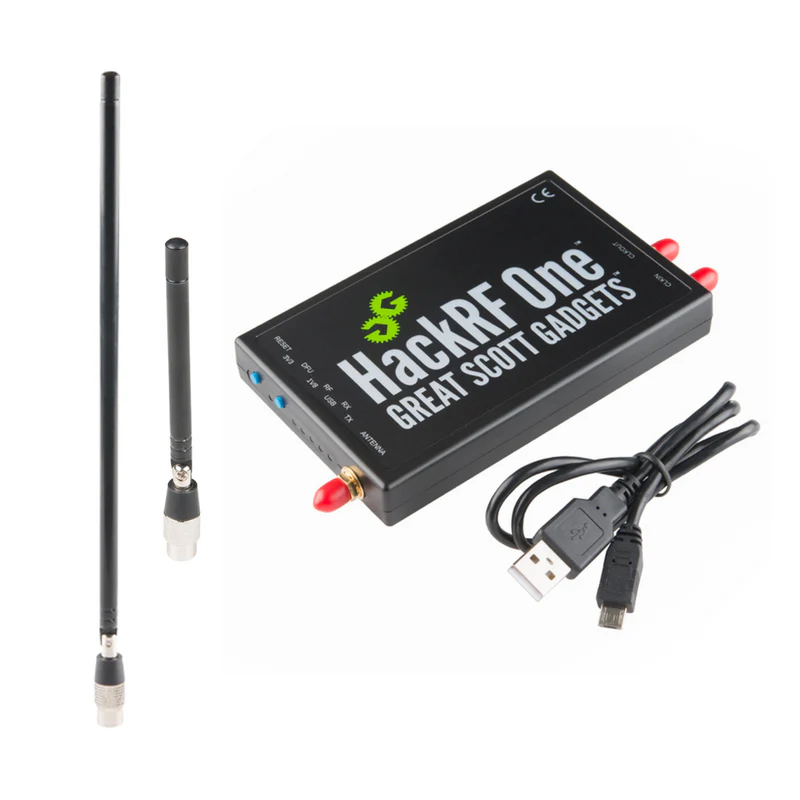
\includegraphics[width=\textwidth]{images/hackrf.png}
    \end{minipage}
    \begin{minipage}{0.3\textwidth}
        \centering
        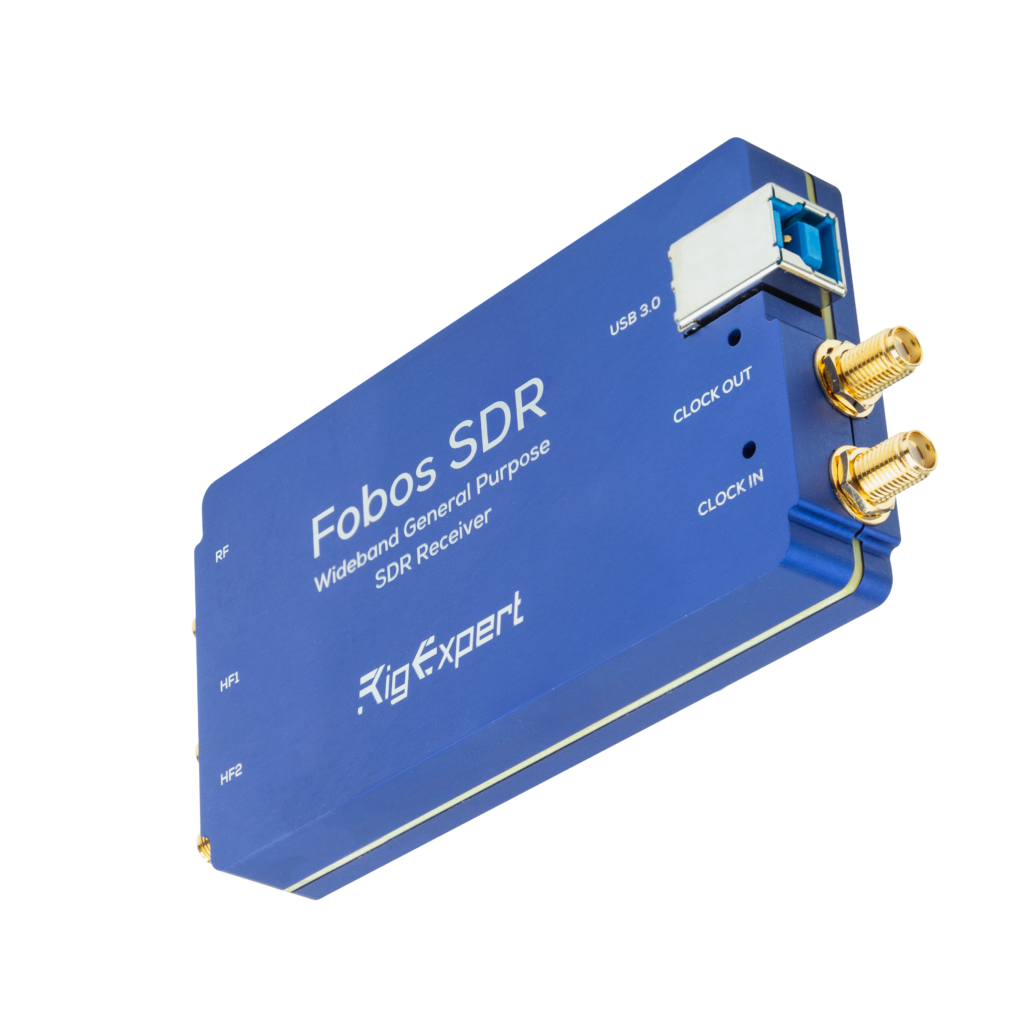
\includegraphics[width=\textwidth]{images/fobos.png}
    \end{minipage}
    \caption{\label{fig:hackrf}Загальний HackrRF One(зліва) і FobosSDR(зправа).}
\end{figure}

\subsection{Додаткові матеріали по темі}

\begin{itemize}[noitemsep, topsep=8pt]
\item \href{https://sprotyvg7.com.ua/lesson/sistemi-radiozvyazku-z-pprch}{Системи радіозв'язку з псевдовипадковим переналаштуванням робочої частоти}.
\item \href{https://www.youtube.com/watch?v=KCj1-SM9aAA}{Порівняння TinySA Base, TinySA Ultra, SA6 (Arinst) та HackRF One}.
\item \href{https://www.youtube.com/watch?v=eFXym8-Yzt0}{Спектр керування FPV на ELRS 915 МГц, знято в екранованій камері на PR200}.
\item \href{https://www.youtube.com/watch?v=REyNJcrZHII}{ELRS 2.4GHz. Як виглядає ППРЧ сигнал радіо протоколу ELRS на частоті 2.4GHz}.
\item \href{https://www.youtube.com/watch?v=XzFMRYEYVXM}{Як виглядає відеосигнал FPV дрона на частоті 5.8 ГГц}.
\end{itemize}

\section{Антени}
\textbf{Антена} --- це пристрій, призначений для передачі або прийому електромагнітних хвиль. Вона перетворює електричні сигнали в радіохвилі при передачі, і радіохвилі в електричні сигнали при прийомі. Далі по тексту, коли буде зустрічатися термін антена, то мається на увазі антена для РЕБ-у. Для РЕБ-у ближньої дії можуть бути використані антени двох типів:

\begin{itemize}[noitemsep, topsep=8pt]
\item \textbf{Направлені} -- мають бути зорієнтовані у напрямку ймовірного маршруту БПЛА.
\item \textbf{Всеспрямовані} -- утворюють т.н. купол навколо засобу РЕБ.
\end{itemize}

\subsection{Діаграма спрямованості}
Антена, що випромінює енергію однаково в усіх напрямках, називається сферичним випромінювачем або ізотропним випромінювачем. Пояснення цього поняття: якщо помістити точкове джерело світла в центр скляної кулі, то її поверхня буде рівномірно освітлена цим джерелом, тобто щільність випромінювання буде однаковою в будь-якій точці поверхні сфери. Однак неможливо створити строго сферичний випромінювач. Він існує лише в теорії і слугує для порівняльних цілей. Жодна реальна антена не здатна забезпечити однакову щільність і поляризацію випромінювання в усіх напрямках. Тому будь-яка антена має певну спрямованість, що описується відповідною діаграмою. Для точного відображення спрямованості необхідно побудувати її тривимірне (просторове) зображення. Однак просторовий розподіл щільності важко відобразити графічно, тому зазвичай обмежуються представленням діаграми спрямованості антени у вертикальній та горизонтальній площинах.

\begin{figure}[H]
\centering
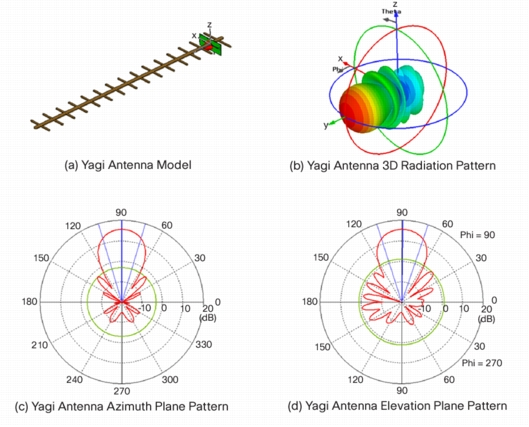
\includegraphics[width=0.6\linewidth]{images/yagi-antenna.jpg}
\caption{\label{fig:yagi:antenna}Діаграма спрямованості з вузькою діаграмою спрямованості.}
\end{figure}

Діаграма спрямованості та підсилення антени взаємопов'язані. Пояснимо їх взаємозв'язок на прикладі скляної кулі. Якщо джерело світла в центрі кулі забезпечити відбивачем (наприклад, параболічним дзеркалом), світло буде йти у вигляді пучка, і випромінювання стане спрямованим. Таким чином, освітленою виявиться лише частина поверхні кулі, обмежена через спрямованість випромінювання. При цьому щільність потоку енергії випромінювання в межах спрямовано освітленої частини поверхні значно перевищить відповідне значення при рівномірному освітленні кулі, оскільки на дану ділянку потраплять також ті промені, які до появи відбивача освітлювали інші частини поверхні. Щільність потоку енергії випромінювання тим вища, чим гостріша спрямованість випромінювання. Тому підсилення за щільністю потоку енергії відносно ізотропного випромінювання прямо залежить від діаграми спрямованості. Як підсилення, так і діаграма спрямованості виражають \textbf{концентрацію випромінювання в певному напрямку}.

\begin{figure}[H]
\centering
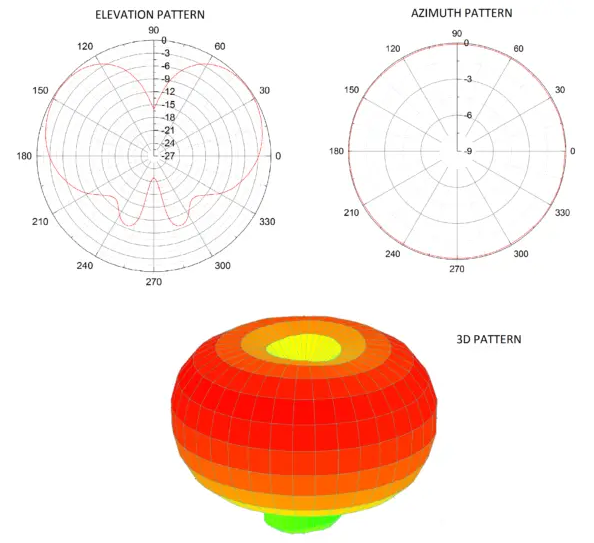
\includegraphics[width=0.5\linewidth]{images/omni-antenna.png}
\caption{\label{fig:omni:antenna}Діаграма спрямованості антени з круговою поляризацією.}
\end{figure}

\subsection{Поляризація антен}

Для електромагнітної хвилі поляризація фактично є площиною, в якій електрична хвиля вібрує. Це важливо при розгляді антен, оскільки вони чутливі до поляризації і зазвичай приймають або передають сигнал лише з певною поляризацією.

Для більшості антен дуже легко визначити поляризацію. Вона просто знаходиться в тій же площині, що і елементи антени. Отже, вертикальна антена (тобто антена з вертикальними елементами) найкраще буде приймати вертикально поляризовані сигнали, а також горизонтальна антена буде приймати горизонтально поляризовані сигнали.

Відповідно, поляризація антен, розташованих у вільному просторі, дуже важлива, і, очевидно, вони повинні знаходитися в однаковій площині, щоб забезпечити оптимальний сигнал. Якби вони знаходились під прямим кутом один до одного (тобто крос-поляризовані), то теоретично сигнал не приймався б, але на практиці, коли у антен (засобу подавлення і на дроні) різні поляризації, то такий засіб \textbf{працювати буде}, але із втратою ефективності (див. Табл. \ref{table:polarization}).

\begin{table}[ht]
\centering
\begin{tabular}{|l|l|l|l|l|l|}
\hline
\textbf{Поляризація / Db} & \textbf{Верт.} & \textbf{Гор.} & \textbf{Під 45°} & \textbf{Право кругова} & \textbf{Ліво кругова} \\
\hline
Вертикальна      & 0           & $\infty$     & 3            & 3            & 3            \\
Горизонтальна    & $\infty$    & 0            & 3            & 3            & 3            \\
Під 45°          & 3           & 3            & 0 або $\infty$ & 3            & 3          \\
Право кругова    & 3           & 3            & 3            & 0            & 3            \\
Ліво кругова     & 3           & 3            & 3            & 3            & 0            \\
\hline
\end{tabular}
\caption{\label{table:polarization}Вплив розташування антен з різним типом поляризації \cite{book:rothammel}.}
\end{table}


\textbf{Приклади}. Для дрона з горизонтальною антеною (горизонтальна поляризація) і засобом подавлення з вертикальною антеною (вертикальна поляризація) типу діполь (штирьова антена) подавлення буде неефективним. Для цього на практиці такого типу антени намагаються розташувати під кутом 45 градусів. Тому виробники якісного РЕБ-у встановлюють антени типу \textit{конюшина}, \textit{діск-конусні}, \textit{квадрифилярні}, тощо, які дають складну поляризацію.

\begin{figure}[H]
\centering
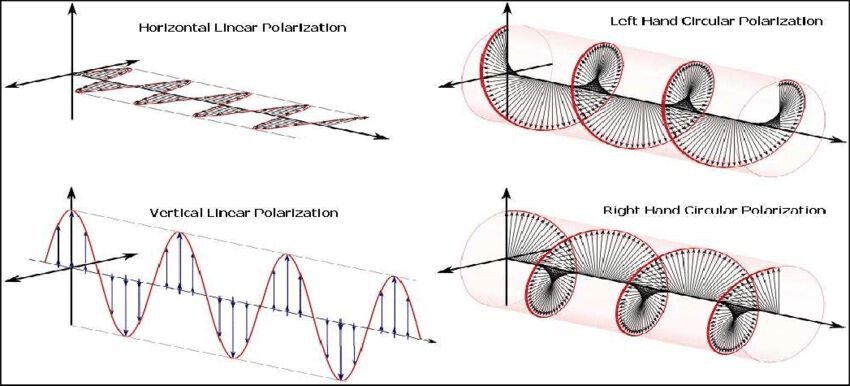
\includegraphics[width=0.7\linewidth]{images/polarization.jpeg}
\caption{\label{fig:polarization}Основні типи поляризацій антен.}
\end{figure}

\subsection{Хвильовий опір антени}
Опір антени, або хвильовий опір антени, це характеристичний параметр антени, який описує, як антена передає або приймає електромагнітні хвилі. Він визначає, як електричні сигнали, що передаються через антену, перетворюються на радіохвилі, і навпаки, як радіохвилі, що приймаються антеною, перетворюються на електричні сигнали. Опір антени складається з двох основних компонентів:

\begin{itemize}[noitemsep, topsep=8pt]
\item \textbf{Активний опір} (омічний опір) --- це частина опору, яка відповідає за перетворення електричної енергії в радіохвилі (випромінювання). Активний опір сприяє випромінюванню сигналу в навколишній простір.
\item \textbf{Реактивний опір} --- це частина опору, яка відповідає за зберігання енергії в електричному або магнітному полях навколо антени. Реактивний опір не сприяє випромінюванню енергії, але може призводити до її втрат у вигляді тепла.
\end{itemize}

Хвильовий опір антени важливий для забезпечення максимальної ефективності передачі енергії від передавача до антени або від антени до приймача. Щоб уникнути відбиття сигналів і забезпечити максимальне випромінювання або прийом сигналу, необхідно, щоб опір антени був узгоджений з хвильовим опором фідера (кабеля), що підключений до антени. Це узгодження відбувається, коли імпеданс (загальний опір) антени дорівнює імпедансу фідера.


\begin{figure}[H]
\centering
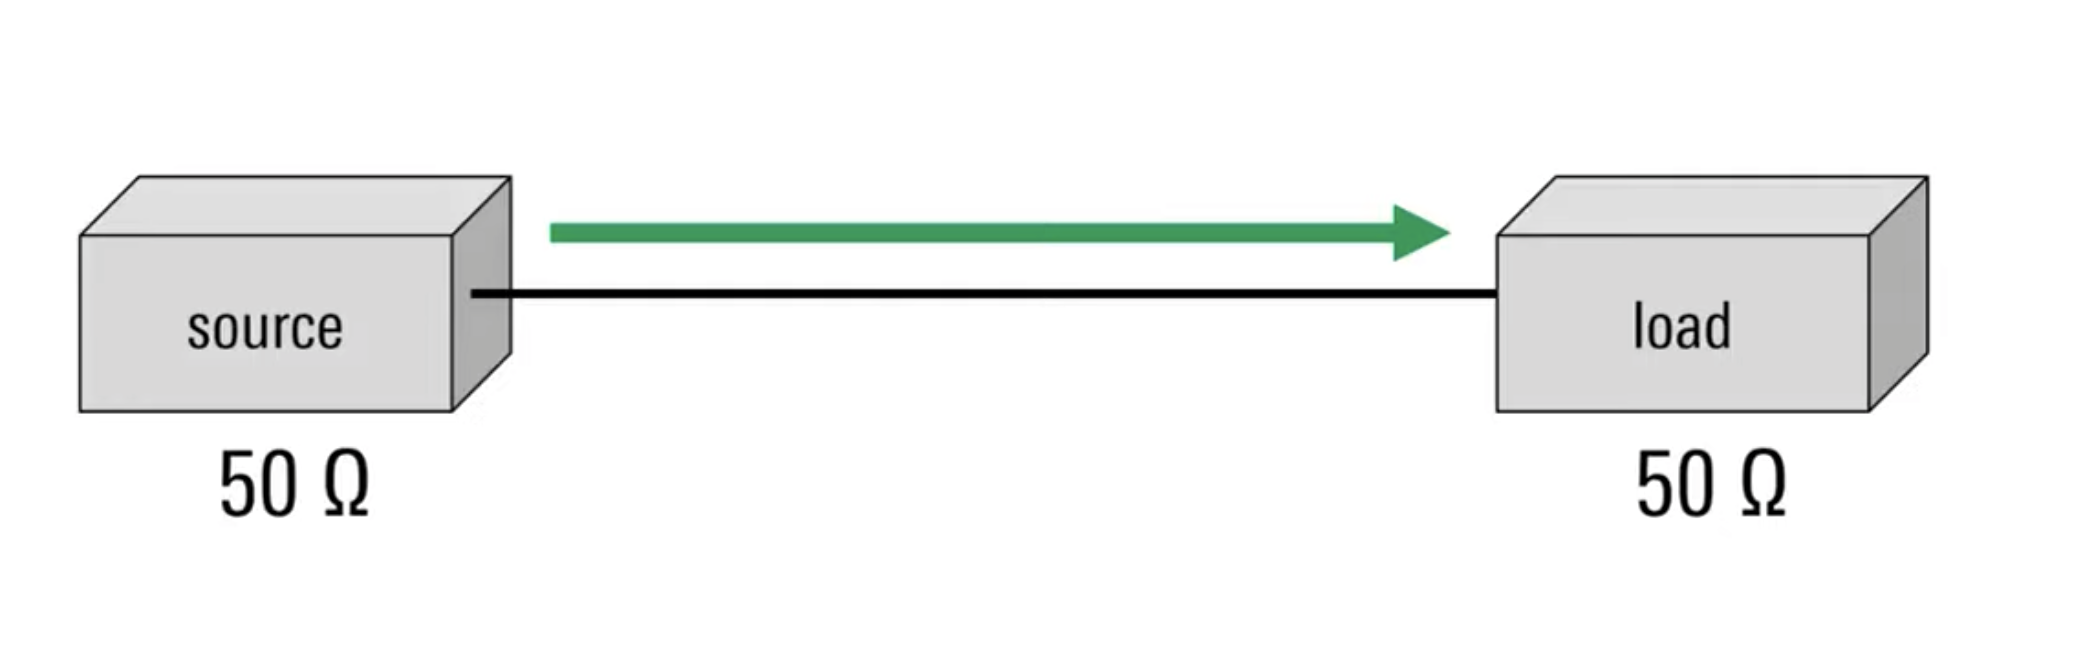
\includegraphics[width=0.75\linewidth]{images/impedance.png}
\caption{\label{fig:impedance}Узгоджений хвильовий опір.}
\end{figure}

\textbf{Важливо!} Опір антени — це величина, яка залежить від частоти.

\subsection{Зворотні втрати антени}

\textbf{Зворотні втрати} антени (англ. \textit{Return Loss}) --- це параметр, який описує, наскільки добре хвильовий опір антени узгоджений з хвильовим опором передавального або приймального тракту (кабеля). Це міра відбитої енергії від антени назад до джерела сигналу через невідповідність імпедансу між антеною і кабелем.

\begin{itemize}[noitemsep, topsep=8pt]
\item \textbf{Зворотні втрати} вимірюються в децибелах (дБ) і позначають різницю потужності, яка подається на антену, і яка відбилася від антени.
\item Високі значення зворотних втрат свідчать про те, що більша частина енергії передається через антену і лише незначна частина відбивається назад. Це є бажаним для оптимальної роботи системи.
\item Низькі значення зворотних втрат означають, що значна частина енергії відбивається назад до джерела сигналу, що свідчить про погане узгодження імпедансів і може призводити до втрат сигналу та зниження ефективності роботи антени.
\end{itemize}

\begin{figure}[H]
\centering
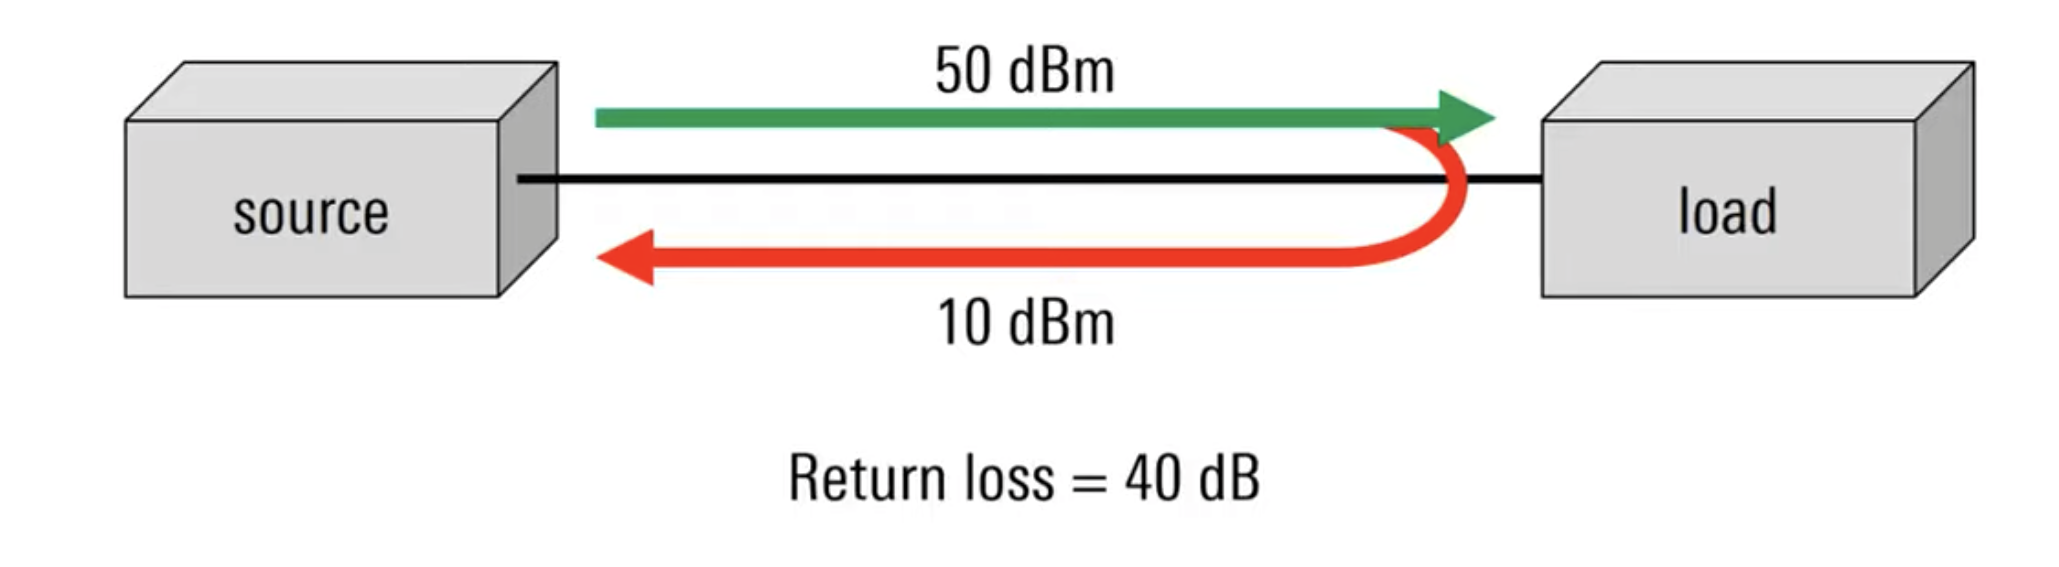
\includegraphics[width=0.75\linewidth]{images/return-loss.png}
\caption{\label{fig:return-loss}Зворотні втрати антени.}
\end{figure}

\subsection{КСХ антени}
\textbf{КСХ} (коефіцієнт стоячої хвилі, VSWR, SWR) антени — це параметр, який показує, наскільки добре антена узгоджена з хвильовим опором фідера (кабеля), до якого вона підключена. КСХ (англійською VSWR — Voltage Standing Wave Ratio) вказує на відносний рівень стоячих хвиль, що утворюються через невідповідність імпедансів антени і кабеля.

\begin{figure}[H]
\centering
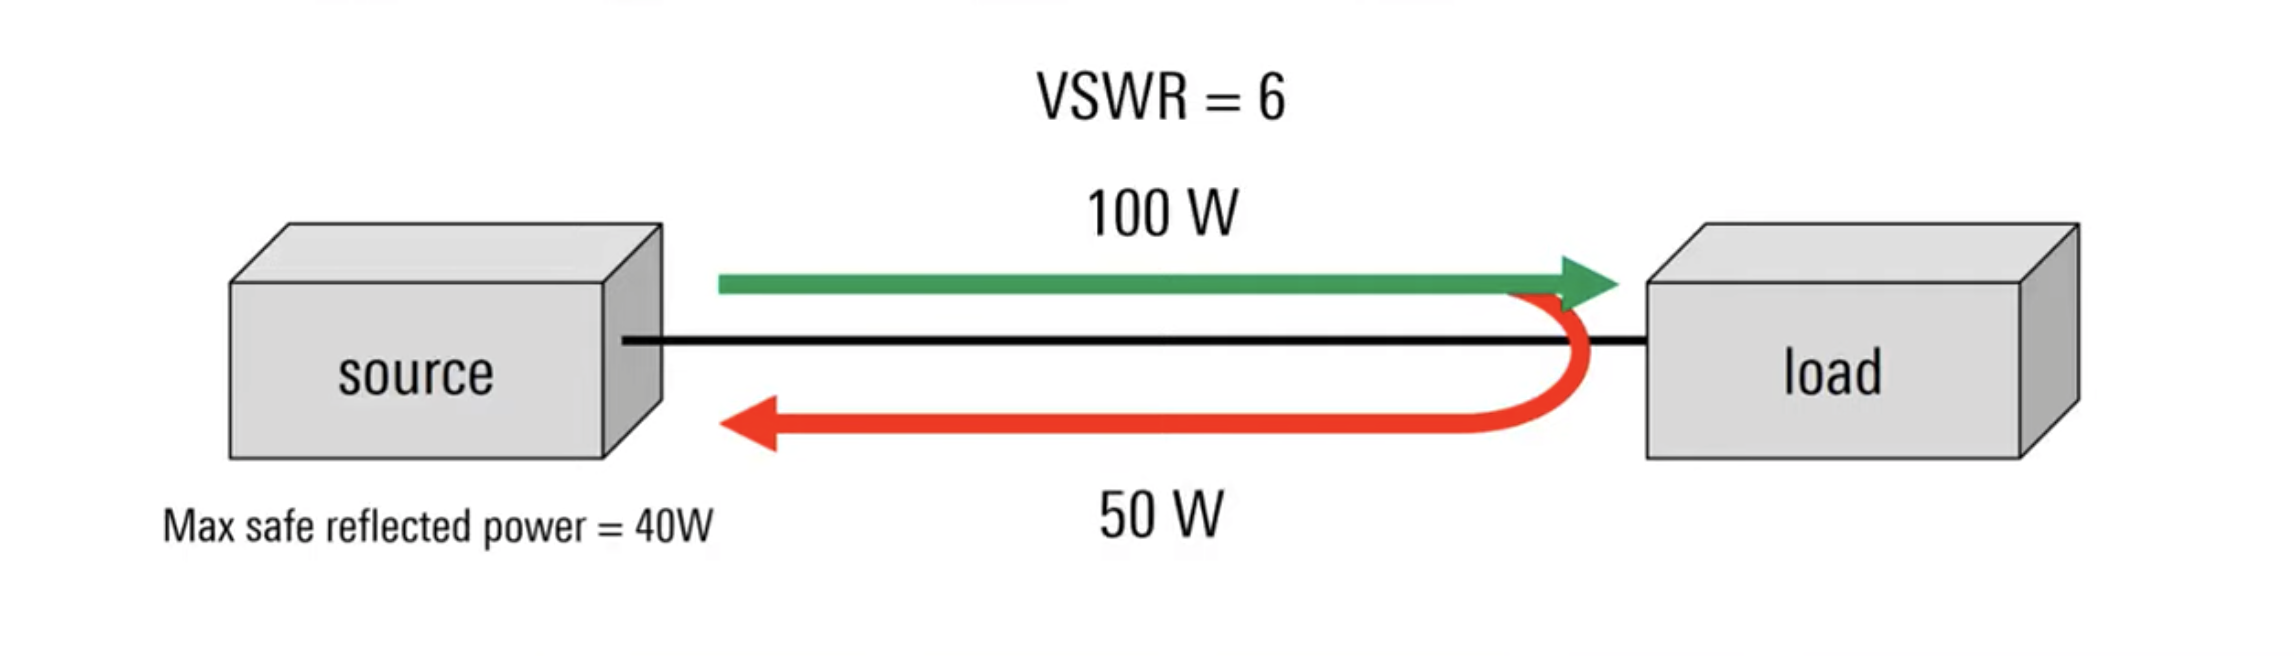
\includegraphics[width=0.75\linewidth]{images/swr.png}
\caption{\label{fig:swr}КСХ антени.}
\end{figure}

Високий КСХ вказує на те, що значна частина потужності сигналу не випромінюється антеною, а відбивається назад у фідер, що може призводити до різних проблем, таких як перегрів передавача, зниження ефективності передачі сигналу і навіть пошкодження обладнання.

\begin{table}[H]
\centering

\begin{tabular}{rcc}
\toprule
\textbf{SWR} & \textbf{\makecell{Voltage \\ reflected (\%)}} & \textbf{\makecell{Power \\ reflected (\%)}} \\
\midrule
1.0:1  & 0   & 0   \\
1.1:1  & 5   & 0.2 \\
1.2:1  & 9   & 0.8 \\
1.3:1  & 13  & 1.7 \\
1.4:1  & 17  & 2.8 \\
1.5:1  & 20  & 4   \\
1.6:1  & 23  & 5.3 \\
1.7:1  & 26  & 6.7 \\
1.8:1  & 29  & 8.2 \\
1.9:1  & 31  & 9.6 \\
\textbf{2.0:1}  & \textbf{33}  & \textbf{11}  \\
2.5:1  & 43  & 18.4 \\
3.0:1  & 50  & 25  \\
4.0:1  & 56  & 36  \\
5.0:1  & 67  & 44.4 \\
10.0:1 & 82  & 67  \\
\bottomrule
\end{tabular}
\caption{Відсоток відбиття напруги і потужності при певних значеннях КСХ.}
\end{table}

\begin{itemize}[noitemsep, topsep=8pt]
\item \textbf{Ідеальне значення КСХ}: Ідеальне значення КСХ --- це 1:1, що означає повне узгодження імпедансів антени і кабеля, при якому всі передані хвилі проходять через антену, і жодна енергія не відбивається назад до передавача.
\item \textbf{Підвищений КСХ}: Якщо КСХ більше 1:1, це означає, що існує певна невідповідність імпедансів, і частина енергії відбивається назад. Наприклад, КСХ 2:1 означає, що 10\% потужності сигналу відбивається, а 90\% передається антеною.
\item \textbf{Значення КСХ}: Зазвичай вважається, що КСХ до 1.5:1 є прийнятним для більшості систем. Вищі значення свідчать про погане узгодження, що може призводити до зменшення ефективності системи і підвищення ризику пошкодження передавача через відбиту потужність.
\end{itemize}


\subsection{Векторий аналіз}

При вимірі характеристик активних і пасивних радіопристроїв (антен, підсилювачів та ін.), а також властивостей різних матеріалів (поглинання та відображення радіохвиль, діелектрична постійна та ін.) широко використовуються векторні аналізатори електричних кіл.

Векторний аналізатор електричних ланцюгів — це прилад, який вимірює характеристики проходження сигналу через пристрій, що тестується, і характеристики відображення сигналу від його портів. Ці характеристики називаються S-параметрами.

Кожен S-параметр містить амплітудно-частотну (АЧХ) і фазо-частотну (ФЧХ) характеристики пристрою, що тестується у відповідному напрямку. Існує багато стандартних способів відображення виміряних S-параметрів на екрані векторного аналізатора електричних кіл. Ви самі можете вибирати, в якому вигляді переглядати результати: у вигляді графіка КСВ або зворотних втрат від частоти, діаграми Сміта, амплітуди, фази, загасання або посилення, групової затримки та ін.


Для того, щоб виконати вимірювання, аналізатор електричних кіл подає на тестований пристрій синусоїдальний сигнал і вимірює сигнал, який відбився, і сигнал, який пройшов через пристрій. Обидва сигнали (відбитий і минулий) відрізнятимуться за амплітудою та фазою від тестового синусоїдального сигналу. Якщо аналізатор електричних кіл може вимірювати лише амплітуду, він \textbf{називається скалярним}. Якщо аналізатор може вимірювати амплітуду і фазу, то він \textbf{називається векторним}. Практично всі сучасні аналізатори електричних кіл є векторними, тому що саме векторний аналізатор дозволяє найбільш повно виміряти характеристики пристрою, що тестується в заданому діапазоні частот.

\begin{figure}[H]
\centering
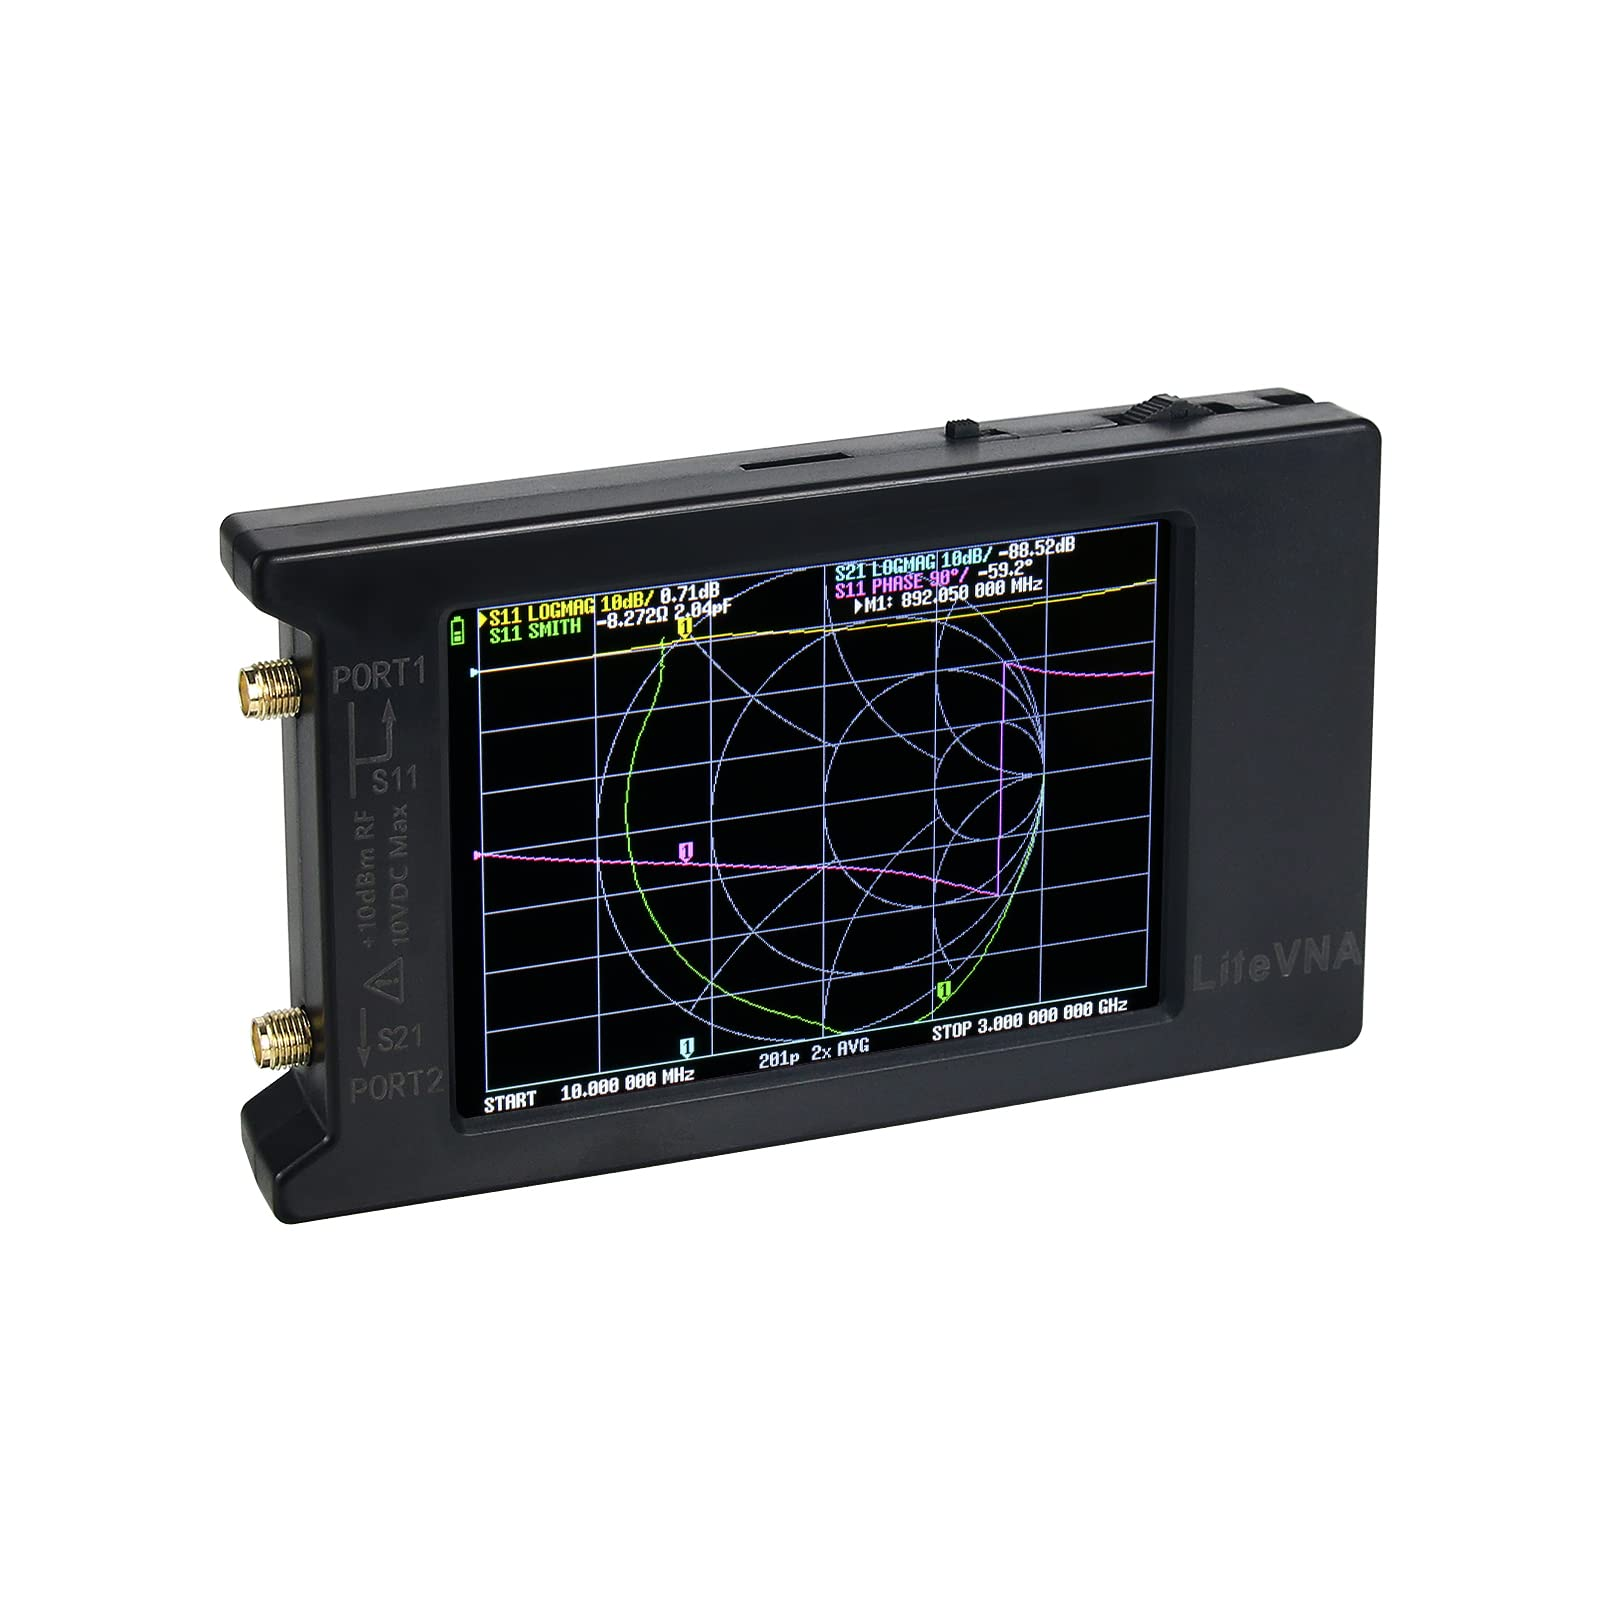
\includegraphics[width=0.6\linewidth]{images/lite-vna.jpg}
\caption{\label{fig:lite-vna}Векторний аналізатор LiteVNA-64.}
\end{figure}

В рамках нашого курсу векторний аналізатор нам цікавий як інструмент, який може вимірювати параметри антен, такі як КСХ (VSWR). Це потрібно для того, щоб якісно оцінити антену і визначити:

\begin{itemize}[noitemsep, topsep=8pt]
\item Чи справна антена.
\item Чи відповідає антена необхідним параметрам.
\end{itemize}

Практичний відеоматеріал стосовно застосування векторного аналізатора та вимірювання різних параметрів, таких як КСХ антени та затухання у кабелі, \href{https://www.youtube.com/watch?v=S4V4TL_5KQg}{доступний за посиланням}.

\subsection{Додаткові матеріали по темі}
\begin{itemize}[noitemsep, topsep=8pt]
\item \href{https://sprotyvg7.com.ua/wp-content/uploads/2023/05/Osnovni-harakterystyky-anten_ukr.pdf}{Основні характеристики і типи польових антен.}
\item \href{https://www.tehencom.com/Categories/Network_Analyzers/Basics/Network_Analyzers_Basics-u.htm}{Що таке векторний аналізатор електричних ланцюгів}.
\item \href{https://www.youtube.com/watch?v=1me_Tz3CFmk}{2 Антенки FPV: діаграма спрямованості і підсилення (gain) в dBi}
\end{itemize}

\section{Пошук джерела радіовипромінювання}
 
\subsection{Вимірювання напруженості поля}
 
Одним із найпростіших і найефективніших способів знайти передавач є використання вимірювача напруженості поля з регульованим атенюатором\footnote{В другій частині цього навчального матеріалу у розділі \ref{sec:radio:metter}  наведена схема саморобного вимірювача напруженності поля}. 
 
\begin{figure}[H]
 	\centering
 	{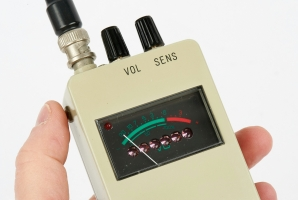
\includegraphics[width=0.6\linewidth]{images/rdf-small.jpg}}
 	\caption{\label{fig:rds:small}Портативний пристрій для вимірювання напруженності поля.}
\end{figure}
 
Вимірювання напруженості поля широко використовується й сьогодні, часто в поєднанні з іншими методами радіопеленгації, такими як триангуляція та автоматичне визначення напрямку, особливо на завершальному етапі для виявлення точного місцезнаходження, з якого працює передавач.

 
\subsection{Пеленгатори та пеленгаційні системи} 
\textbf{Пеленгатор} --- це пристрій або система, яка визначає напрямок (азимут, він же пеленг) на джерело радіовипромінювання. Його основне завдання -- виявити кутове положення джерела відносно пеленгатора. Пеленг визначається в градусах відносно півночі за годинниковою стрілкою, тобто напрямок на північ -- це 0° або 360°, на схід -- 90°, на південь -- 180°, а на захід -- 270°. 

Ми пам'ятаємо, що є три фізичні властивості радіохвиль, що потенційно можуть змінюватися під час поширення у просторі, а саме амплітуда, частота та фаза, але окрім цього у нас супутні явища, які негативно впливають на визначенню пеленгу, такі як перевідбиття, розсіювання та заломлення хвиль. У визначені азимутів та наявності сигналу, який, може, надходить з кількох місць або змінює рівень через конструктивні або деструктивні перешкоди, є значною проблемою, і тому багатопроменевість, або те що називають ще multipath, зазвичай є найбільшою проблемою в пеленгації. У багатьох випадках якісна та гарна система або методологія пеленгування залежить, перш за все, від її здатності отримувати якісні результати пеленгування навіть за наявності  багатопроменевості. 

Пеленгаційні системи можуть давати похибку кута в межах від Х до Y градусів, її ще можуть називати кутом розкриття комплексу. Зазвичай, ця інформація зазначається виробником в ТТХ і дуже залежить від методу, який використовується для пеленгування,  конструктивних особливостей пеленгаційного комплексу, а саме геометрії розташування антен по відношенню одна до одної, їх типу та багатьох інших чинників. Головне, що варто знати, це те, що кут похибки має лінійну природу, тобто, чим більше відстань від пеленгатора, тим буде більше зона невизначенності джерела радіовипромінювання.

\begin{figure}[H]
	\centering
	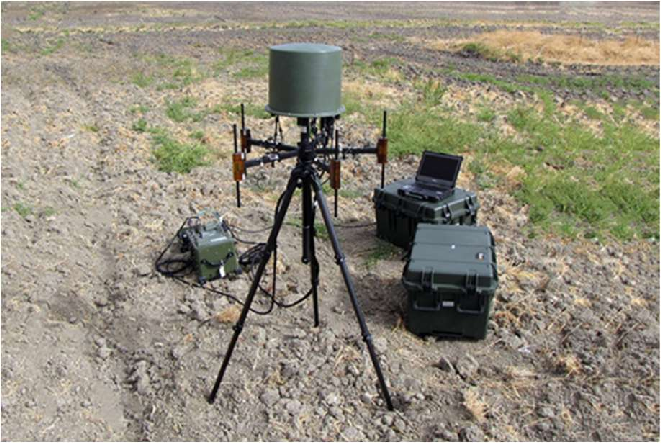
\includegraphics[width=0.8\linewidth]{images/tsi.png}
	\caption{\label{fig:tsi} Стаціонарний пеленгатор TСI 903S на щоглі}
\end{figure}

 
Визначення пеленгу не дає нам інформації про точне розташування джерела радіовипромінювання, а дає лише нарямок, тому ми поступово наближаємось до терміну триангуляції.  

\subsubsection{Триангуляція та зведення пеленгів}
\textbf{Триангуляція} --- це метод визначення місцезнаходження об'єкта, що використовується в навігації та радіопеленгуванні. Принцип полягає в тому, що розташування об'єкта обчислюється за допомогою двух (максимум трьох) пеленгаційних систем за рахунок визначення азимутів до джерела радіовипромінювання. Збільшення кількості пеленгів, що використовуються в розрахунку тріангуляції, зазвичай не забезпечує додаткової точності. Перетин цих азимутів по конкретній радіо частоті утворює зону, яка має назву еліпс невизначеності, яка по суті і буде визначати фактичне розташування емітера. Джерело радіовипромінювання буде знаходитись саме в межах утворенної фігури і не завжди є її центром. 

\begin{figure}[H]
	\centering
	{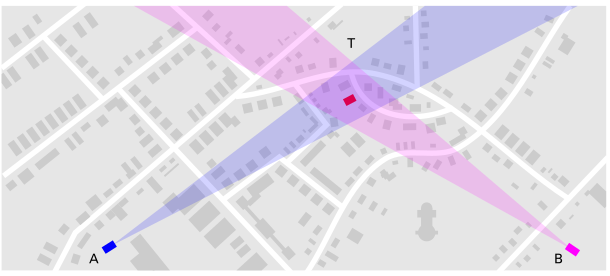
\includegraphics[width=0.6\linewidth]{images/df_triangulation.png}}
	\caption{\label{fig:triangulation}Зведення пеленгів.}
\end{figure}

Еліпс невизначенності за своєю формою може бути різним і залежить від того, який кут утворюється в місті перетину цих пеленгів. Бажаний кут перетину, який буде давати мінімальну похибку, повинен бути 90 градусів, тоді два пеленги утворюють коло в центрі, відповідно самий небажаний варіант, це такий перетин, що утворює гострий кут. Для госторого кута еліпс невизначенності стає значно більшим.

\begin{figure}[H]
	\centering
	{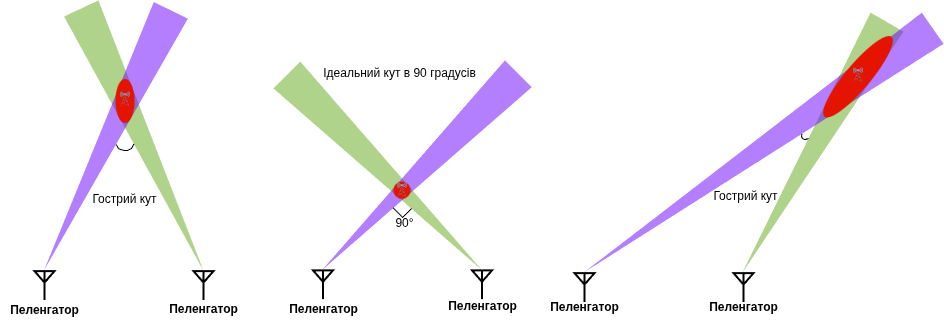
\includegraphics[width=0.8\linewidth]{images/triangulation.png}}
	\caption{\label{fig:triangulations} Триангуляція та еліпси невизначеності.}
\end{figure}

Триангуляція може бути виконана і одним пеленгатором, зазвичай цей процес виконується по статичним цілям і у більшості випадків, це ті що будуть розташовані на землі. Принцип зведення триангуляції в цьому випадку доволі простий, виконується зміна позиції пеленгатора на різні локації та фіксація азимутів по частоті, що представляє для нас інтерес. Термін зміни локації визначається ургентністю локалізації джерела радіовипромінювання. Зафіксовані азимути з різних координат будуть утворювати перетин, що і буде визначати зону джерела радіовипромінювання. 

\begin{figure}[H]
	\centering
	{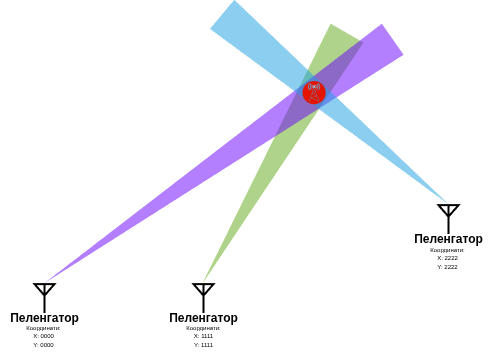
\includegraphics[width=0.5\linewidth]{images/one_device_triangulation.png}}
	\caption{\label{fig:triangulations} Триангуляція одним пеленгаторомз та зміна позиції.}
\end{figure}

\begin{figure}[H]
	\centering
	{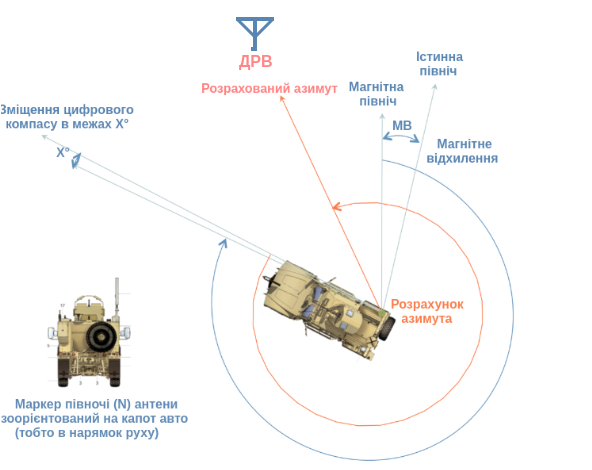
\includegraphics[width=0.6\linewidth]{images/mobile_df.png}}
	\caption{\label{fig:triangulations} Мобільний рухомий пеленгатор.}
\end{figure}


На поточний момент існують пеленгаційні системи, який дозволяють визначати та створювати засічки на рухомих платформах, тобто, це може бути безпілотний літальний апарат або комплекс на колесній базі.
Рухаючись вздвовж зони інтересу, система в автоматичному режимі може визначати напрямок випромінювання та збирати інформацію по пеленгам в радіочастотному діапазону, що представляє для нас інтерес. Мобільні платформи в такому форматі зазвичай використовують курсовий компас на базі GPS, додатково ще може використовуватись магнітний компас для визначення напрямку магнітного напрямку на північ. Це дозволяє робити розрахунок фактичного азимута до джерела радіовипромінювання. 

\begin{figure}[H]
	\centering
	{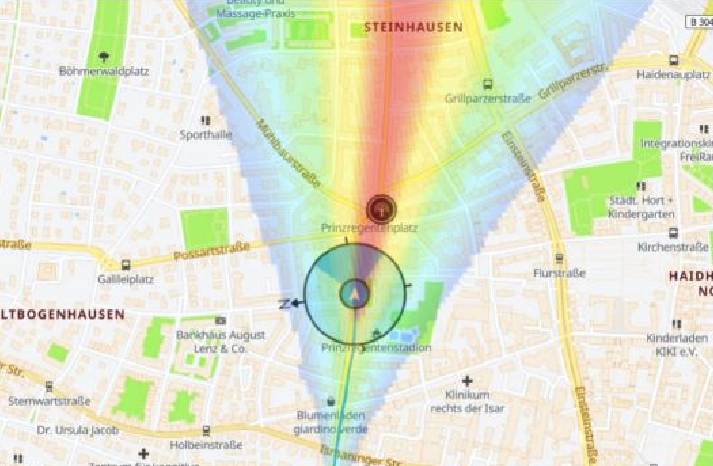
\includegraphics[width=0.6\linewidth]{images/heatmap-df.png}}
	\caption{\label{fig:triangulations} Побудова теплової карти та створення засічок мобільним засобом.}
\end{figure}

В деяких комплексах використовується концепція майстер-слейв для зведення триангуляцій, тобто є керуюча станція і підлеглі. Вся робота виконується в цьому випадку на майстер станції і зведення пеленгів відбувається в автоматичному режимі саме на цій станції. На комплексах, що зав'язуються між собою у групи супер важливо робити синхронізацію по часу. Синхронізація по часу потрібна для того, що б зводились пеленги між станціями, у випадку розбіжності по часу зведення пеленгів відбуватись не буде. Синхронізація по часу може бути виконана через мережу інтернет, а саме системний час з вашого комп'ютера та станцією, або ж з використанням окремого NTP серверу. Виконувати синхронізацію через GPS не рекомендовано біля лінії бойового зіткнення і сурово заборонено залишати її завжди ввімкненою.


\subsection{Методи пеленгування}
 
\subsubsection{Ручне пеленгування}
Основна форма справжнього пеленгування полягає у використанні (більш-менш) напрямленої антени, такої як диполь, відкрита петля, віконна, Адкока, Ягі або логоперіодична антена. Підключивши антену до приймача і повертаючи її, можна визначити кут максимального або мінімального рівня сигналу.

У випадку портативного приймача та антени перехоплювач може орієнтувати антену в напрямку передавача, поки його не знайде найпотужніший сигнал. Хорошим прикладом сучасної ручної пеленгаційної системи є приймач Rohde \& Schwarz PR-100 у поєднанні з портативною антеною HE-300. 

\begin{figure}[H]
\centering
{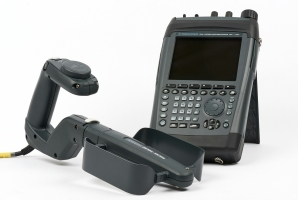
\includegraphics[width=0.6\linewidth]{images/rds-rs-100.jpg}}
\caption{\label{fig:rds:pr100}Портативний пристрій Rohde \& Schwarz PR-100.}
\end{figure}

Найбільшою перевагою ручного визначення пеленгу є його низька вартість та портативність, особливо при використанні ручних антен та портативних приймачів. Навіть при використанні штатива або іншого монтажного пристрою, ручні системи майже завжди є компактними та можуть бути швидко розгорнуті практично в будь-якому місці з мінімальним часом налаштування. Підходи на основі ручного визначення пеленгу часто можуть давати прийнятні результати. Проте, існує ряд обмежень, коли йдеться про ручний підхід до пеленгації. Ефективність цієї методології може сильно залежати від рівня кваліфікації та досвіду оператора, оскільки антена зазвичай повертається вручну, а визначення пеленга здійснюється оператором-людиною. Точність може бути низькою для віддалених цілей також через людський фактор – навіть зі штативом та дуже вузькою діаграмою спрямованості антени, величина похибки пеленга, внесеної людиною, може призвести до суттєвих похибок визначення місцезнаходження на відстанях понад кілька сотень метрів. Ручні методи визначення кута не працюють добре при спробі знайти короткочасні сигнали. Сигнал, який з'являється лише на кілька секунд, може «з'явитися і зникнути», перш ніж оператор встигне повернути антену та визначити та зафіксувати пеленг. Ці обмеження є однією із причин розробки методів автоматичного пеленгування.

\subsubsection{Доплерівське пеленгування}
У системі пеленгування, що базується на ефекті Доплера, антену можна уявити як таку, що обертається з постійною швидкістю в горизонтальній площині, як показано на малюнку нижче. Круговий рух антени \textit{A} викликає частотну модуляцію синусоїдальної форми \textit{fm} у прийнятому сигналі \textit{fc}. Цей ефект відомий як доплерівський зсув частоти. Фаза $\phi$ синусоїдальної модуляції \textit{fm} буде визначатися кутом падіння $\alpha$ прийнятого сигналу \textit{fc}. Порівнюючи фазу джерела керування двигуном та демодульованого сигналу, можна визначити початковий кут падіння прийнятого сигналу.

\begin{figure}[H]
\centering
{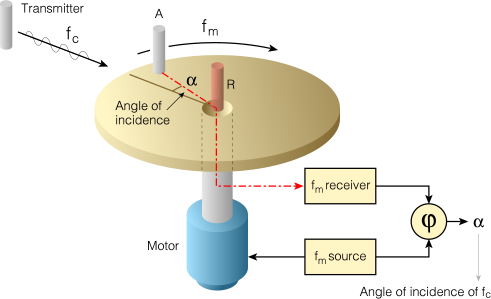
\includegraphics[width=0.6\linewidth]{images/rdf-dopler.png}}
\caption{\label{fig:rdf:dopler}Cхематичне зображення принципу вимірювання напрямку джерела випромінювання використовуючи ефект Доплера.}
\end{figure}

На практиці обертання антени імітується електронним комутуванням (перемиканням) між кількома дискретними антенами, рівномірно розташованими по колу. Зазвичай, більшість систем складається з чотирьох або восьми дискретних антен. Крім того, референсна антена \textit{R} часто розташовується в центрі кола для прийому у звичайному режимі. У цьому випадку референсний сигнал використовується для усунення частотної модуляції, викликаної голосом, щоб фаза частотної модуляції, викликаної ефектом Доплера \textit{fm}, могла бути визначена більш точно.

Доплерівський пеленгатор є відносно недорогим порівняно з іншими автоматичними методологіями пеленгатора. Частково причина низької вартості доплерівського пеленгатора полягає в тому, що він не є конструктивно складним. Майже всі доплерівські системи розроблені для роботи на частотах VHF або (низьких) UHF частотах. Існує ряд обмежень, властивих доплерівському пеленгатору. По-перше, доплерівські системи пеленгатора більш-менш вимагають, щоб цільовий сигнал був постійним, безперервним або подібним. Доплерівський метод не добре працює для локалізації переривчастих та непостійних сигналах, або дуже широкосмугових або шумоподібних сигналів. Оскільки доплерівські антенні решітки складаються з вертикальних елементів, ці решітки погано працюють під час спроби локалізувати горизонтально поляризовані сигнали – втрати через межі крос-поляризації можуть легко становити від 20 до 30 дБ. Автоматичні системи радіопеленгації на основі доплерівського ефекту є чимось на зразок «початкової» системи радіопеленгації, яка може бути гарним вибором для певних застосувань, особливо коли вартість є важливим фактором.

\subsubsection{Watson Watt}
Ватсон-Ватт — це система, яка побудована на порівнянні амплітуд. Це одна із самих старих методологій пеленгації, розроблена невдовзі після Першої світової війни, і названа на честь її винахідника, Роберта Александра Ватсона-Ватта. Методологія пеленгації Ватсона-Ватта базується на властивостях спеціального типу антени, яку зазвичай називають антеною Адкока. Аантена Адкока складається з чотирьох вертикальних елементів, розташованих попарно, розташованих на однаково-рівній відстані один від одного. Це створює діаграму спрямованості антени, що складається з двох пелюсток у формі вісімки. Кожна з двох діаграм спрямованості у формі вісімки має максимальну чутливість вздовж осі, що проходить через обидві антени та нулі, перпендикулярні цій осі. Таке розташування дає унікальний набір величин для кожного напрямку вхідного сигналу.


\begin{figure}[H]
	\centering
	{\includegraphics[width=0.2\linewidth]{images/adkock_antenna.jpeg}}
	\caption{\label{fig:rdf:dopler} Діаграма спрямованості антени Адкока.}
\end{figure}

На схемі зоображені дві різні пари різними кольорами, які розташовані ортогонально одна відносно одної. Сигнал, що буде проходити зверху до низу або знизу до верху, тобто по зеленій осі, буде мати максимальну чутливість і мінімальну по відношенню до синьої осі. Сигнал, що буде приходити під кутом в 45 градусів по відношенню до зеленої та синьої осі може приводити до однакових результатів на обох парах антен. Відповідно, будь-який довільний напрямок можна визначити, порівнюючи амплітуди на двох осях.

\begin{figure}[H]
	\centering
	{\includegraphics[width=0.7
		\linewidth]{images/adkock_antennas.png}}
	\caption{\label{fig:rdf:dopler} Варіації антен для метода Ватсон-Ватта.}
\end{figure}

Найчастіше, окремі елементи антени реалізуються як монополі, коли є площина заземлення, з якою потрібно працювати, або як диполі в системах, що встановлюються на стовпах або вежах. Такий самий тип діаграми спрямованості та поведінки можна отримати також за допомогою пари схрещених петель. Що стосується розташування елементів, найбільше питання полягає в тому, наскільки далеко один від одного розташовувати елементи. Ця відстань є компромісом між точністю та чутливістю – розміщення елементів ближче один до одного дає вищу точність, але чутливість краща, коли елементи розташовані далі один від одного.

Як і всі інші методи пеленгування, метод Watson-Watt має свій власний набір переваг, недоліків та практичних міркувань. Одна з переваг методу Watson-Watt серед інших методів пеленгування полягає в тому, що він добре підходить для HF діапазону, головним чином завдяки легкості, з якою менші антени можуть бути реалізовані на цих частотах. Метод Watson-Watt також дуже швидкий. Отримання фактичного пеленгу не потрібує важких обчислень, оскільки система просто порівнює амплітуду на двох різних парах антен. Watson-Watt має хорошу точність і чутливість. Основним недоліком методу Watson-Watt є те, що він не може вимірювати кут висоти для ДРВ і якщо ціль значно вище або нижче площини антени, точність може страждати.

\subsubsection{Принцип Homer}
Принцип Homer\footnote{Також можна зустріти цей метод під назвою \textit{Монопульс на основі порівняння амплітуд}.} складається з двох спрямованих антен, які направлені трохи вбік від центру. Використовуючи діаграми спрямованості антен і швидко перемикаючись між ними, можна виміряти стрибки сили сигналу, за винятком випадку, коли передавач знаходиться прямо попереду, в такому разі сила сигналу на обох антенах буде однаковою (точка P мал. \ref{fig:homer}).

\begin{figure}[H]
\centering
{\includegraphics[width=0.3\linewidth]{images/homer.png}}
\caption{\label{fig:homer}Cхематичне розташування антен.}
\end{figure}

Діаграма вище показує, як це працює. Дві антени \texttt{A} і \texttt{B} мають однакові діаграми спрямованості, але вони спрямовані трохи в різні боки, наприклад, на \texttt{$+15^\circ$°} і \texttt{$-15^\circ$} у напрямку джерела випромінювання. Коли передавач знаходиться прямо попереду, сигнал від обох антен буде однаковим \texttt{A=B}, і різниці у силі сигналу не буде. Це показано в точці P на діаграмі вище.

\begin{figure}[H]
\centering
{\includegraphics[width=0.7\linewidth]{images/homer_meter.png}}
\caption{\label{fig:homer:meter}Функціональна схема методу Гомера.}
\end{figure}

Коли сила сигналу між двома антенами різна (наприклад, коли \texttt{B>A}), то рівні сигналів від антен будуть також різними і ця різниця є мірою для визначення кута надходження сигналу. Точка \texttt{Q} у прикладі. Діаграма вище показує, як сила сигналу з обох антен впливає на вихідні показники. У стані спокою \texttt{A=B} стрілка індикатора вказує вгору \texttt{0V}.

\begin{figure}[H]
\centering
{\includegraphics[width=0.6\linewidth]{images/isolog-3d-160.png}}
\caption{\label{fig:isolog-3d}Масив антен встановлених на єдиному шасі. Антена IsoLOG 3D 160 від \href{https://aaronia.com/en/produkte/antennas/isolog-3d-df}{Aaronia}.}
\end{figure}

На базі цього рішення можна побудувати антену яка здатна визначати не тільки напрямок об'єкту по горизонталі(азимут відносно півночі), а також кут по вертикалі. На мал. \ref{fig:isolog-3d} зображено масив із антен поєднаних у єдину систему. Комплекс із застосуванням таких антен може обчислювати місцезнаходження (по зведеному пелелегу) і висоту джерела сигналу. 

\subsubsection{Кореляційний інтерферометр}

Кореляційний інтерферометр визначає пеленги шляхом обчислення різниці у фазі прийнятих сигналів, що спостерігається на кількох спільно розташованих антенних елементах. Антени кореляційного інтерферометру зазвичай використовують непарну кількість антенних елементів, розташованих по колу. 

\begin{figure}[H]
	\centering
	{\includegraphics[width=0.5\linewidth]{images/df_int_wave.png}}
	\caption{Cхематичне зображення послідовності надходження сигнала на антени інтерферометра.}
\end{figure}

Щоб пояснити принципи кореляційної інтерферометра, ми розглянемо приклад п'ятиелементної антени. П'ять антен розміщені по колу, причому одна з антен, є  (головною) референсною антеною, вона під номер 1. Коли сигнал надходить на антену під заданим кутом, наприклад, 45 градусів, виміряний сигнал буде зміщений по фазі на кожному з п'яти елементів антени. Процес калібрування виконується для кожного кута, від 0 до 360 градусів, з кроком в один градус. Результатом є таблиця, яка містить фазові зміщення для всіх кутів вхідного сигналу. Вимірювання фазових різниць - це частина назви цієї методології, що означає «інтерферометрія».

\begin{figure}[H]
	\centering
	{\includegraphics[width=0.6\linewidth]{images/correletion_interf.png}}
	\caption{Вимірювання фазового здвигу для інтерферометра.}
\end{figure}

Коли цільовий сигнал надходить на антенну, прийняті фазові зміщення вимірюються на кожній антені. Кореляція між виміряними фазовими зміщеннями та каліброваними або ідеальними фазовими зміщеннями розраховується для кожного кута приходу. Цей процес повинен дати чіткий пік кореляції, з якого можна визначити пеленг або кут приходу.


\begin{figure}[H]
	\centering
	{\includegraphics[width=0.7\linewidth]{images/correletaion_interft_meas.png}}
	\caption{Визначення пеленгів з кореляції зі значеннями рефернсної фази.}
\end{figure}

Окрім отримання результату пеленгу, кореляційна інтерферометрія також забезпечує якість пеленгу. Обидва ці графіки кореляції дають пік, який відповідає пеленгу 127 градусів. Однак графік ліворуч показує набагато сильнішу кореляцію під цим кутом, ніж графік праворуч. Тож, хоча обидва набори результатів дають однаковий пеленг, ми матимемо вищий ступінь впевненості в одному з результатів, ніж в іншому. Цей тип результату «якості пеленгу» є унікальним для кореляційної інтерферометрії.

\begin{figure}[H]
	\centering
	{\includegraphics[width=0.7\linewidth]{images/correletaion_interfer_graphs.png}}
	\caption{Якість характеристики пеленгу.}
\end{figure}

Антени кореляційного інтеферометру також можуть бути реалізовані в дуже малих корпусах з хорошою точністю, але стійкість її до таких речей, як відбиття та багатопроменеве поширення, збільшується зі збільшенням діаметра антени. Відбиття та багатопроменеве поширення викликають зміни фази прийнятого сигналу. Збільшення апертури (діаметр, поділений на довжину хвилі) антени типу кореляційного інтерферометра до значення більше одиниці покращує точність, оскільки вплив цих "вигнутих" ізофазних ліній зменшується. Однак, порівняно з іншими методологіями пеленгування, що обговорювалися попередньо, кореляційний інтерферометр ставить досить суворі вимоги до антени з точки зору проектування та виробничого допуску. Можна в кустарних умовах зробити антени для ручного пеленгування, доплерівського та Ватсон-Ваттового методів та отримати досить прийнятні результати, але антени типу кореляційного інтерферометра вимагають дуже спеціалізованих інженерних та виробничих ресурсів через високі вимоги до проектування та виробничих допусків. Відповідно кореляційний інтерферометр має кілька суттєвих переваг порівняно з іншими методологіями пеленгації. Перша — це дуже висока точність, зазвичай один градус або менше в ідеальному середовищі. Жодна інша методологія пеленгації не може забезпечити пеленгації з подібним рівнем точності. Оскільки кореляційний інтерферометр порівнює різниці фаз на кількох елементах одночасно, вона пропонує дуже високу стійкість до багатопроменевості порівняно з іншими методологіями. Поляризація сигналу не впливає на точність, це є один з головних недоліків доплерівської методології і системи гарно працює з урахуванням висот, яка актуальна для пеленгації методом Ватсона-Ватта. 

% https://www.cryptomuseum.com/df/df.htm

\subsubsection{TDOA - Time differenc of arrival}
Методологія TDOA базується на часі, що в кінцевому випадку визначає місцезнаходження випромінювача на основі часу отримання сигналу в кількох місцях. Основний принцип різниці часу полягає в наступному: три або більше приймачів розміщуються в різних місцях, і всі ці приймачі отримують сигнал. У більшості випадків відстані між передавачем і кожним приймачем різні, тому час, коли сигнал надходить до кожного приймача, також буде різним. Ми можемо представити цю різницю часу як криві або гіперболи, і місцезнаходження передавача буде на перетині цих гіпербол. Фактично, різниця часу приходу іноді також називається "гіперболічною" пеленгацією, оскільки ми визначаємо місцезнаходження передавача за допомогою цих гіпербол.

Для створення гіперболи потрібні два приймачі, і вимірюється різниця часу прийому на обох приймачах. Якщо різниця часу дорівнює нулю, то гіпербола буде прямою лінією між двома приймачами, оскільки кожна точка на цій лінії знаходиться на однаковій відстані від обох приймачів. З іншого боку, гіпербола буде криволінійною, якщо різниця в часі прибуття до двох приймачів не дорівнює нулю.

\begin{figure}[H]
	\centering
	{\includegraphics[width=0.7\linewidth]{images/tdoa.png}}
	\caption{Утворення гіперболи заснованій на різниці в часі.}
\end{figure}

Якщо є три приймачі, то буде три гіперболи – одна між приймачами 1 і 2, інша між приймачами 2 і 3, і третя між приймачами 1 і 3. Розташування випромінювача знаходиться
на перетині цих трьох кривих. Можна мати більше трьох станцій, але
потрібно щонайменше три станції для отримання однозначного визначення місцезнаходження.


\begin{figure}[H]
	\centering
	{\includegraphics[width=0.4\linewidth]{images/tdoa-3p.png}}
	\caption{Визначення позиції емітера за рахунок TDOA.}
\end{figure}

Система пеленгації на основі TDOA складається з мережі взаємопов'язаних датчиків та головної станції. Отримані сигнали, оцифровуються, тобто перетворюються на IQ-дані, а потім передаються на головну станцію. Основною вимогою для методики TDOA є супер точна синхронізація по часу. Станції між собою повинні бути синхронізовані і зазвичай це реалізується за рахунок GPS або ж атомного годиника. Оримавши IQ-данні з чітко виставленими мітками часу головна станція обчислює взаємну кореляцію, використовуючи дані з кожної станції, а результати цього розрахунку визначають різницю часу, які потім використовуються для побудови гіпербол.

Для визначення часу прибуття (TDOA) потрібна різниця в часі прибуття (дельта t), і ця різниця в часі визначається за допомогою кореляції. Визначається опорний час, і кореляція розраховується при різних часових зсувах. Результати кореляції дають корелограму, пікове значення якої відповідає часовому зсуву.


\begin{figure}[H]
	\centering
	{\includegraphics[width=0.6\linewidth]{images/tdoa_corelelogram.png}}
	\caption{Корелограма та визначення дельта t}
\end{figure}

Коли сигнал широкосмуговий, зазвичай неважко знайти чіткий пік кореляції для використання в TDOA. Однак, якщо сигнал вузькосмуговий, стає набагато важче знайти чіткий пік кореляції на корелограмі. Без чіткого піку, який би відображав різницю в часі прибуття, важко створити точну гіперболу. Важливо пам'ятати, що системи пеленгації на основі TDOA дають точніші результати при спробі знайти широкосмугові сигнали.

Всі попередні методи пеленгування, такі як доплерівський, Ватсон-Ватт або кореляційний інтерферометр, вимагали спеціальні антени. TDOA зосереджується на часі надходження сигналу, а не на напрямку чи куті, з якого цей сигнал надходить, і вимагає збору та позначення часу даних у кількох точках одночасно. Тому пеленгування на основі TDOA зазвичай реалізується у вигляді спеціально створених датчиків, які містять приймач та ненаправлену антену. Датчики оцифровують отримані радіочастотні сигнали у вигляді IQ даних та позначають час цих даних. Ці дані з позначками часу потім надсилаються до головної станції обробки даних через певний тип каналу передачі даних. Для гарної точності на більшій площі потрібна велика кількість таких датчиків, тому спеціалізовані датчики TDOA, як правило, є відносно недорогими та мають нижчу радіочастотну продуктивність, ніж приймачі, що використовуються в інших методах пеленгації.

Результати TDOA мають точність приблизно до кількох сотень метрів, що залежить як від методології та самих датчиків, так і від типу сигналу цілі, тобто широкосмуговий чи вузькосмуговий. Найкраща точність досягається, коли емітер більш-менш оточений датчиками, але поза цією зоною точність визначення місцезнаходження може бути низькою. Наприклад, якщо ціль має датчики з усіх боків, точність зазвичай буде хорошою. З іншого боку, якщо ціль знаходиться поза сенсорною мережею, результати
часто низькі. Тому часто потрібно мати певне уявлення про те, де знаходиться або
буде знаходитися ціль, перш ніж розгортати датчики. Це не є проблемою при спробі охопити певну зону, але обмежує корисність TDOA в спеціальних застосуваннях пеленгації. 


\begin{figure}[H]
	\centering
	{\includegraphics[width=0.6\linewidth]{images/tdoa_location_impact.png}}
	\caption{Вплив розташування сенсорів на позиціонування емітера}
\end{figure}

Додавання додаткових датчиків TDOA до мережі забезпечує кращу точність, але в певний момент (зазвичай близько шести датчиків) додаткового покращення немає, і час розрахунку різко зростає. TDOA також пропонує те, що називається «коефіцієнтом близькості», що означає, що система з більшою ймовірністю отримуватиме слабші сигнали, якщо в області є багато датчиків – ймовірність того, що один із датчиків буде фізично ближче до джерела, вища.

\subsection{Додаткові матеріали по темі}
\begin{itemize}[noitemsep, topsep=8pt]
	\item \href{https://cdn.rohde-schwarz.com/am/us/campaigns_2/a_d/Intro-to-direction-finding-methodologies~1.pdf}{An Introduction to Direction Finding}
	\item \href{https://www.cryptomuseum.com/df/df.htm}{Radio Direction Finding}	
	\item \href{http://www.homingin.com/newdopant.html}{Wide-Range Antenna Arrays For the Roanoke Doppler}
\end{itemize}


\newpage
\section{Вибір розташування пеленгаційної системи}
\label{sec:DF Placement}

Одним із критично важливих пунктів для ефективного пеленгування джерел радіовипромінювання є визначення гарної та ефективної точки розташування пеленгаційної антени. В першу чергу для вирішення цієї задачі треба визначитись з цілями та діапазонами частот, по яким буде працювати пеленгаційний компекс. Бо маючи  супер дорогий та ефективний комплекс, за асторономічні гроші, але не виставивши його з усіма вимогами екіпаж ризикує отримувати інформацію сумнівної якості.

\begin{figure}[H]
	\centering
	{\includegraphics[width=0.8\linewidth]{images/dominant_height.png}}
	\caption{\label{fig:triangulations} Вибір домінуючої висоти.}
\end{figure}

Отже, цілі для пеленгаційних систем можно умовно поділити на дві групи: наземні та повітряні. Робота по цим цілям буде відрізнятись, адже повітряні цілі, будуть в більшості випадків мати зону прямої видимості. У випадку з наземними цілями все буде навпаки, зони прямої видимості не буде і відповідно робота по наземним цілям в рази складнішою.

Перше, на що варто наголосити, що ідеальною позицією для розташування було б домінуюча висота, це можуть бути пагорби, бажано із пологими схилами або дахи будівель. Але тут варто зазначити, що навколо пеленгаційної анетни не повинно бути перешкод. 

Облаштування антени на металеву конструкцію, наприклад, на GSM вежу, теж можливе, але вежа обов'язково повинна бути недіючою! Розгортання пеленгаційної антени в цьому випадку можливе лише тільки на самій вершині вежі і ніяк не посеред металевої конструкції. Тут варто також враховувати і доцільність такого розташування та демаскуючі фактори, що можуть сприяти виявленню таких антен ворогом.

Розташування пеленгаційного обладнання в межах міста треба виконувати на самій високій будівлі. Обов'язково треба уникати бетонних конструкцій, що будуть знаходитись на одному рівні з антеною. В цьому випадку використання пеленгаційної системи буде доцільне лище для повітряних цілей і пеленгування наземних цілей, наприклад, радіостанцій буде майже неможливим серед забудов із-за особливостей розповсюдження радіохвиль у просторі та перевідбиттів. Нижче наведений приклад того, як в ідеальних умовах повинна бути розгорнута пеленгаційна антена.

\begin{figure}[H]
	\centering
	{\includegraphics[width=0.5\linewidth]{images/obstacles_for_df_antenna.png}}
	\caption{\label{fig:triangulations} Вимоги для розтащування пеленгаційних антен.}
\end{figure}

Звічно, що перелік, який зображений вище не є панацеєю, а є лише рефернцом, бо навіть дотримуючих усих вимог ми по факту можемо отримати не електро-сумісну обстановку. Тому розрахунок повинен враховувати зовнішні завади для обрання позиції пеленгування і вже по фатку перевіряти поточну позицію на електромагнітну сумісність. Тут також важливо зазначити, що деякі речі можно ігнорувати, але за умови, що пеленгаційна антена повинна бути вищою, наприклад, за металевий паркан і працює по повітряним цілям. В противному випадку, не дотримуючись цих вимог, ми ризикуємо отримувати хибні пеленги із-за перевідбитів по джерелам радіовипромінювання. Вцілому суть доволі зрозуміла, ми намагаємось розташувати антену подалі від потужних електричних джерел, штучних та природніх завад, що можуть призводити до перевідбитів. 

Для роботи по наземним цілям, наприклад, радіостанціям чи пультам керування FPV, пеленгаційний комплекс обов'язково повинен бути піднятий максимально високо для дотримання LOS(line of sight), тобто зони прямої видимості, в противному випадку пеленгатор не буде "бачити" сигнали виключно із-за природи розповсюдження радіохвиль у просторі та супутніх фізичних явищ, що призводять до отримання недостовірної інформації - перевідбитих сигналів.

Варто також уникати водоймів та конструкцій, що можуть накопичувати в собі вологу, бо вода є тим елементом, що також часто призводить до перевідбитів радіохвиль у просторі.

При підборі позиції розгортання для пеленгаторної системи треба також і облаштувати безпечне робоче місце для операторів засобів з урахуванням того, що треба буде організувати живлення для пеленгатора, мережу інтернет та інше. 


\section{Маскування}

Маскування є обов'язковим комплексом мір при розгортані пеленгаційних систем та засобіва РЕБ. Різні комплекси мають різні конструктивні особливості та форм фактори. Відповідно в цій секції будуть загальні рекомендації на те що варто звернути увагу для маскування. Перше, це місцина, в якій буде розгорнутий комплекс. Ми завжди проводим маскування під оточуюче середовище, в якому буде проводитись маскування. Відповідно, матеріали та кольорову палітру ми використовуємо саме під це середовище, враховуючи пори року та сезони, які теж змінюються. Матеріали для маскування повинні бути радіопрозорими в т.ч. і фарба. Один із важливих елементів маскування є ломання силуету, тобто всі прямі та округлі лінії є одним із демаскуючих факторів, бо прямих ліній майже не існує в природі, відповідно такі об'єкти кидаються в людині в очі.

Фарба, яка може застосовуватись для маскування може бути на акриловій, силіконовій або поліуретонової основі. Дуже важливо переконатись, що в складі цієї фарби немає металевих частинок, тому обов'язково завжди треба уважно читати склад фарби.

Як вже зазначалось раніше, матераіли для маскування також повинні бути радіопрозорими, це може бути все що завгодно, на пластиковій основі, це може бути мішковина, поліетилен, нейлон (не армований), але все це не повинно мати в складі металеві речі. Маскувальна сітка, теж гарна опція, але з урахуванням певних моментів, а саме, що в ній не повинно бути металізованих ниток і тканина повина бути синтетичною, бо в противному випадку матеріал може накопичувати вологу, що буде негативно впливати на роботу комплексу. Все що накопичує вологу бажано не використовувати.

Із останього варто наголосити, що комплекси РЕР та РЕБ є пріорітетною цілю для ворога, тому маскування є невід'ємною частиною розгорнутого комплексу, яке може допомогти уникнути виявлення та подальшого ураження ворогом.


\section{Юстування пеленгаційної системи}

Юстування пеленгаційної антени є критичним для корректної роботи комплексу, бо від цього залежить точніть пеленгів, які буде віддавати ваш комплекс. Підібравши потенційну локацію розташування пеленгаційної антени з урахуванням всих потенційних завад, які були описані в секції \nameref{sec:DF Placement} можно переходити до розгортання комплексу. Юстування проводиться, як і для пеленгаторів так і для великих комплексів РЕБ, які мають антени направленної дії. Для РЕБ-у ситуація зазвичай доволі простіша, по тій причині, що РЕБ має доволі великий кут розкриття і працює за азимутом, тому похибка в декілька градусів по азимуту не є критичною. Для пеленгаторів же ситуація геть інакша, бо нам треба давати максимально точні пеленги з двух станцій для визначення фактичного розташування об'єкту. Мінімізування похибки дозволяє отримувати максимально точні координати. Юстування антени проводиться з дотриманням зони прямої видимості між пеленгатором та джерелами радіовипромінювання. Процедура юстування на різних засобах може трохи відрізнятись, але концепція повинна виглядати наступним чинном:

\begin{enumerate}[noitemsep, topsep=8pt]
	\item Визначаємо на застосунку Кропива, Delta або MilChat, або в якомусь іншому, ваші поточні координати пеленгаторної антени та координати відомих джерел випромінювання з відомими частотами. Джерелом радіовипромінювання в цьому випадку може бути геть усе, що має постійний сигнал, тобто радіостанція або відеопередавача від FPV, але це не пакетні дані і не ППРЧ, частотні характеристики яких вам повинні бути відомі заздалегідь. Можна використовувати і топографічні карти за потреби, якщо комусь так подобається, але суті це не міняє, бо ми наносимо відомі координати вашої антени та координати відомих джерел випромінювання. Маючи координати точок ми можемо розрахувати фактичні азимути від нашої антени до джерел з відомими координатами. Тут варто зазначати, що для юстування антени бажано мати більше ніж одне джерело радіовипромінювання на відомій частоті, по якому буде робитись юстування.
	\item Кожен пеленгатор, зазвичай, має програмне забезпечення, в якому виставляються координати антени, вони повинні відповідати тим, що були зазначені в п.1. Тут варто зазначити, що в програмному забезпечені координати антени можуть визначатись по GPS(в автоматичному режимі), цей режим використовувати не рекомендується біля лінії бойового зіткнення по причині спуфінгу або подавлення GPS. Використовуючи GPS ваша станція може "переїхати" в сусідне село під час спуфінгу, відповідно ваші пеленги стануть хибними. Тому, координати завжди вказуються в програмному забезпечені пеленгатора тільки в ручному режимі і автоматичне отримання координат вимикається.
	\item Обов'язково проводимо орієнтування антени на північ за позначками, які вказані на самій антені, робимо це максимально точно наскільки це можливо. Кожен комплекс має зазвичай свої характерні позначки на антені для її орієнтування. Для орієнтування на північ в деяких комплексах може бути вбудований магнітний компас, який можно використовувати і комплекс сам буде програмно нівілювати похибку відносно півночі.
	\item Після проведених маніпуляцій, оператор повинен визначити азимути на відомі джерела випромінювання з відомими частотами. Отримані азимути звіряються із фактичними, які були отримані в п.1. 
	\item Якщо похибка для всіх джерел радіовипромінювання буде в межах похибки самого комплексу, яке заявлене в його ТТХ, і вона однакова для всих, то ми вносимо цю похибку в програмне забезпечення для пеленгатора. Тобто, наприклад, кут розкриття пеленгатора складає 3° по ТТХ і похибка для всих точок джерел радіовипромінювання склала 7-8°, то ми її так і вносимо в вигляді 7° або 8°. Якщо похибка різна для всих точок радіовипромінювання і різниця більше ніж в 3° для кожної точки, то у вас не електро-магнітно сумісна обстановка, що буде вимагати зміни позиції пеленгатора і проходження усих пунктів повторно для досягнення відповідного результату. Якщо результат хаотичний і пеленги варіюються в межах більших ніж заявлених в ТТХ, то тут варто звертатись в технічну підтримку.
\end{enumerate}


\begin{figure}[H]
	\centering
	\includegraphics[width=0.9\linewidth]{images/adjustments_ideal.png}
	\caption{\label{fig:tsi} Юстування антени де похибка в межах ТТХ комплексу.}
\end{figure}

На малюнку вище можно побачити приклад юстування уявного пеленгатора на довільній зоні, де SENSOR є пеленгатором і також зображено три уявні джерела радіовипромінювання ДРВ1, ДРВ2 та ДРВ3. Всі три ДРВ мають відому фіксовану частоту для пеленгатора. Для уявного пеленгатора кут розкриття складає 3° по ТТХ. Тобто, ми розуміємо, якщо наш визначений пеленг на ДРВ буде в межах 3° по відношенню до фактичного пеленгу, то це буде нормою для цього сенсора. Відповідно, першим етапом ми заміряємо фактичні азимути, в застосунку Delta, які зображені на мапі бузковим кольором. Заміряні азимути фіксуються для себе десь на чернетці. Після заміряння фактичних азимутів на мапі, оператор проводит визначення азимутів у якості оператору із пеленгаційного комплексу. Отримані азимути з уявного комплексу зображені на мапі червоним кольором. Оператор після цього порівнює результати. На малюнку видно, що отримані азимути не співпадають, різницю зображено жовтим кольором. Із цього ми можемо зробити висновок, що в програмне забезпечення треба внести правку, яка має складати 2° і потім заново спробувати взяти пеленг на ці три ДРВ. Тут варто зазначити, що конкретно в цьому випадку похибка в межах ТТХ, але вона майже однакова для всих трьох ДРВ, відповідно, краще внести правку в програмне забезпечення пеленгатора в 2°, що б стати чітко на ДРВ. Після внесення поправок проходимо процедуру заново. Отримані азимути пеленгатора, тепер повинні співпадати із фактичними.

\begin{figure}[H]
	\centering
	\includegraphics[width=0.9\linewidth]{images/adjustments_ideal2.png}
	\caption{\label{fig:tsi} Юстування антени де похибка витримана для всіх ДРВ в межах похибки.}
\end{figure}

На малюнку вище можна побачити аналогічну ситуацію до першої, але тут похибка значно більше. Поточна похибка витримана в межах похибки ТТХ для трьох пеленгів, яка складає 3° між пеленгатором та ДРВ. Тобто різниця між пеленгом для ДРВ1, ДРВ2 та ДРВ3 в межах допустимої по ТТХ (не більше ніж 3°) але загальна похибка індивідуально для кожного складає 8-9°. Відповідно ми програмно вносимо похибку в 8° в програмне забезпечення і перепровіяємо азимути на ДРВ повторно, вони повинні співпадати із фактичними.


\begin{figure}[H]
	\centering
	\includegraphics[width=0.9\linewidth]{images/adjustments_not_compatible.png}
	\caption{\label{fig:tsi} Поточна локація вимагає переміщення пеленгатору.}
\end{figure}

На останньому малюнку можно побачити резльтат, який буде вимагати переміщення комплексу на іншу локацію. При спробі взяти пеленги на відомі ДРВ азимути мають значні відхилення між собою.

Важливо зазначити, що похибка, яка вноситься в програмне забезпечення комплексу може вимагати програмного довертання, як по годинниковій стрілці так і проти неї. У випадку внесення похибки по руху годинникової стрілки ми просто фактично вносимо значення похибки. Тобто, якщо похибка у нас складала 8°, то ми виставляємо в поле для похибки 8°. Якщо попередньо вже була внесена похибка в Х°, то ми додаємо до цієї похибки 8°. У випадку, якщо нам треба вносити похибку проти руху годинникової стрілки, то ми не вносимо це ж саме значення зі знаком мінус, ми віднімаємо від 360° (якщо попереднє значення стояло на 0°) похибку і вносимо цю похибку у відповідне поле. Тобто, якщо у нам потрібно довернути на 8° проти годинникової стрілки, то значення, яке треба буде вписати у відповідне поле буде складати 352°.


\begin{thebibliography}{99}

\bibitem{bib:rothammel}
К. Ротгамель, \textit{Антени}, 2005.

\bibitem{bib:pistolikors}
А. Пистолькорс. \textit{Антени}, 1947.

\bibitem{bib:kocherzhevskij}
Г. Кочержевський, \textit{Антено-фидерні пристрої}, 1981

\end{thebibliography}

\end{document}